\documentclass[compress,red]{beamer}
\mode<presentation>
\setbeamertemplate{navigation symbols}{}

\usetheme{Warsaw}


%\hypersetup{pdfpagemode=FullScreen} % makes your presentation go automatically to full screen

% define your own colors:
\definecolor{Red}{rgb}{1,0,0}
\definecolor{Blue}{rgb}{0,0,1}
\definecolor{Green}{rgb}{0,1,0}
\definecolor{magenta}{rgb}{1,0,.6}
\definecolor{lightblue}{rgb}{0,.5,1}
\definecolor{lightpurple}{rgb}{.6,.4,1}
\definecolor{gold}{rgb}{.6,.5,0}
\definecolor{orange}{rgb}{1,0.4,0}
\definecolor{hotpink}{rgb}{1,0,0.5}
\definecolor{newcolor2}{rgb}{.5,.3,.5}
\definecolor{newcolor}{rgb}{0,.3,1}
\definecolor{newcolor3}{rgb}{1,0,.35}
\definecolor{darkgreen1}{rgb}{0, .35, 0}
\definecolor{darkgreen}{rgb}{0, .6, 0}
\definecolor{darkred}{rgb}{.75,0,0}

\xdefinecolor{olive}{cmyk}{0.64,0,0.95,0.4}
\xdefinecolor{purpleish}{cmyk}{0.75,0.75,0,0}


\useoutertheme[subsection=false]{smoothbars}


% include packages
\usepackage{subfigure}
\usepackage{multicol}
\usepackage{amsmath}
\usepackage{graphicx}
\usepackage[all,knot]{xy}
\xyoption{arc}
\usepackage{url}
\usepackage{multimedia}
\usepackage{hyperref}
\usepackage{helvet}
\usepackage[T1]{fontenc}
\usepackage[utf8]{inputenc}
\usepackage[polish]{babel}
\usepackage{multirow}

\graphicspath{ {../../figures/} }

%\usepackage[utf8]{inputenc}
%\usepackage{polski}
%\usepackage[polish]{babel}


%%%%%%%%%%%%5
%\usepackage{geometry}
%\geometry{verbose,letterpaper}
%\usepackage{movie15}
%\usepackage{hyperref}
%%%%%%%

% greetings, introduce yourself


%  \includegraphics[height=5cm]{fig/WRlogo.ps}


\title[White Rabbit \hspace{2em}\insertframenumber/ \inserttotalframenumber]
{White Rabbit\\ sub-ns synchronizacja i deterministyczny transfer danych}

\institute{
Hardware and Timing Section\\
The European Organization for Nuclear Research (CERN)\\
Geneve, Switzerland.
}
\author{
Maciej Lipi\'{n}ski %, T.W\l{}ostowski, J.Serrano, P.Alvarez
}
\date{Grudzień 22, 2011}



% \institute%[Universities of Somewhere and Elsewhere] % (optional, but mostly needed)
% {
%   \begin{center}
%     BE-CO-HT\\
%     CERN, Geneva,\\
%     Switzerland\\
%   \end{center}
% }

\pgfdeclareimage[height=0.6cm]{wr-logo}{logo/WRlogo.pdf}
\logo{\pgfuseimage{wr-logo}}
\AtBeginSection[]
% {
%   \begin{frame}<beamer>{Outline}
%     \tableofcontents[currentsection]
%   \end{frame}
% }

\begin{document}

\frame{\titlepage}
%%%%%%%%%%%%%%%%%%%%%%%%%%%%%%%%%%%%%%%%%%%%%%%%%%%%%%%%%%%%%%%%%%%%%%%%%%%%%%%%%%%%%%%%%%%%%%%%%%%%
\begin{frame}<beamer>{Outline}

    \tableofcontents %[currentsection]

\end{frame}
%%%%%%%%%%%%%%%%%%%%%%%%%%%%%%%%%%%%%%%%%%%%%%%%%%%%%%%%%%%%%%%%%%%%%%%%%%%%%%%%%%%%%%%%%%%%%%%%%%%%
\section{Wstęp}
\subsection{}
%%%%%%%%%%%%%%%%%%%%%%%%%%%%%%%%%%%%%%%%%%%%%%%%%%%%%%%%%%%%%%%%%%%%%%%%%%%%%%%%%%%%%%%%%%%%%%%%%%%%
\begin{frame}{Sieć White Rabbit}


    \begin{center}
    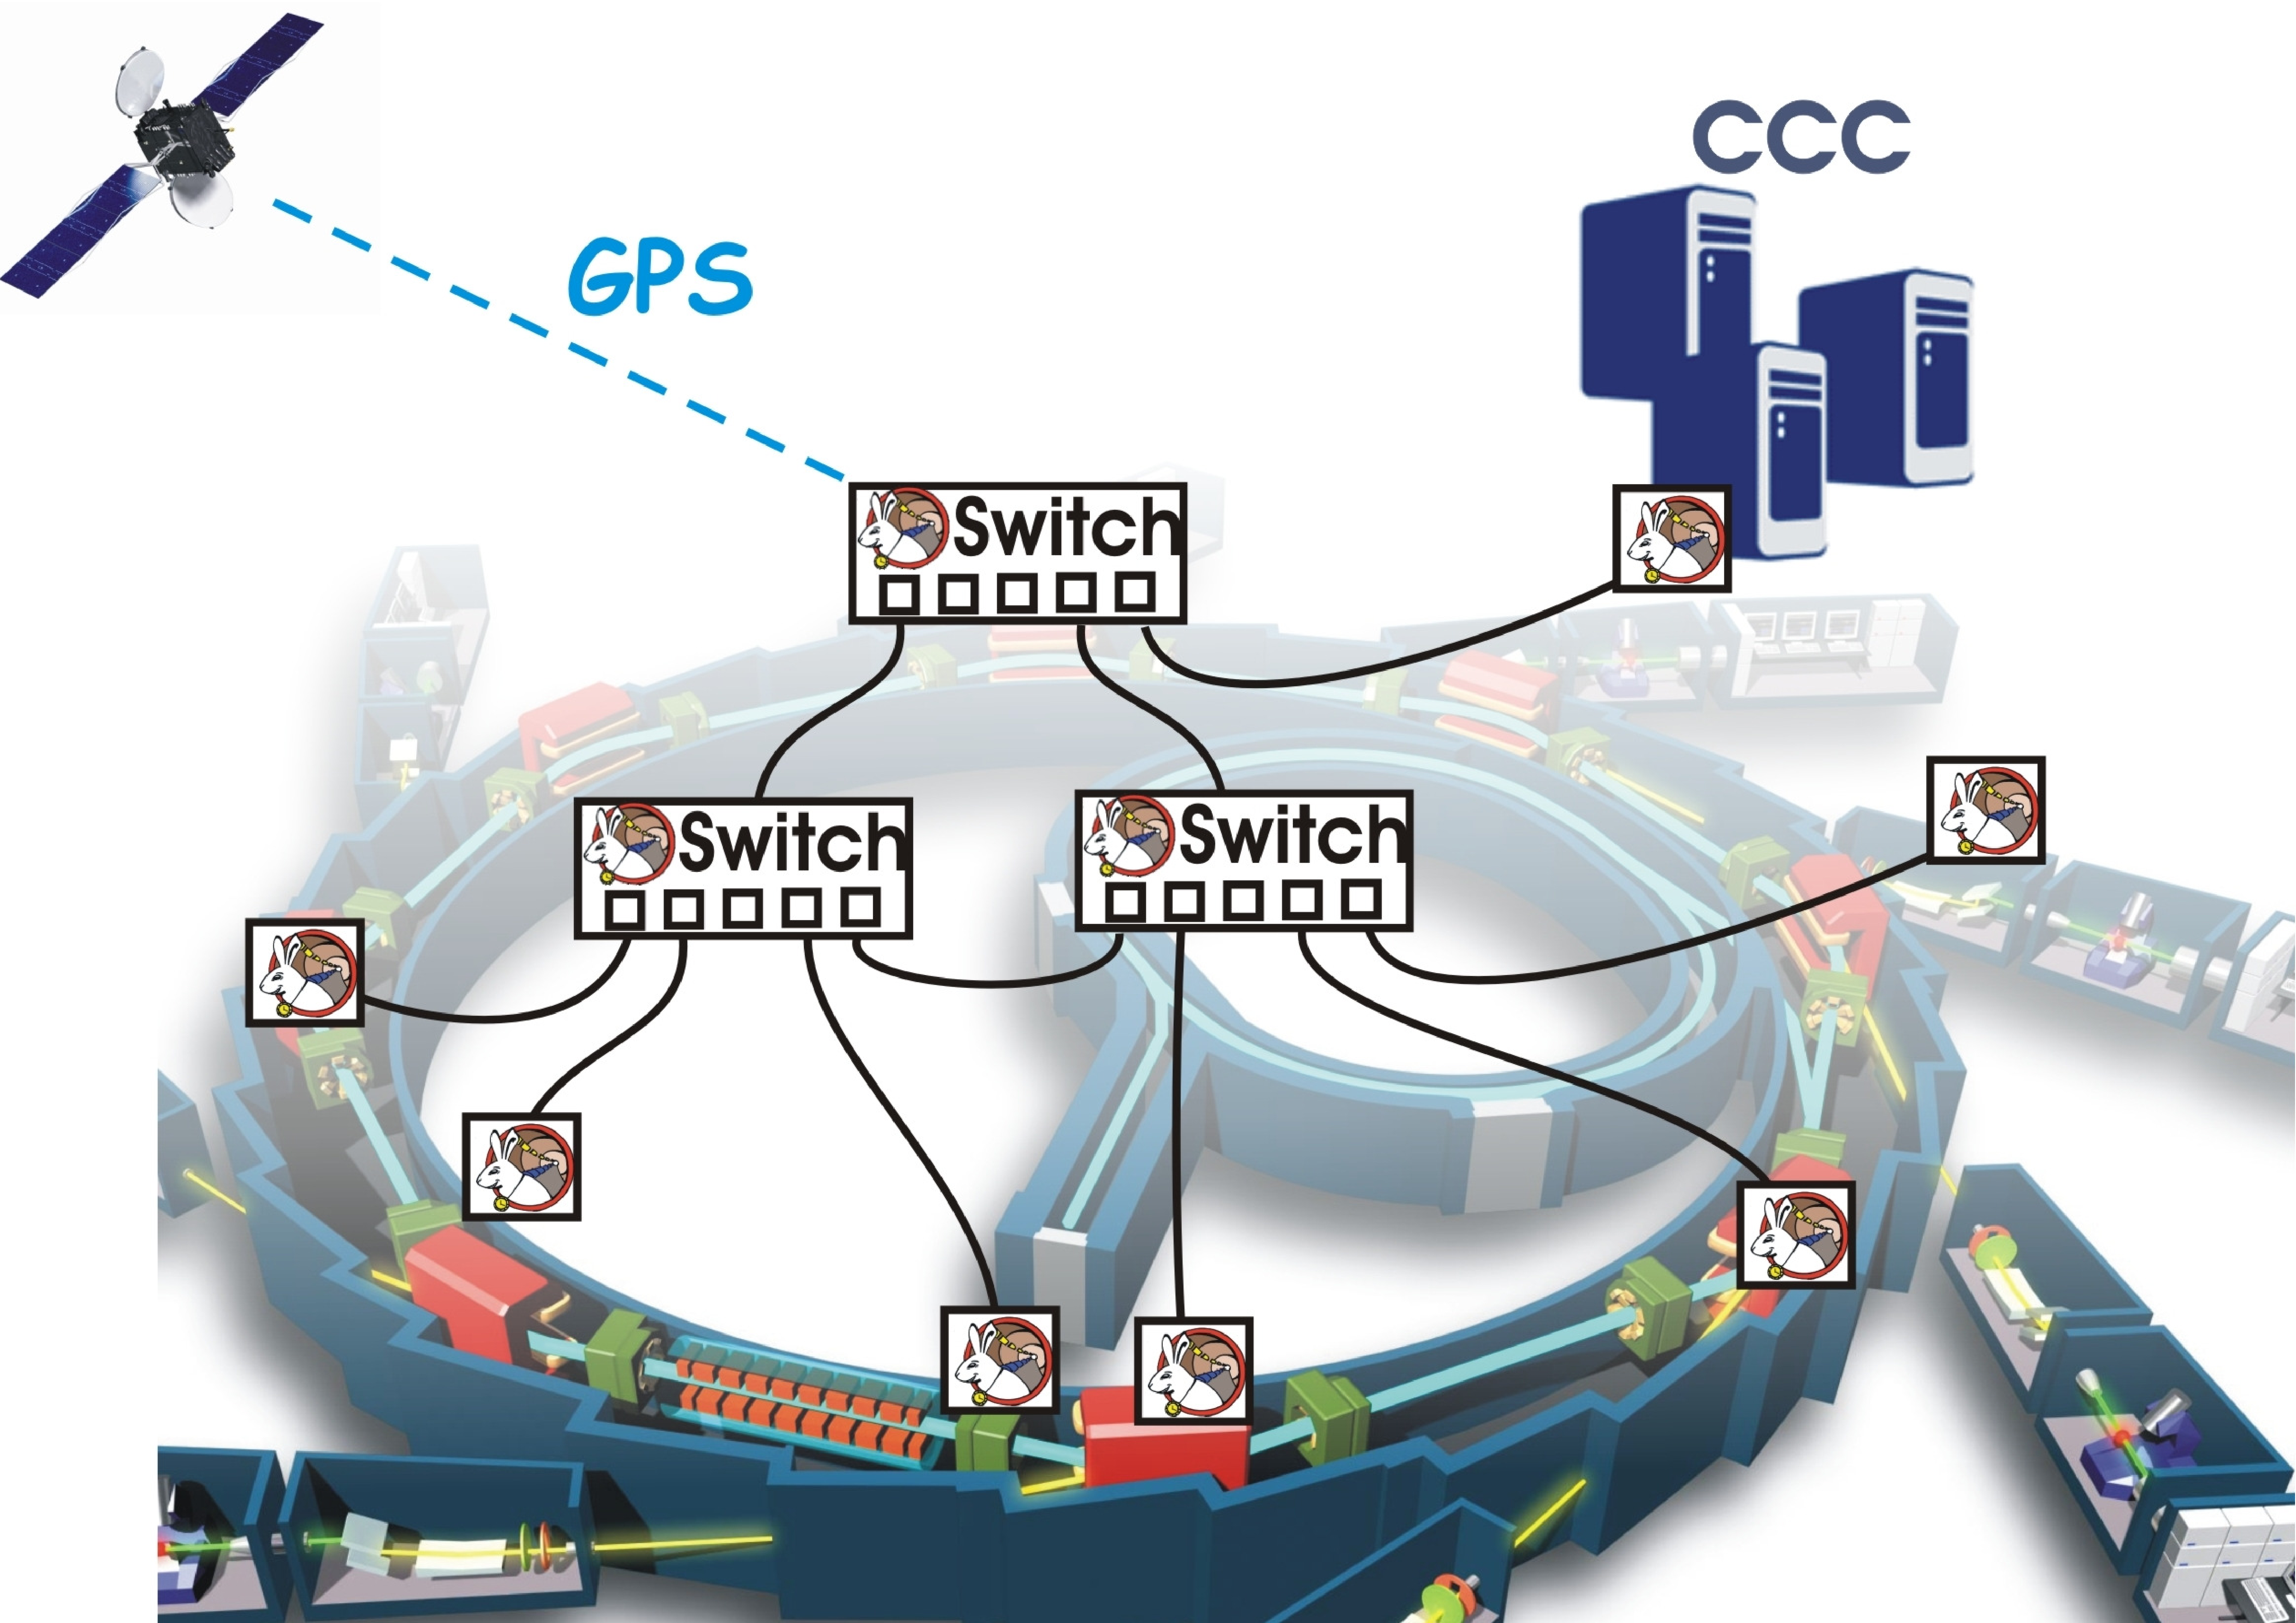
\includegraphics[width=1.0\textwidth]{applications/CERN/WRcontrol.pdf}
    \end{center}

\end{frame}
%%%%%%%%%%%%%%%%%%%%%%%%%%%%%%%%%%%%%%%%%%%%%%%%%%%%%%%%%%%%%%%%%%%%%%%%%%%%%%%%%%%%%%%%%%%%%%%%%%%%
%\subsection{What is White Rabbit?}
%%%%%%%%%%%%%%%%%%%%%%%%%%%%%%%%%%%%%%%%%%%%%%%%%%%%%%%%%%%%%%%%%%%%%%%%%%%%%%%%%%%%%%%%%%%%%%%%%%%%
\begin{frame}{Sieć White Rabbit}

\begin{columns}[c]
  \column{.47\textwidth}

  \begin{itemize}
    \item \color{blue!90}{Sub-nanosekundowa synchronizacja}
    \vspace{0.2cm}
    \item \color{red}{Deterministyczna i niezawodna transmisja informacji kontrolnych (Control Message)}
  \end{itemize}

  \column{.6\textwidth}
    \begin{center}
    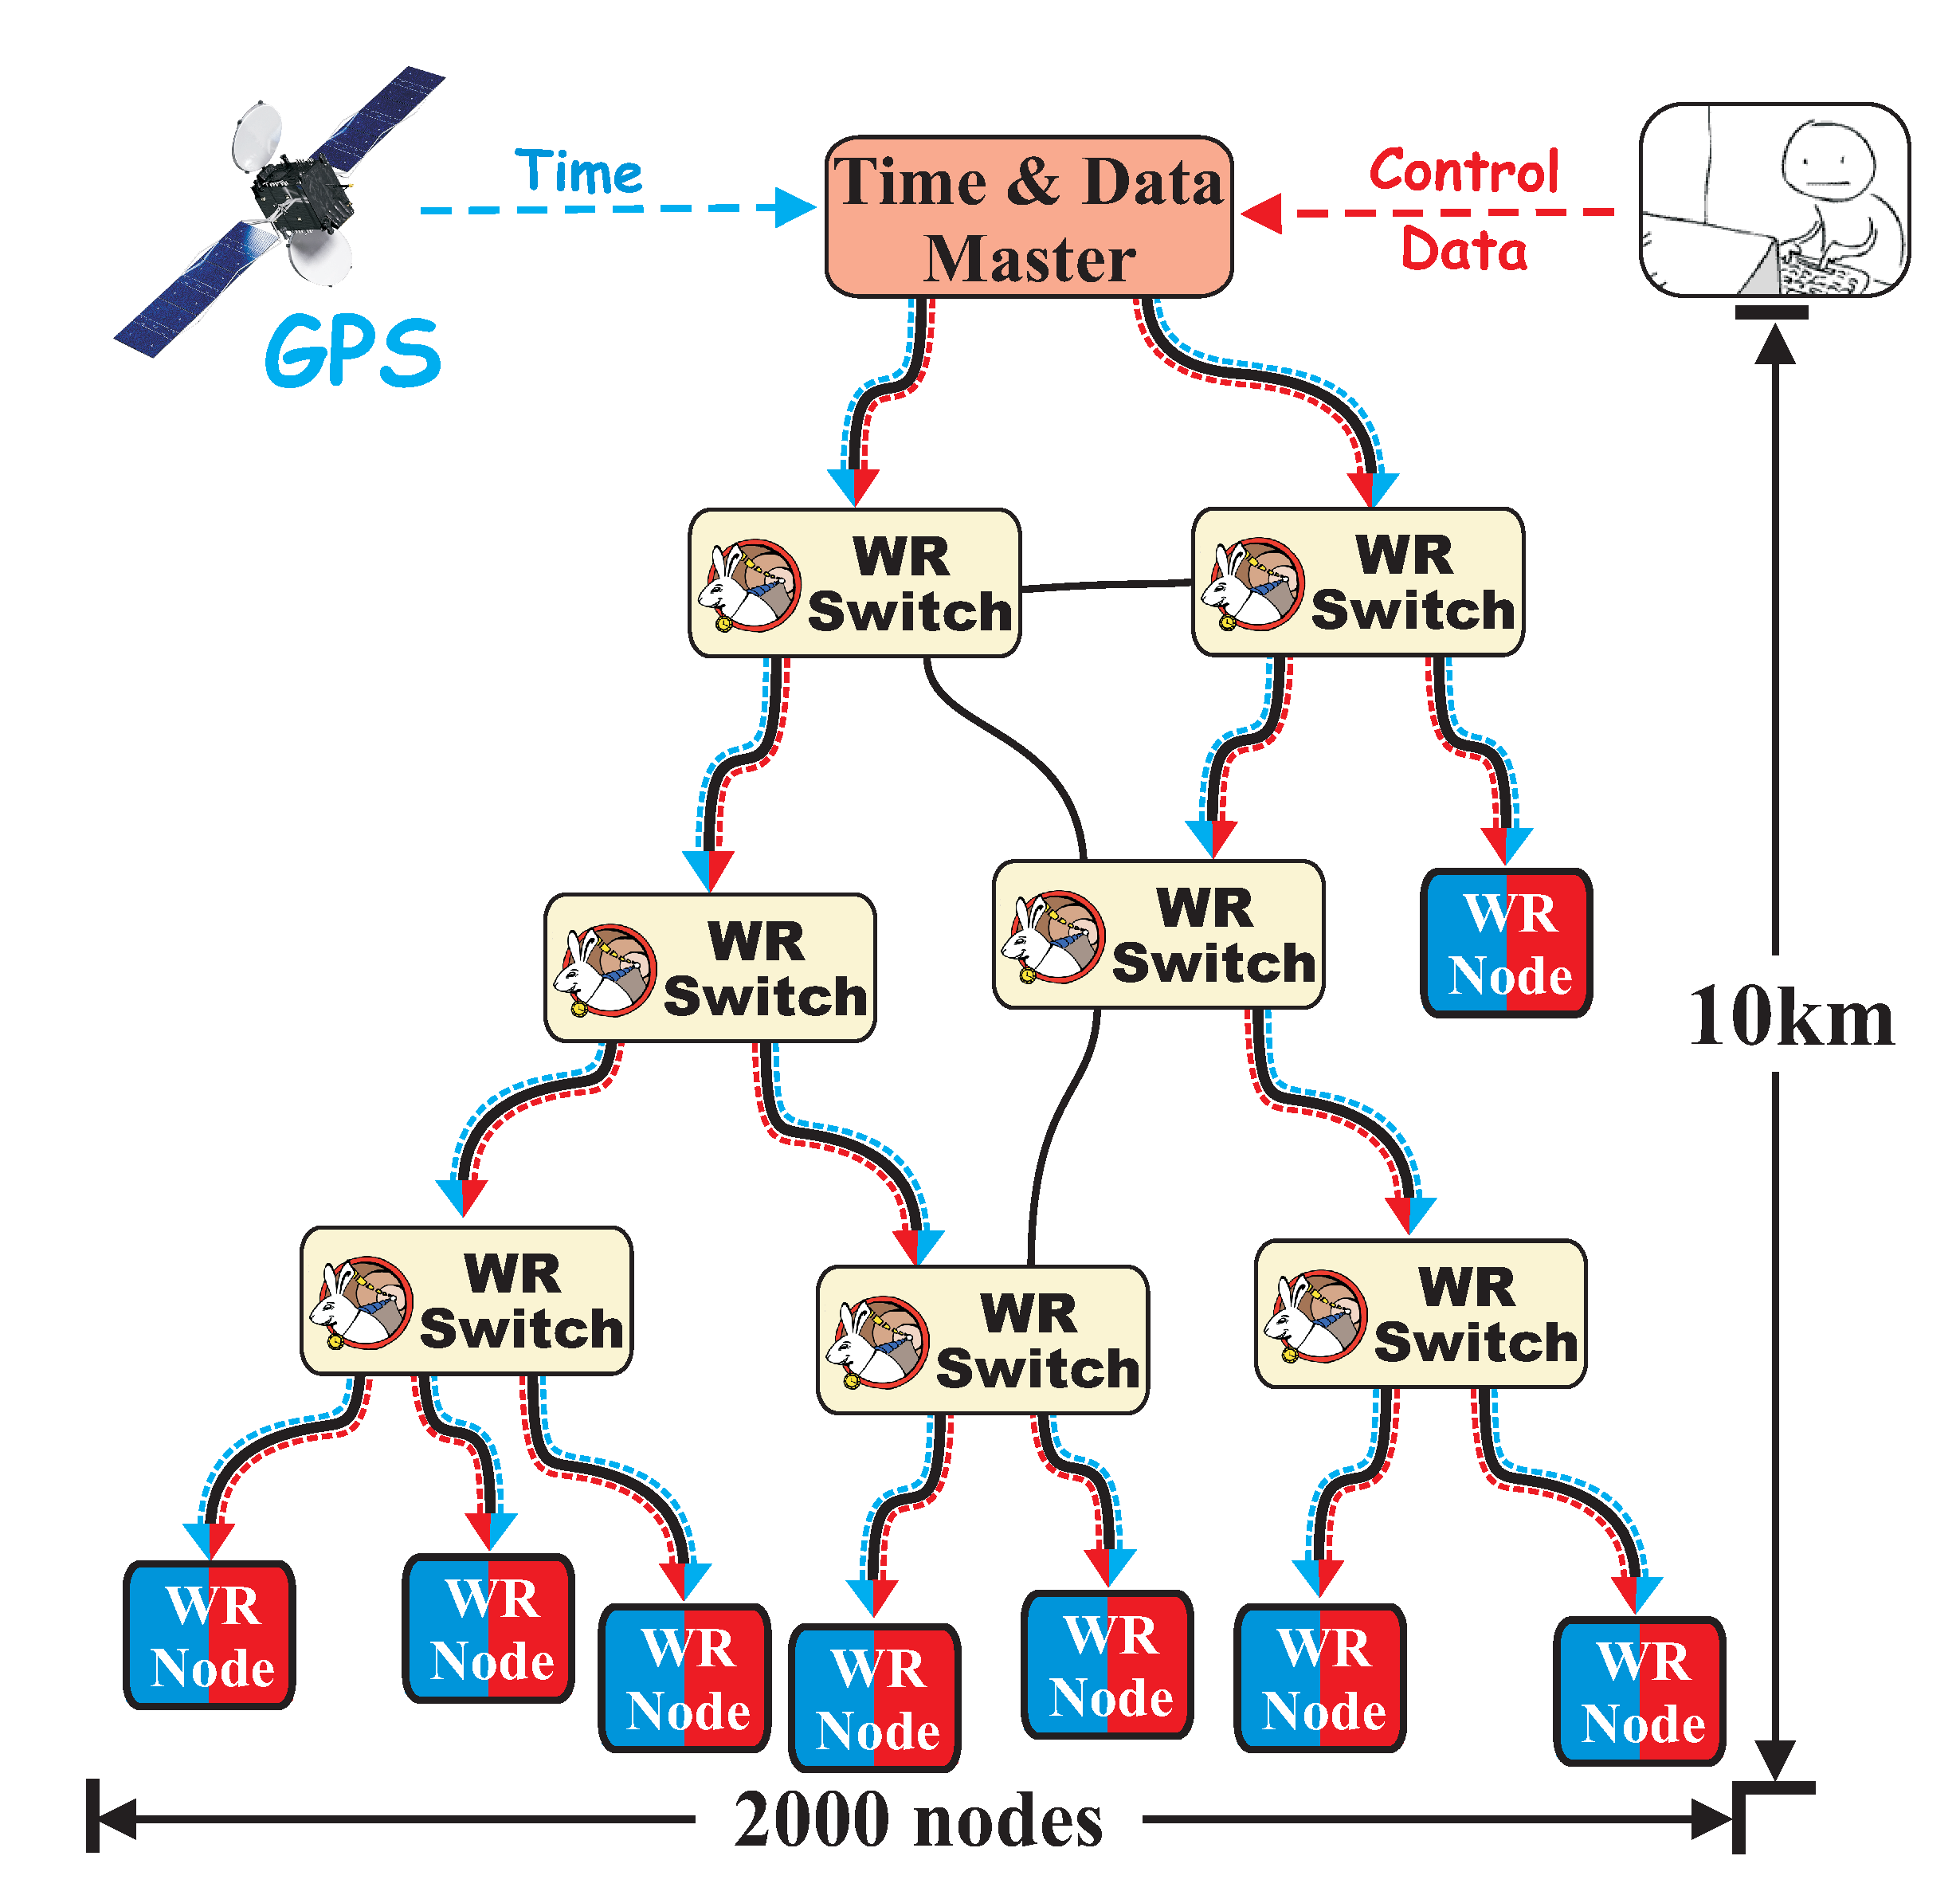
\includegraphics[height=1.0\textwidth]{network/wr_network-new.pdf}
    \end{center}
\end{columns}

\end{frame}
%%%%%%%%%%%%%%%%%%%%%%%%%%%%%%%%%%%%%%%%%%%%%%%%%%%%%%%%%%%%%%%%%%%%%%%%%%%%%%%%%%%%%%%%%%%%%%%%%%%%
\section{Dystrybucja czasu w sieci WR}
\subsection{}
%%%%%%%%%%%%%%%%%%%%%%%%%%%%%%%%%%%%%%%%%%%%%%%%%%%%%%%%%%%%%%%%%%%%%%%%%%%%%%%%%%%%%%%%%%%%%%%%%%%%
\begin{frame}{Dystrybucja czasu w sieci White Rabbit}

 \begin{center}
    \color{blue!90}{Sub-nanosekundowa synchronizacja}
  \end{center}

\end{frame}
%%%%%%%%%%%%%%%%%%%%%%%%%%%%%%%%%%%%%%%%%%%%%%%%%%%%%%%%%%%%%%%%%%%%%%%%%%%%%%%%%%%%%%%%%%%%%%%%%%%%
% \subsection{}
%%%%%%%%%%%%%%%%%%%%%%%%%%%%%%%%%%%%%%%%%%%%%%%%%%%%%%%%%%%%%%%%%%%%%%%%%%%%%%%%%%%%%%%%%%%%%%%%%%%%
\begin{frame}{Podstawowe pojęcia}

  \begin{itemize}
    \item Synchronizacja z {\bf sub-nanosekundową} dokładnością po światłowodzie,
    \item Połączenie
	\begin{itemize}
%	  \item Precision Time Protocol ({\bf PTP}) - synchronizacja,
%	  \item Synchronous Ethernet ({\bf SyncE}) syntonizacja,
%	  \item Digital Dual-Mixer Time Difference ({\bf DDMTD}) - pomiar fazy,
	  \item Precision Time Protocol (\color{blue}{PTP}\color{black}{) - synchronizacja,}
	  \item Synchronous Ethernet (\color{blue}{SyncE}\color{black}{) syntonizacja,}
	  \item Digital Dual-Mixer Time Difference (\color{blue}{DDMTD}\color{black}{) - pomiar fazy,}

	\end{itemize}
%    \item Reliability-oriented.
    \item Połączenie WR (WR Link):
  \end{itemize}

\begin{columns}[c]
  \column{.6\textwidth}

  \begin{center}
  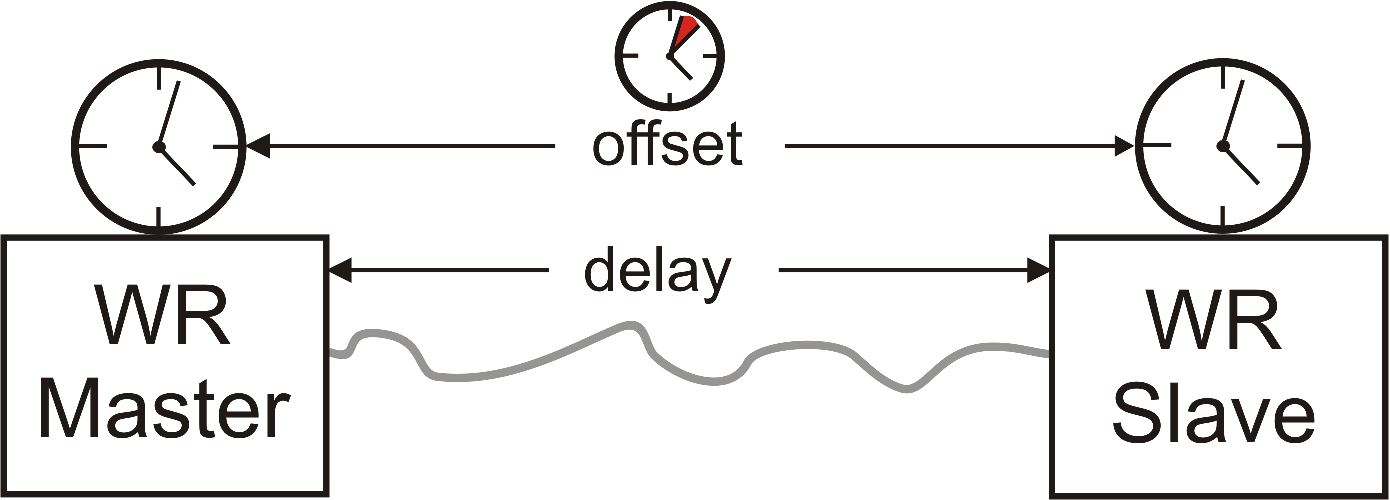
\includegraphics[height=2.5cm]{protocol/wrLink.pdf}
  \end{center}

  \vspace{2cm}

  \column{.4\textwidth}

  \begin{center}
  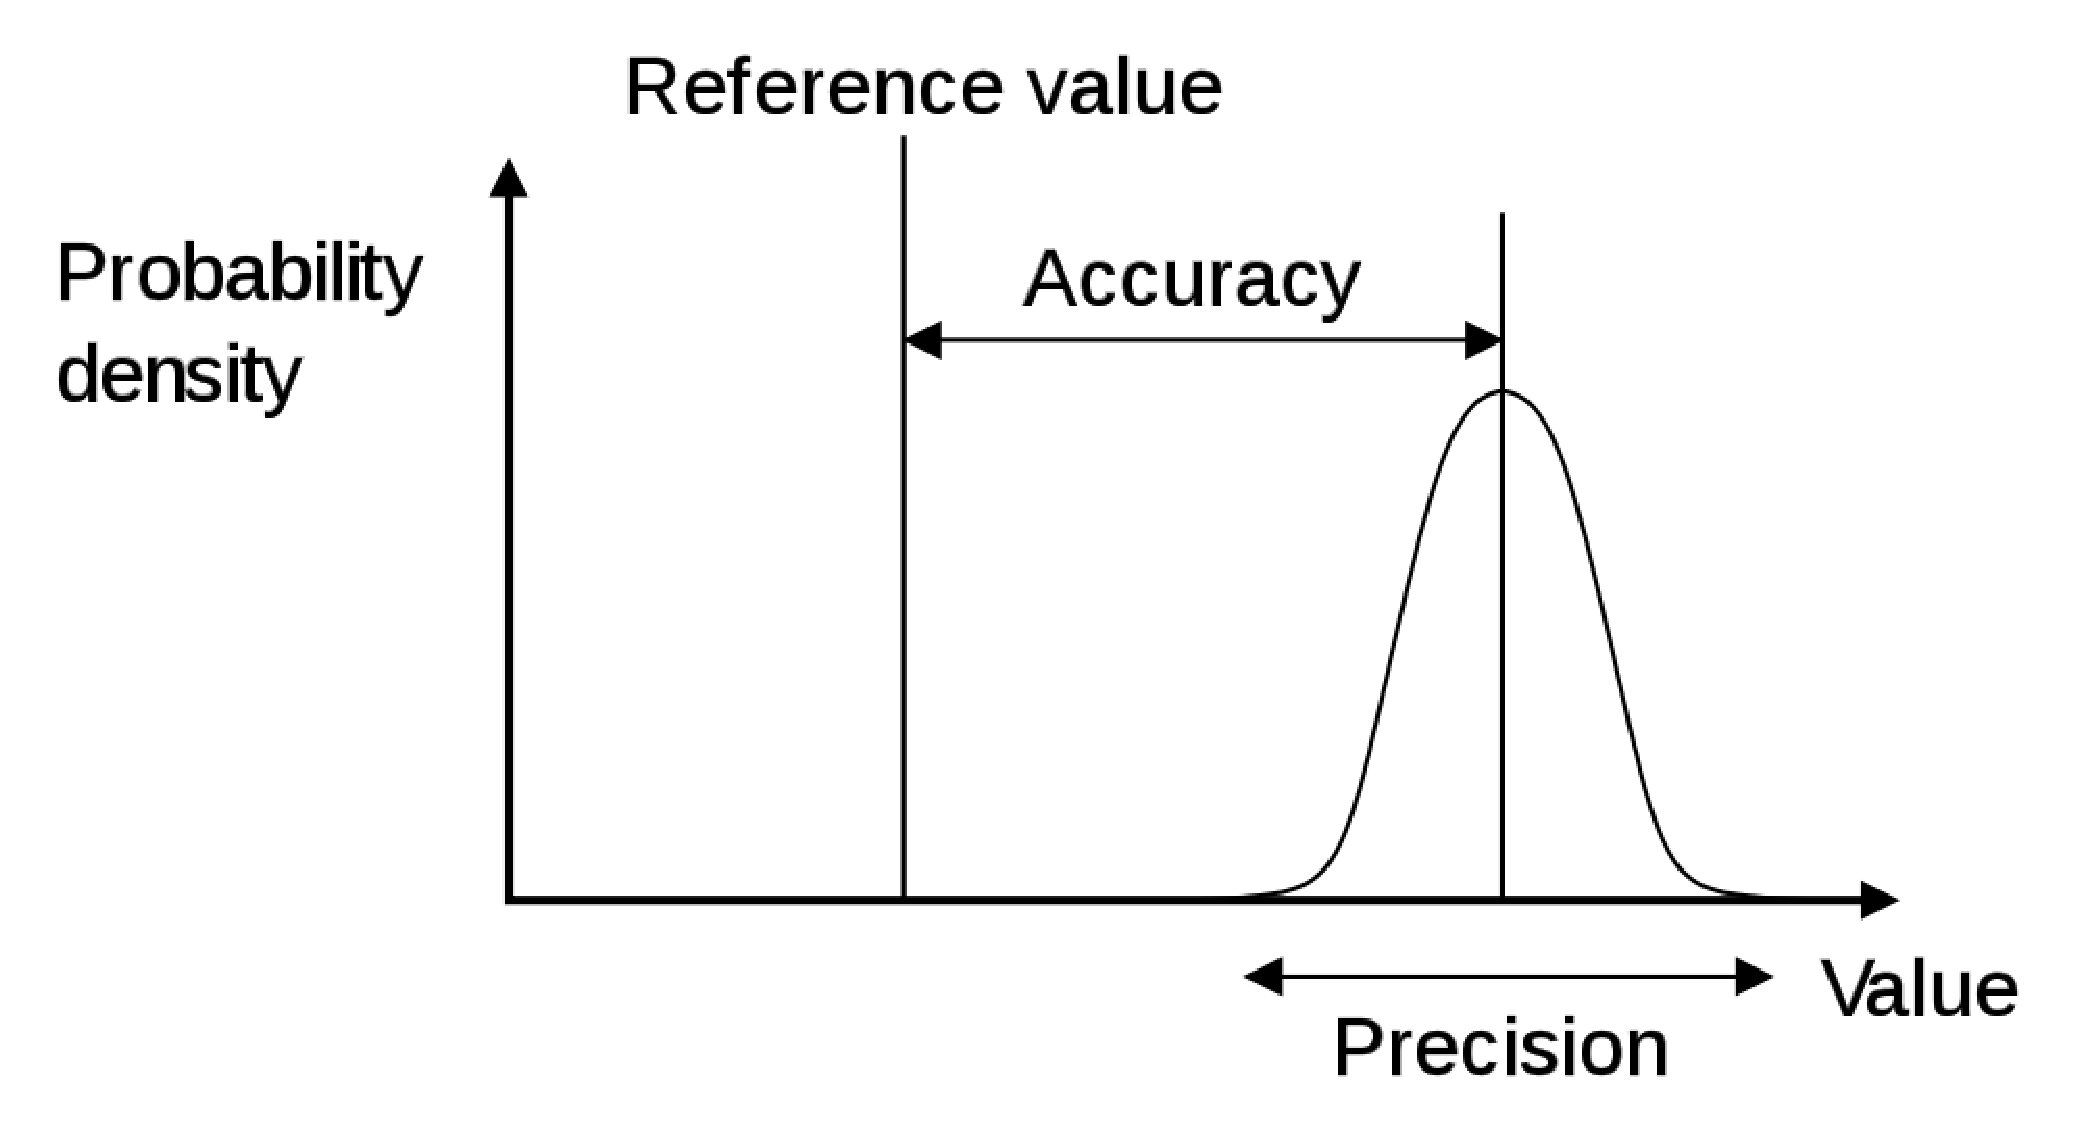
\includegraphics[height=2.6cm]{misc/Accuracy_and_precision.pdf}
  \end{center}

  \vspace{1cm}

\end{columns}


\end{frame}

%%%%%%%%%%%%%%%%%%%%%%%%%%%%%%%%%%%%%%%%%%%%%%%%%%%%%%%%%%%%%%%%%%%%%%%%%%%%%%%%%%%%%%%%%%%%%%%%%%%%
% \subsection{}
%%%%%%%%%%%%%%%%%%%%%%%%%%%%%%%%%%%%%%%%%%%%%%%%%%%%%%%%%%%%%%%%%%%%%%%%%%%%%%%%%%%%%%%%%%%%%%%%%%%%
%\beamertemplatesolidbackgroundcolor{black}
\begin{frame}{Sieć White Rabbit}
%\beamertemplatesolidbackgroundcolor{black}
\center Sieć White Rabbit
  \begin{center}
  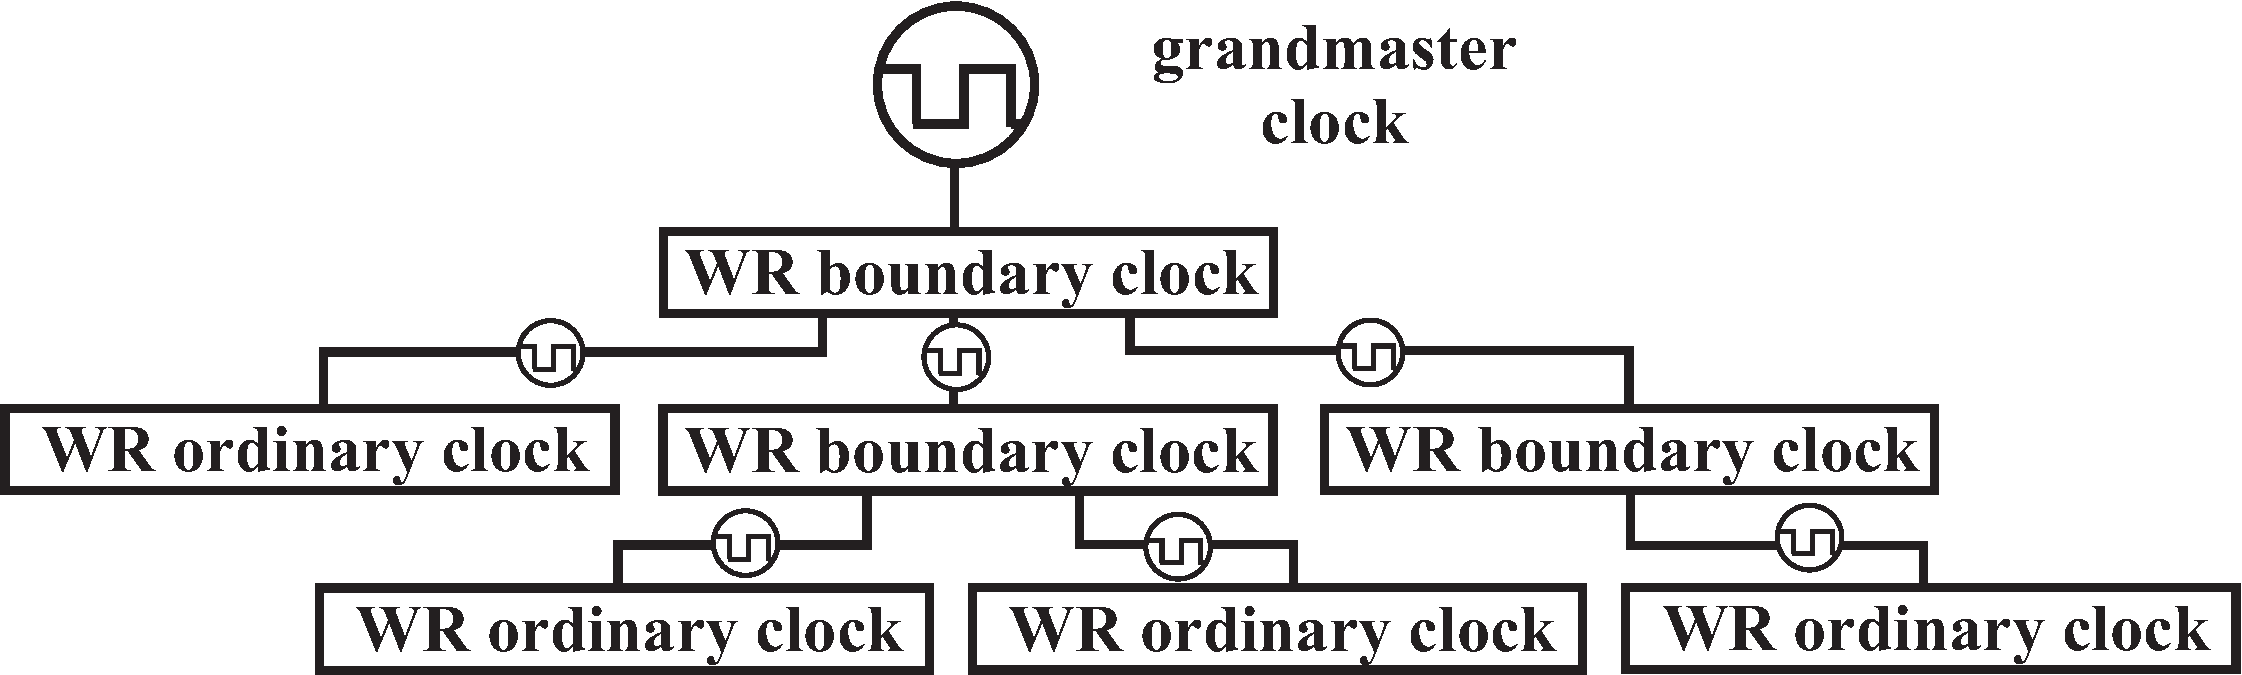
\includegraphics[width=11.5cm]{network/wrTopology.pdf}
%\includegraphics[height=6cm]{fig/front.eps}
  \end{center}
\end{frame}
%%%%%%%%%%%%%%%%%%%%%%%%%%%%%%%%%%%%%%%%%%%%%%%%%%%%%%%%%%%%%%%%%%%%%%%%%%%%%%%%%%%%%%%%%%%%%%%%%%%%
% \section{PTP}
% \subsection{}
\begin{frame}{Precision Time Protocol (PTP)}
%%%%%%%%%%%%%%%%%%%%%%%%%%%%%%%%%%%%%%%%%%%%%%%%%%%%%%%%%%%%%%%%%%%%%%%%%%%%%%%%%%%%%%%%%%%%%%%%%%%%
\begin{columns}[c]
\column{2.8in}

  \begin{itemize}
    \item standard IEEE1588-2008
    \item protokół oparty na wymianie pakietów
    \item synchronizacja urządzeń w systemach rozproszonych
  \end{itemize}

\column{1.5in}
    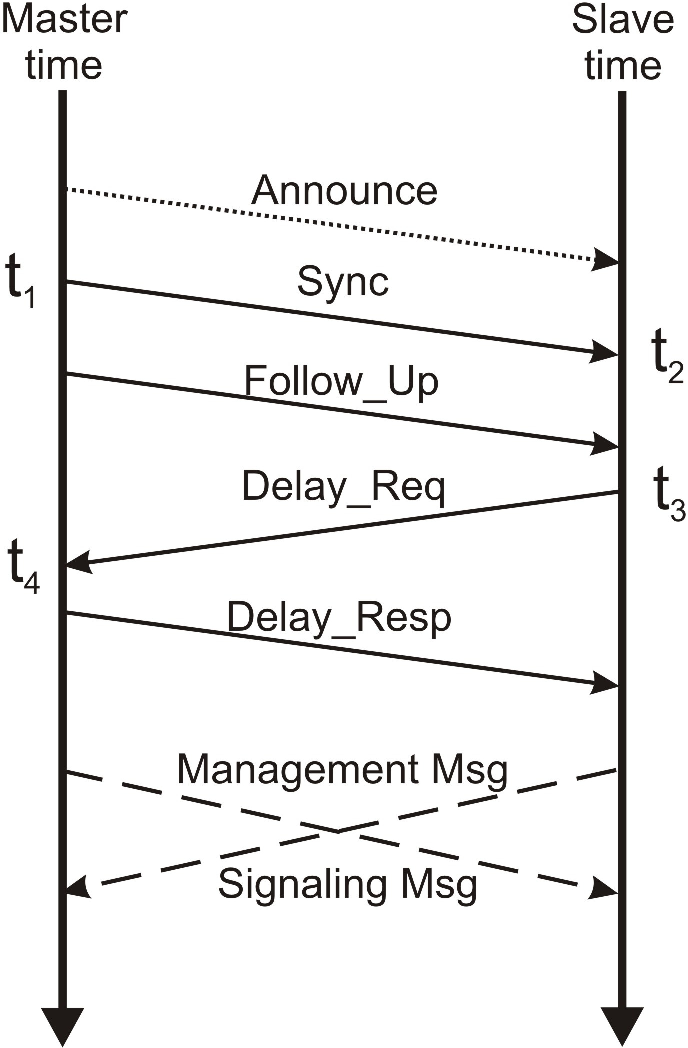
\includegraphics[height=5.5cm]{protocol/ptpMSGs.pdf} \\
    \small 
    one-way mean delay: \\
    $\mu = \frac{(t_{4}-t_{1}) - (t_{3}-t_{2})}{2}$ \\
    \small 
    $offset = t_{2} - (t_{1} + \mu)$
    
\end{columns}


\end{frame}
%%%%%%%%%%%%%%%%%%%%%%%%%%%%%%%%%%%%%%%%%%%%%%%%%%%%%%%%%%%%%%%%%%%%%%%%%%%%%%%%%%%%%%%%%%%%%%%%%%%%
%\section{Why not standard PTP?}
%\subsection{}
% %%%%%%%%%%%%%%%%%%%%%%%%%%%%%%%%%%%%%%%%%%%%%%%%%%%%%%%%%%%%%%%%%%%%%%%%%%%%%%%%%%%%%%%%%%%%%%%%%%%%
% \begin{frame}{PTP is OK but ...}
% % 
% %   \begin{itemize}
% %     \item Limited precision and resolution,
% %     \item Unknown physical link asymmetry,
% %     \item PTP-based syntonization vs. traffic load.
% %   \end{itemize}
% 
%   \resizebox{11cm}{!} 
%   {
%     \begin{tabular}{ r c l }
%       PTP-base		 	& $=>$ & traffic load  \\
%       syntonization	        &      &        \\
% 				&      &        \\
%       limited             	& $=>$ & limited accuracy \\
%       precision and resolution  &      &  \\
% 				&      &        \\
%       unknown                   &      &   \\
%       physical link asymmetry   & $=>$ & limited accuracy 	\\
% 				&      & \color{white}{DDTMD phase detection}			\\
% 				&      &        		\\
%       \multicolumn{3}{c}{\color{white}{WR extension to PTP ({\bf WRPTP}}) for } \\
%       \multicolumn{3}{c}{\color{white}{extra data exchange and logic}} \\
%     \end{tabular}
%   }
% 
% \end{frame}
%%%%%%%%%%%%%%%%%%%%%%%%%%%%%%%%%%%%%%%%%%%%%%%%%%%%%%%%%%%%%%%%%%%%%%%%%%%%%%%%%%%%%%%%%%%%%%%%%%%%
% \subsection{}
%%%%%%%%%%%%%%%%%%%%%%%%%%%%%%%%%%%%%%%%%%%%%%%%%%%%%%%%%%%%%%%%%%%%%%%%%%%%%%%%%%%%%%%%%%%%%%%%%%%%
%\begin{frame}{Addressing the issues}
\begin{frame}{PTP jest OK ale ...}

  \resizebox{11cm}{!} 
  {
    \begin{tabular}{ r c l }
  {\bf Ograniczenia PTP...} 	& {\bf i}      & {\bf ... jak sobie z nimi radzimy}  \\
				&     		 &        \\
      syntonizacja	 	& \multirow{2}{*}{$\Rightarrow$}  & \multirow{2}{*}{SyncE }\\
      oparta na PTP	        &      		 &        \\
				&      		 &        			\\
      ograniczona             	&\multirow{2}{*}{$\Rightarrow$}  	 & SyncE \\
      dokładność i rozdzielczość&      		 & pomiar fazy przy pomocy DDTMD\\
				&    		 &        \\
			        &      		 & SyncE  \\
      nieznana asymetria łącza  & $\Rightarrow$  & pomiar fazy przy pomocy DDTMD \\
				&      		 & WR Link Delay Model \\
				&      		 &        \\
      \multicolumn{3}{c}{WR extension to PTP ({\bf WRPTP})  } \\
      \multicolumn{3}{c}{pozwala na wymianę dodatkowych parametrów i wykonanie specyficznych dla WR procedur} \\
    \end{tabular}
  }
\end{frame}
% %%%%%%%%%%%%%%%%%%%%%%%%%%%%%%%%%%%%%%%%%%%%%%%%%%%%%%%%%%%%%%%%%%%%%%%%%%%%%%%%%%%%%%%%%%%%%%%%%%%%
% \section{Technologies}
% \subsection{}
% %%%%%%%%%%%%%%%%%%%%%%%%%%%%%%%%%%%%%%%%%%%%%%%%%%%%%%%%%%%%%%%%%%%%%%%%%%%%%%%%%%%%%%%%%%%%%%%%%%%%
% \begin{frame}{SyncE syntonization}
% 
% {\it [(1)Steal an animation by Eva ?]} \\
% {\it [(2)Remove ?]}
% 
% \end{frame}
%%%%%%%%%%%%%%%%%%%%%%%%%%%%%%%%%%%%%%%%%%%%%%%%%%%%%%%%%%%%%%%%%%%%%%%%%%%%%%%%%%%%%%%%%%%%%%%%%%%%
% \subsection{}
%%%%%%%%%%%%%%%%%%%%%%%%%%%%%%%%%%%%%%%%%%%%%%%%%%%%%%%%%%%%%%%%%%%%%%%%%%%%%%%%%%%%%%%%%%%%%%%%%%%%
% \begin{frame}{DDMTD phase detection}
% 
% {\it[remove ?]}
% 
%   \begin{center}
%   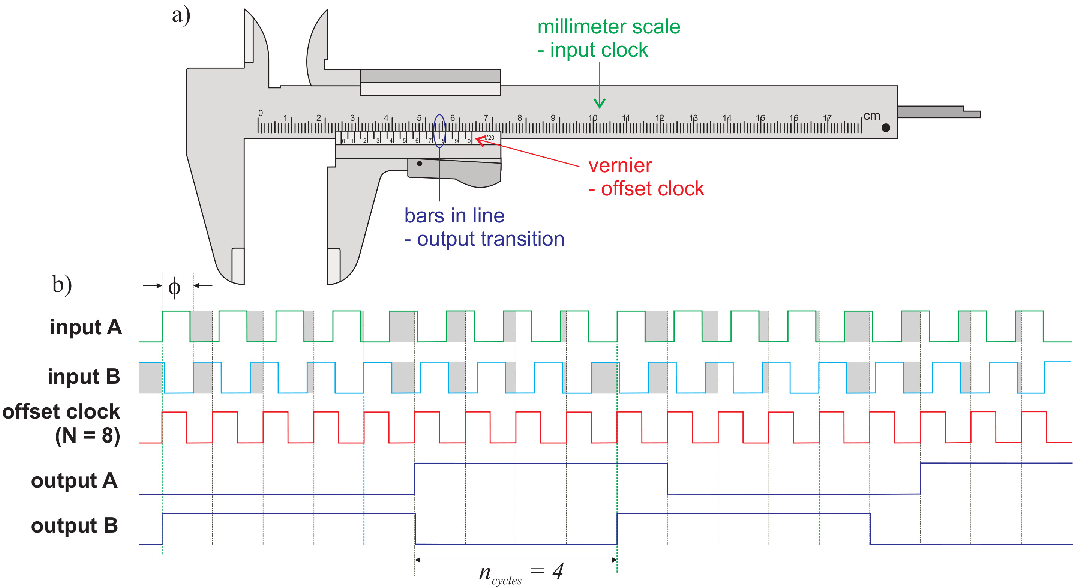
\includegraphics[width=11cm]{fig/dmtd_vernier.eps}
%   \end{center}
% 
% \end{frame}
%%%%%%%%%%%%%%%%%%%%%%%%%%%%%%%%%%%%%%%%%%%%%%%%%%%%%%%%%%%%%%%%%%%%%%%%%%%%%%%%%%%%%%%%%%%%%%%%%%%%
%\section{Link Delay Model}
%\subsection{}
%%%%%%%%%%%%%%%%%%%%%%%%%%%%%%%%%%%%%%%%%%%%%%%%%%%%%%%%%%%%%%%%%%%%%%%%%%%%%%%%%%%%%%%%%%%%%%%%%%%%
\begin{frame}{Link Delay Model}

  \begin{align}
    \nonumber delay_{ms} &= \Delta_{tx_m} + \delta_{ms} + \Delta_{rx_s} \\
    \nonumber delay_{sm} &= \Delta_{tx_s} + \delta_{sm} + \Delta_{rx_m}
  \end{align}

   \vspace{0.2cm}

  \begin{center}
  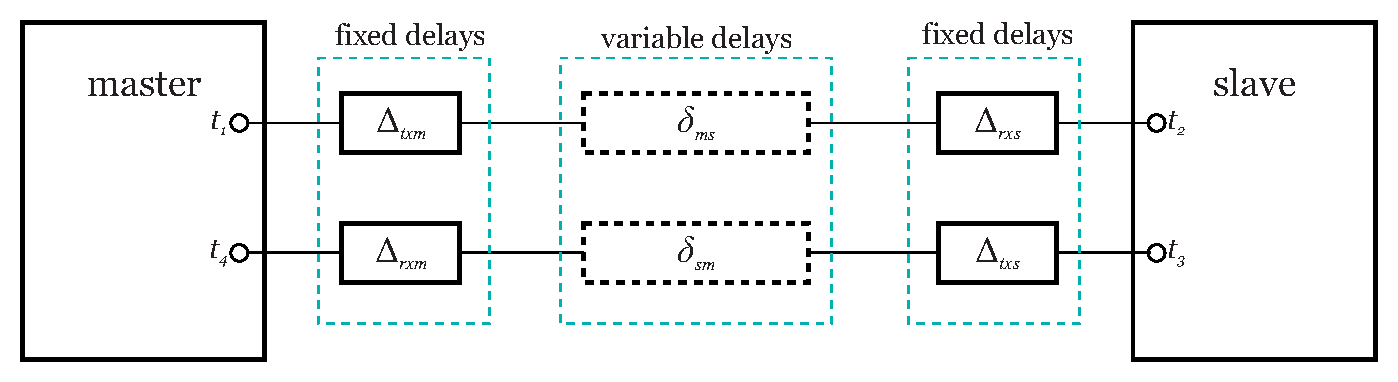
\includegraphics[height=2.5cm]{protocol/delaymodel.pdf}
  \end{center}

\begin{columns}[c]
  \column{2.8in}

    \begin{center}
      \textbf{Relative Delay Coefficient ($\alpha$)} \\
      dla jedno-modowego światłowodu 1000base-X
    \end{center}

  \column{1.5in}
    \begin{center}
      \begin{equation}
      \nonumber \delta_{ms} = (1 + \alpha) \, \delta_{sm}
      \end{equation}
    \end{center}
    \vspace{0.5cm}
\end{columns}
  

\end{frame}
%%%%%%%%%%%%%%%%%%%%%%%%%%%%%%%%%%%%%%%%%%%%%%%%%%%%%%%%%%%%%%%%%%%%%%%%%%%%%%%%%%%%%%%%%%%%%%%%%%%%
% \subsection{}
%%%%%%%%%%%%%%%%%%%%%%%%%%%%%%%%%%%%%%%%%%%%%%%%%%%%%%%%%%%%%%%%%%%%%%%%%%%%%%%%%%%%%%%%%%%%%%%%%%%%
\begin{frame}{Link Delay Model dla światłowodu}

  \begin{center}
  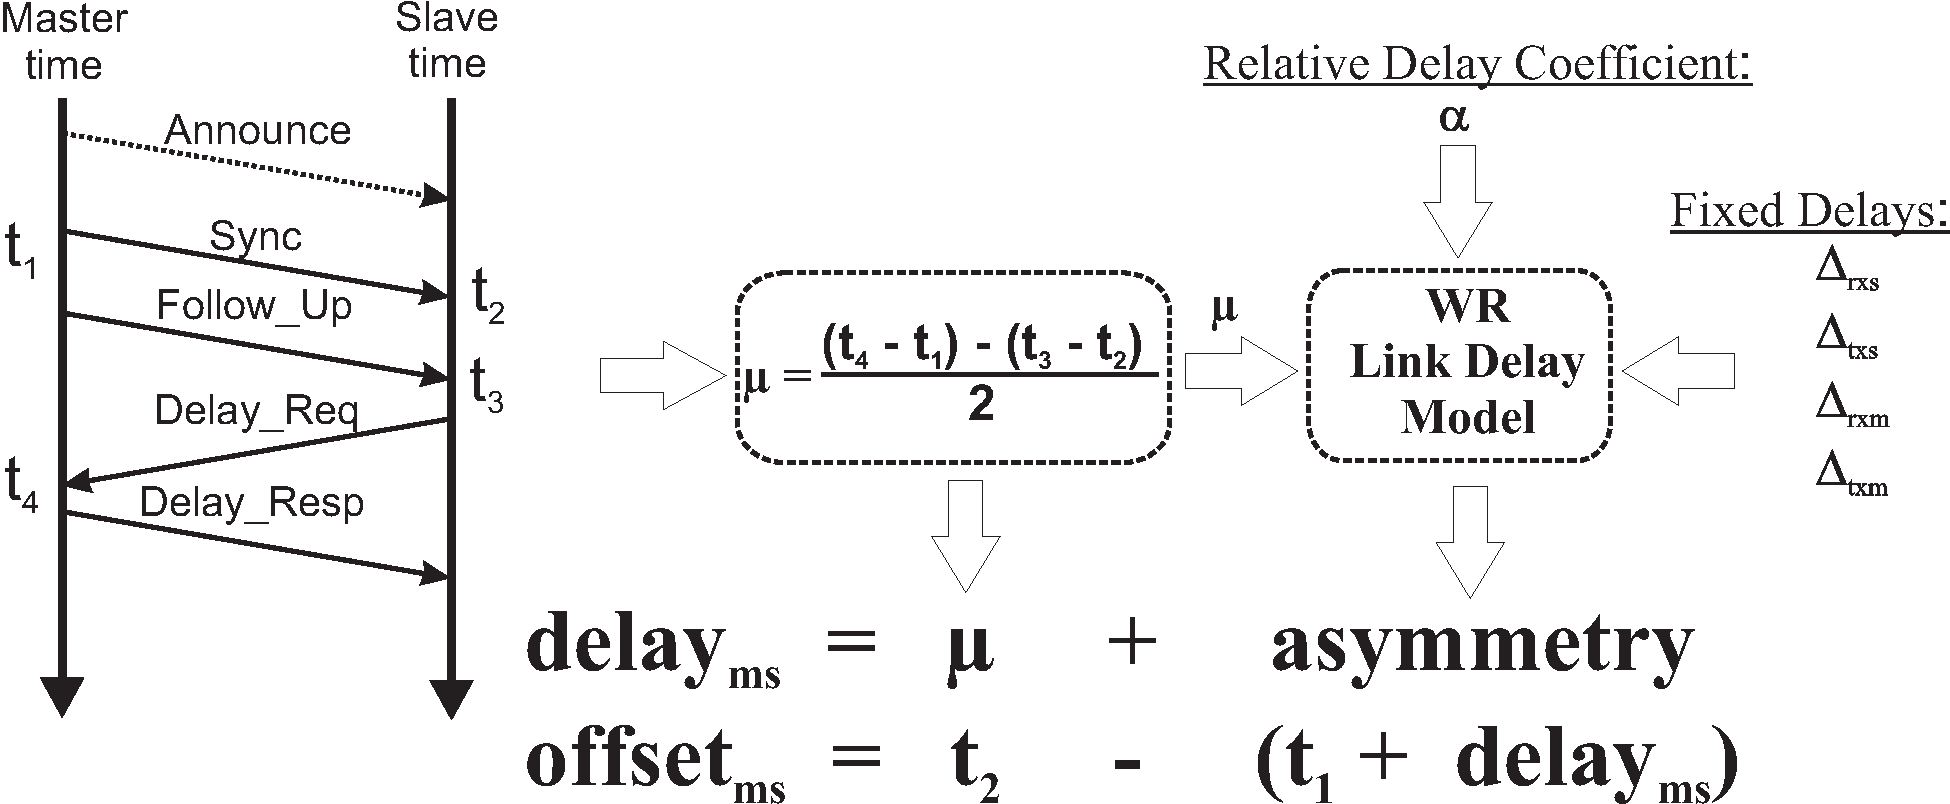
\includegraphics[height=4cm]{protocol/wrLinkModel.pdf}
  \end{center}

  \begin{columns}[c]
  \column{1.5in}

    \begin{center}
      \textbf{Solution for Ethernet over a Single-mode Optical Fiber}
    \end{center}    

  \column{2.7in}

    \begin{equation}
      \nonumber asymmetry = \Delta_{tx_m} + \Delta_{rx_s} - \frac{\Delta - \alpha \mu + \alpha \Delta}{2 + \alpha}
    \end{equation}

  \end{columns}

\end{frame}
% %%%%%%%%%%%%%%%%%%%%%%%%%%%%%%%%%%%%%%%%%%%%%%%%%%%%%%%%%%%%%%%%%%%%%%%%%%%%%%%%%%%%%%%%%%%%%%%%%%%%
% \section{}
% \subsection{}
% %%%%%%%%%%%%%%%%%%%%%%%%%%%%%%%%%%%%%%%%%%%%%%%%%%%%%%%%%%%%%%%%%%%%%%%%%%%%%%%%%%%%%%%%%%%%%%%%%%%%
% \begin{frame}{Overview of White Rabbit Distribution}
% 
% fill in
% 
% \end{frame}
%%%%%%%%%%%%%%%%%%%%%%%%%%%%%%%%%%%%%%%%%%%%%%%%%%%%%%%%%%%%%%%%%%%%%%%%%%%%%%%%%%%%%%%%%%%%%%%%%%%%
%\section{H/W for WR}
%\subsection{}
%%%%%%%%%%%%%%%%%%%%%%%%%%%%%%%%%%%%%%%%%%%%%%%%%%%%%%%%%%%%%%%%%%%%%%%%%%%%%%%%%%%%%%%%%%%%%%%%%%%%
% \begin{frame}{HW4WR}
% 
%   \begin{itemize}
%     \item Fine Delay Measurement,
%     \item Clock Recovery System,
%     \item Fixed Delays Measurement.
%   \end{itemize}
% 
% 
% \end{frame}
%%%%%%%%%%%%%%%%%%%%%%%%%%%%%%%%%%%%%%%%%%%%%%%%%%%%%%%%%%%%%%%%%%%%%%%%%%%%%%%%%%%%%%%%%%%%%%%%%%%%
% \subsection{}
%%%%%%%%%%%%%%%%%%%%%%%%%%%%%%%%%%%%%%%%%%%%%%%%%%%%%%%%%%%%%%%%%%%%%%%%%%%%%%%%%%%%%%%%%%%%%%%%%%%%
\setbeamertemplate{background}{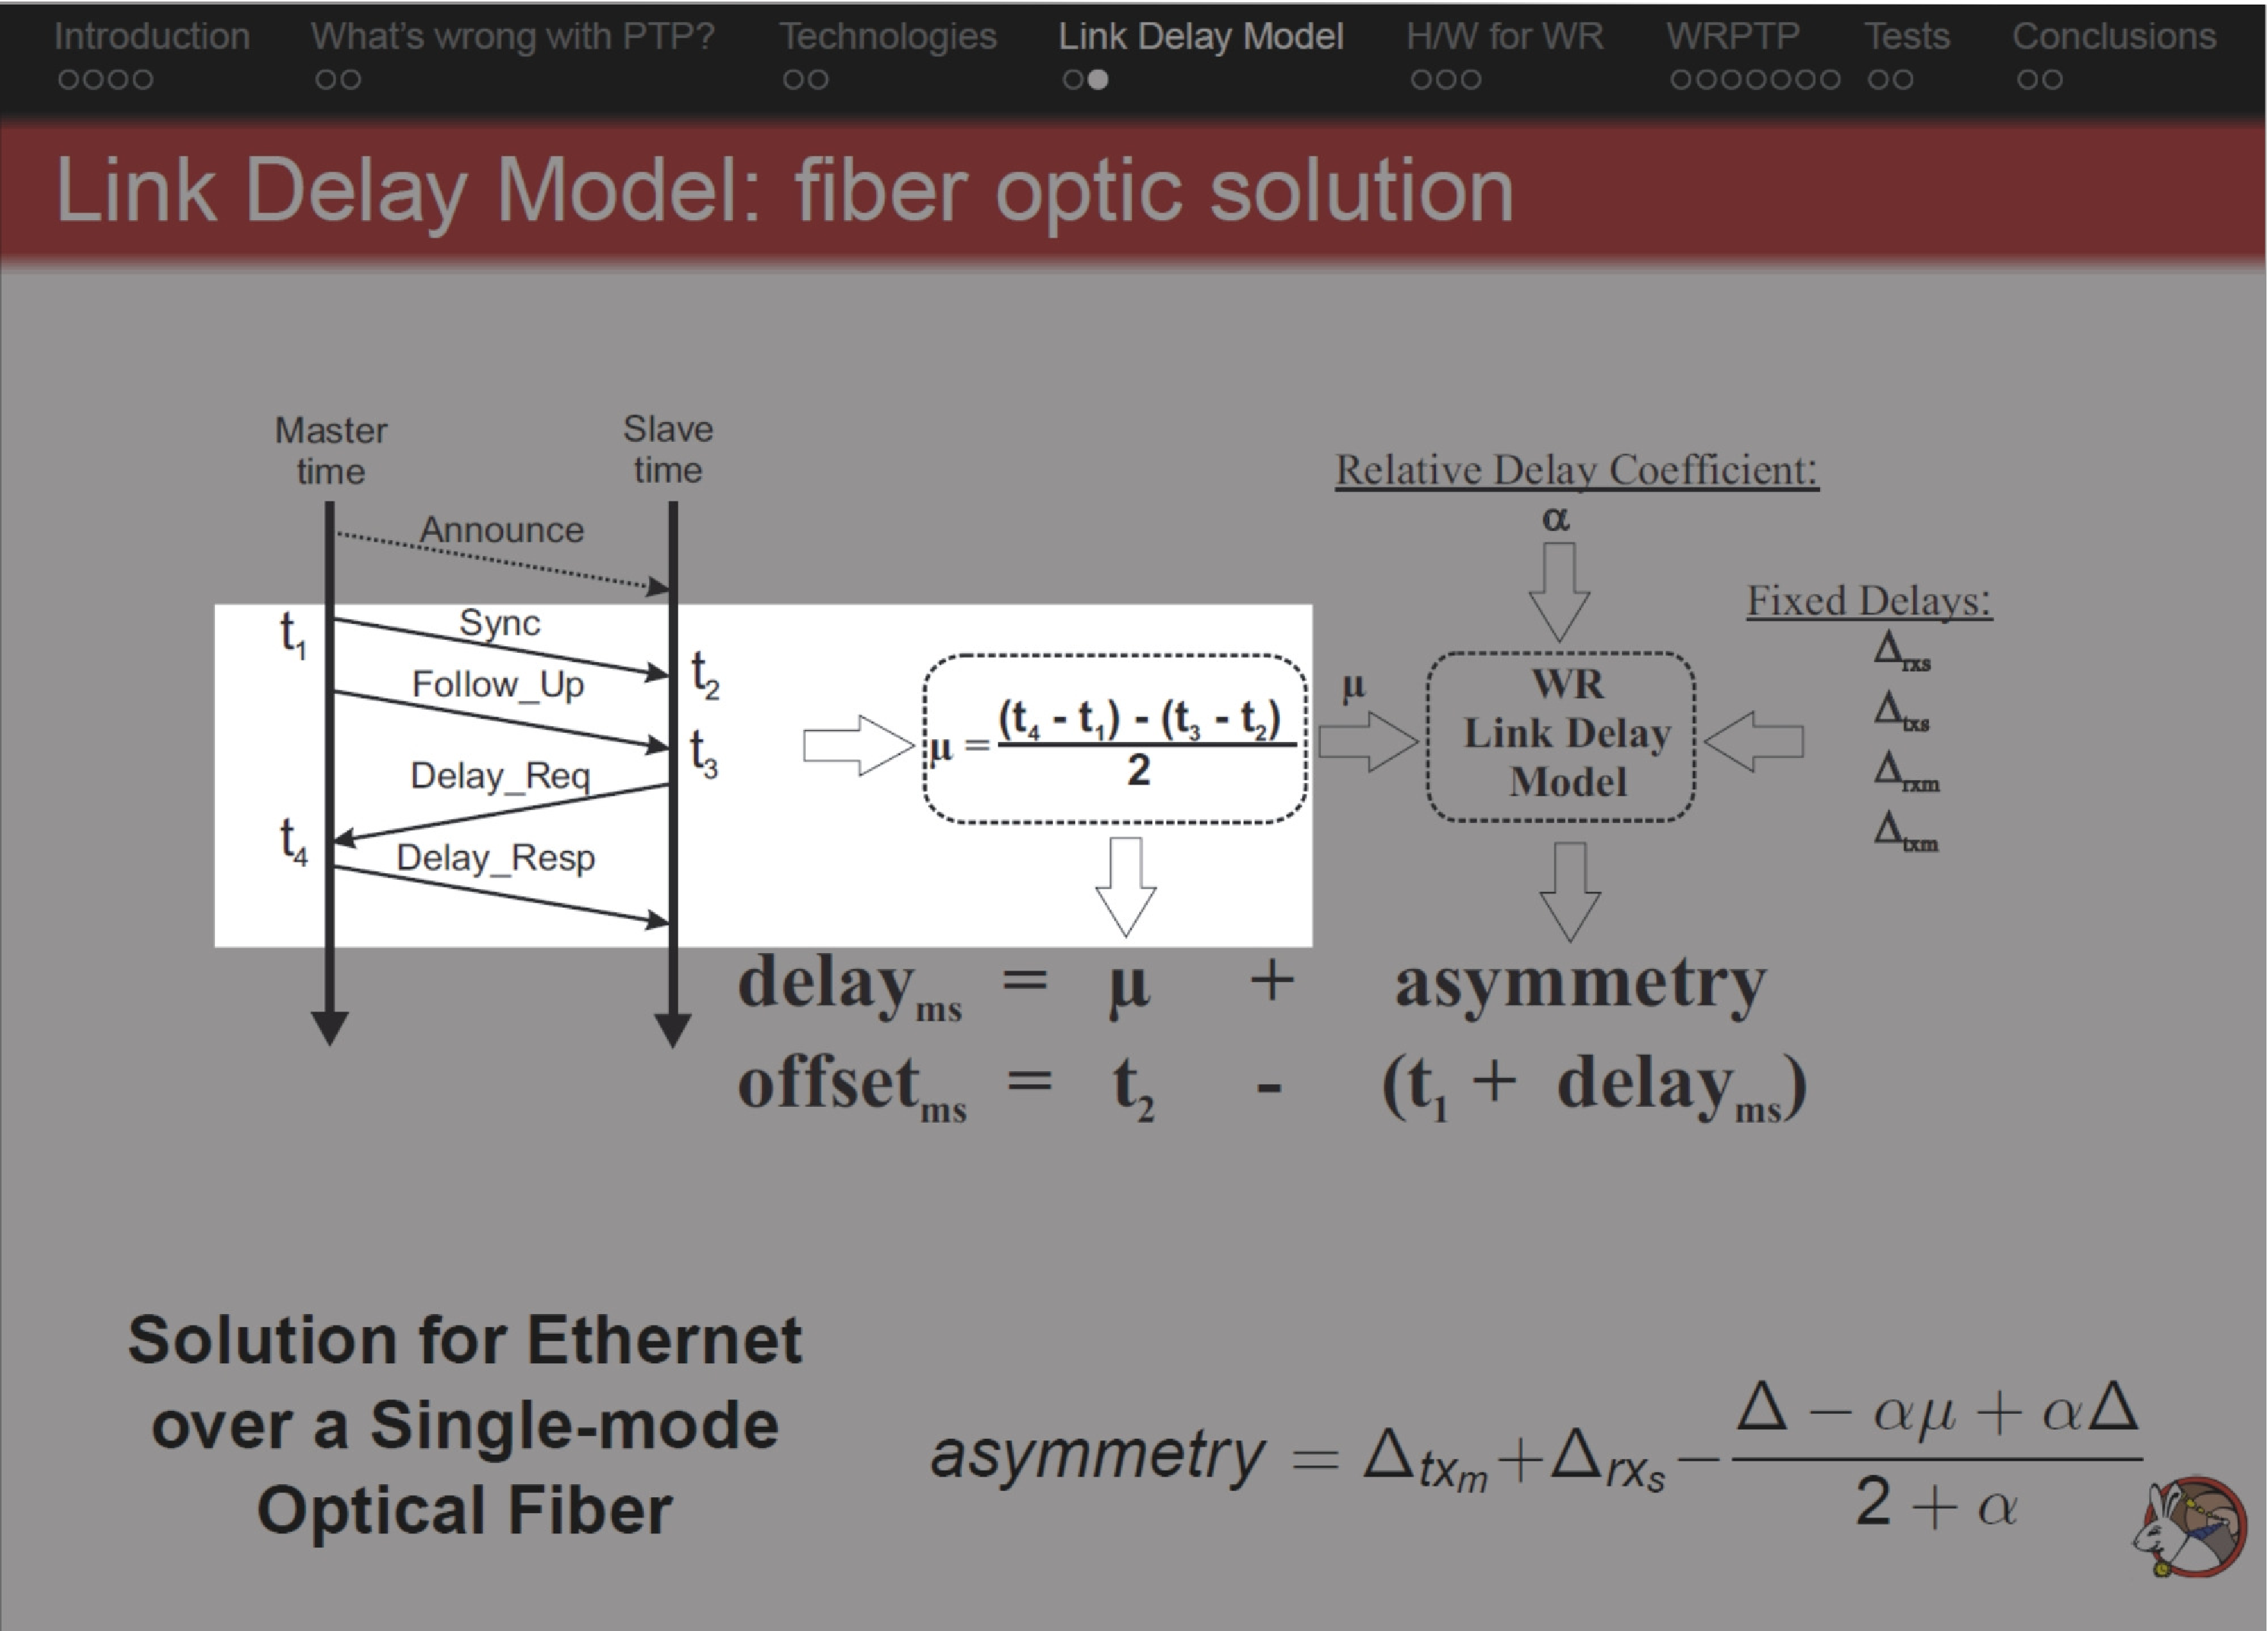
\includegraphics[width=\paperwidth]{protocol/wrLinkModel-fdm2.pdf}}
\logo{}
\begin{frame}{Fine Delay Measurement}

%background

\end{frame}
\setbeamertemplate{background}{} 
\logo{\pgfuseimage{wr-logo}}
%%%%%%%%%%%%%%%%%%%%%%%%%%%%%%%%%%%%%%%%%%%%%%%%%%%%%%%%%%%%%%%%%%%%%%%%%%%%%%%%%%%%%%%%%%%%%%%%%%%%
%\subsection{}
%%%%%%%%%%%%%%%%%%%%%%%%%%%%%%%%%%%%%%%%%%%%%%%%%%%%%%%%%%%%%%%%%%%%%%%%%%%%%%%%%%%%%%%%%%%%%%%%%%%%
\begin{frame}{Fine Delay Measurement}

  \begin{center}
  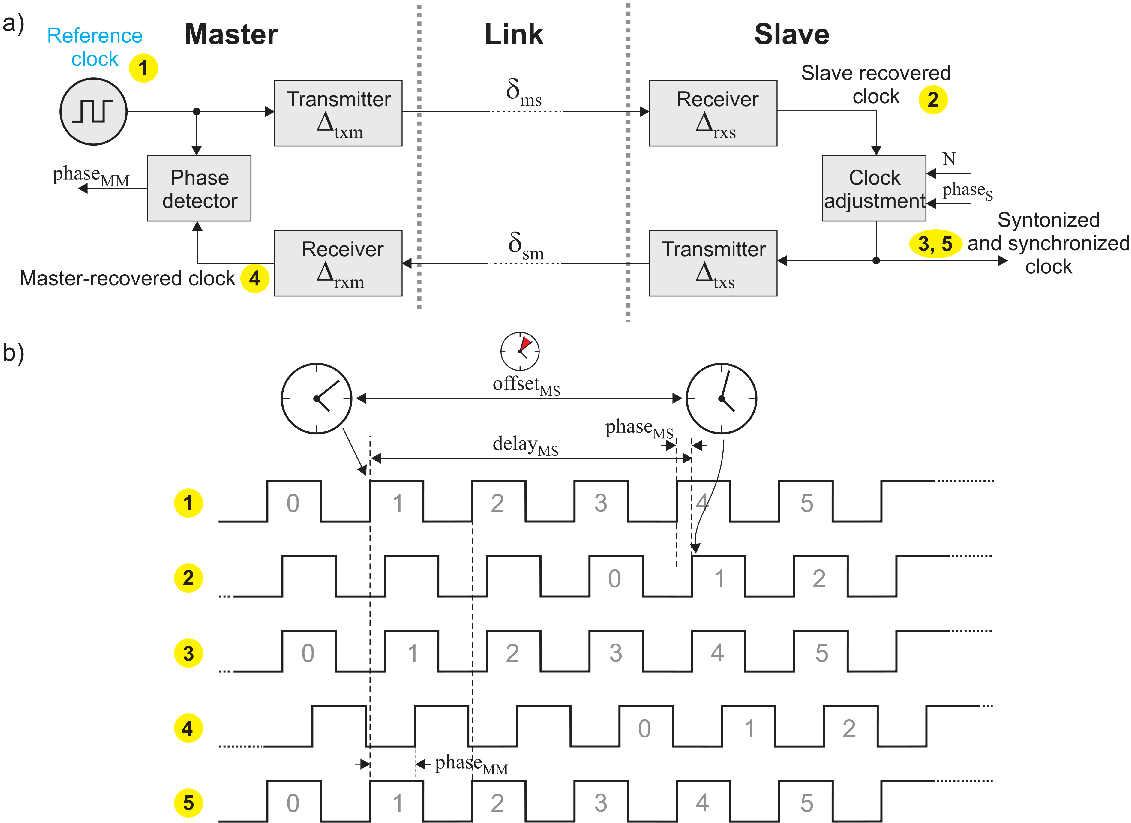
\includegraphics[width=10.0cm]{protocol/link_model.pdf}
  \end{center}

\end{frame}

%%%%%%%%%%%%%%%%%%%%%%%%%%%%%%%%%%%%%%%%%%%%%%%%%%%%%%%%%%%%%%%%%%%%%%%%%%%%%%%%%%%%%%%%%%%%%%%%%%%%
%\subsection{}
%%%%%%%%%%%%%%%%%%%%%%%%%%%%%%%%%%%%%%%%%%%%%%%%%%%%%%%%%%%%%%%%%%%%%%%%%%%%%%%%%%%%%%%%%%%%%%%%%%%%
\setbeamertemplate{background}{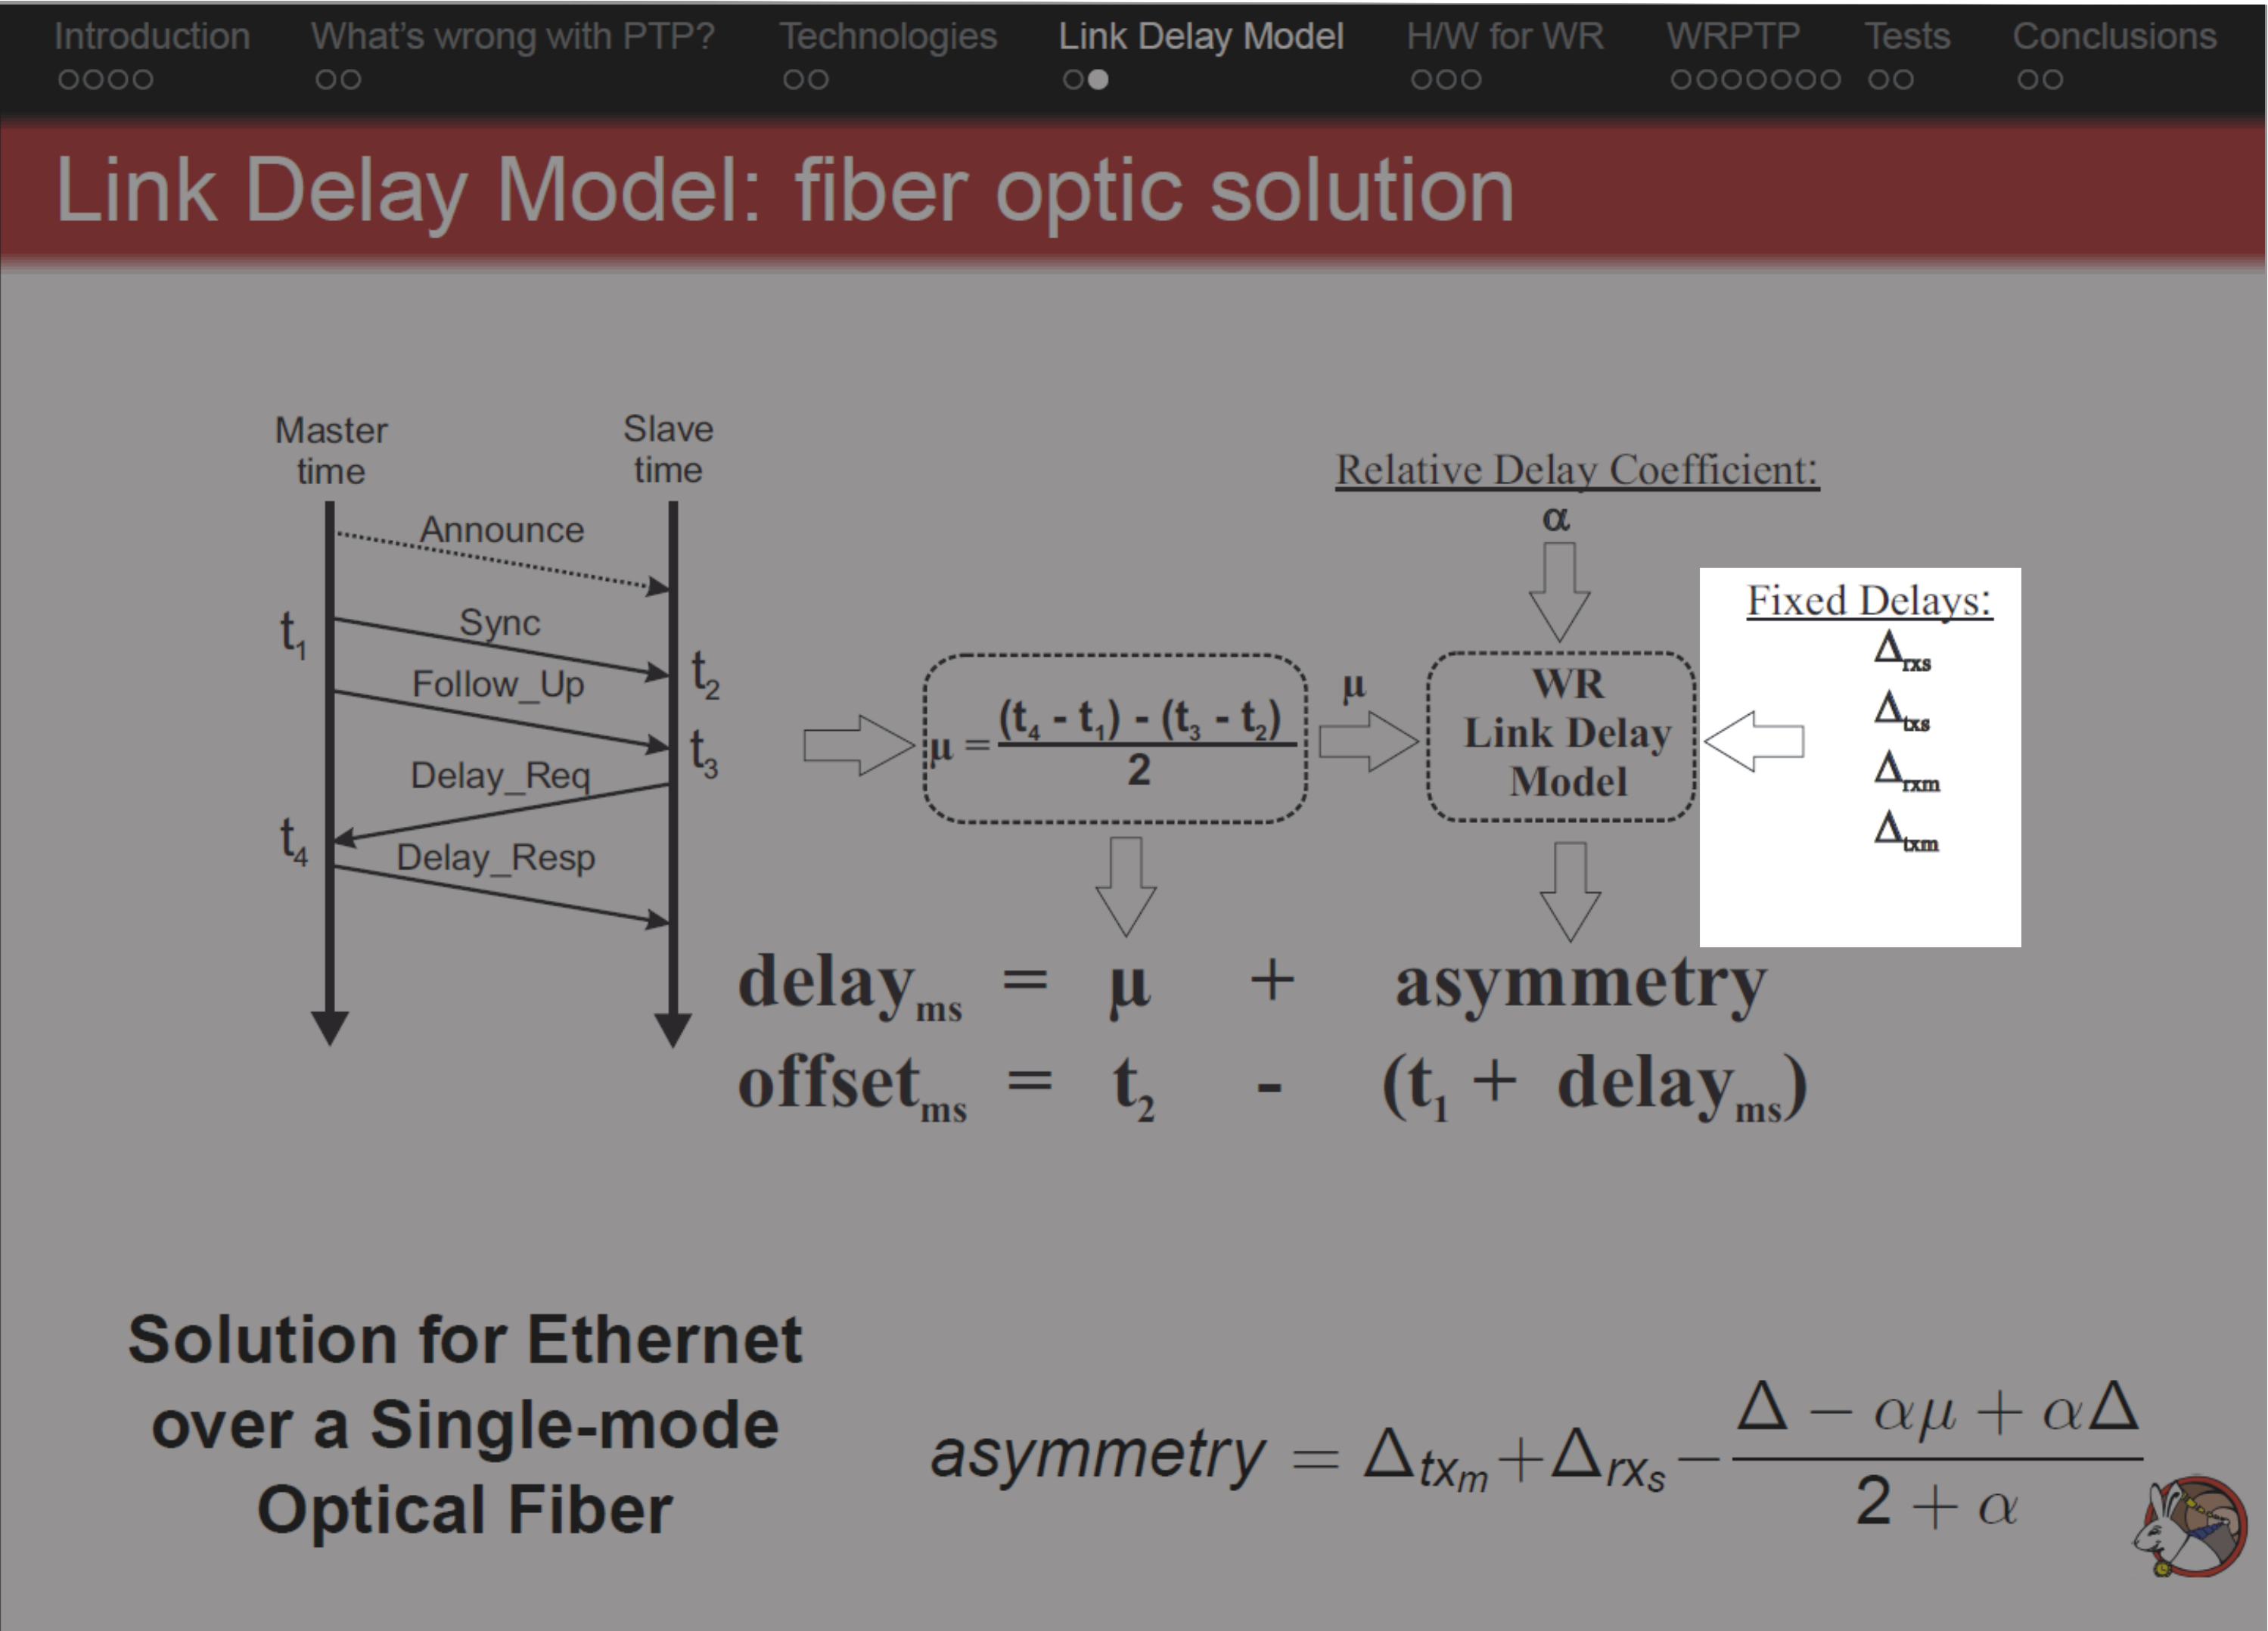
\includegraphics[width=\paperwidth]{protocol/wrLinkModel-fd.pdf}}
\logo{}
\begin{frame}{Fixed Delays Measurement}

%background

\end{frame}
\setbeamertemplate{background}{} 
\logo{\pgfuseimage{wr-logo}}
%%%%%%%%%%%%%%%%%%%%%%%%%%%%%%%%%%%%%%%%%%%%%%%%%%%%%%%%%%%%%%%%%%%%%%%%%%%%%%%%%%%%%%%%%%%%%%%%%%%%
%\subsection{}
%%%%%%%%%%%%%%%%%%%%%%%%%%%%%%%%%%%%%%%%%%%%%%%%%%%%%%%%%%%%%%%%%%%%%%%%%%%%%%%%%%%%%%%%%%%%%%%%%%%%
\begin{frame}{Fixed Delays Measurement}

  \begin{center}
  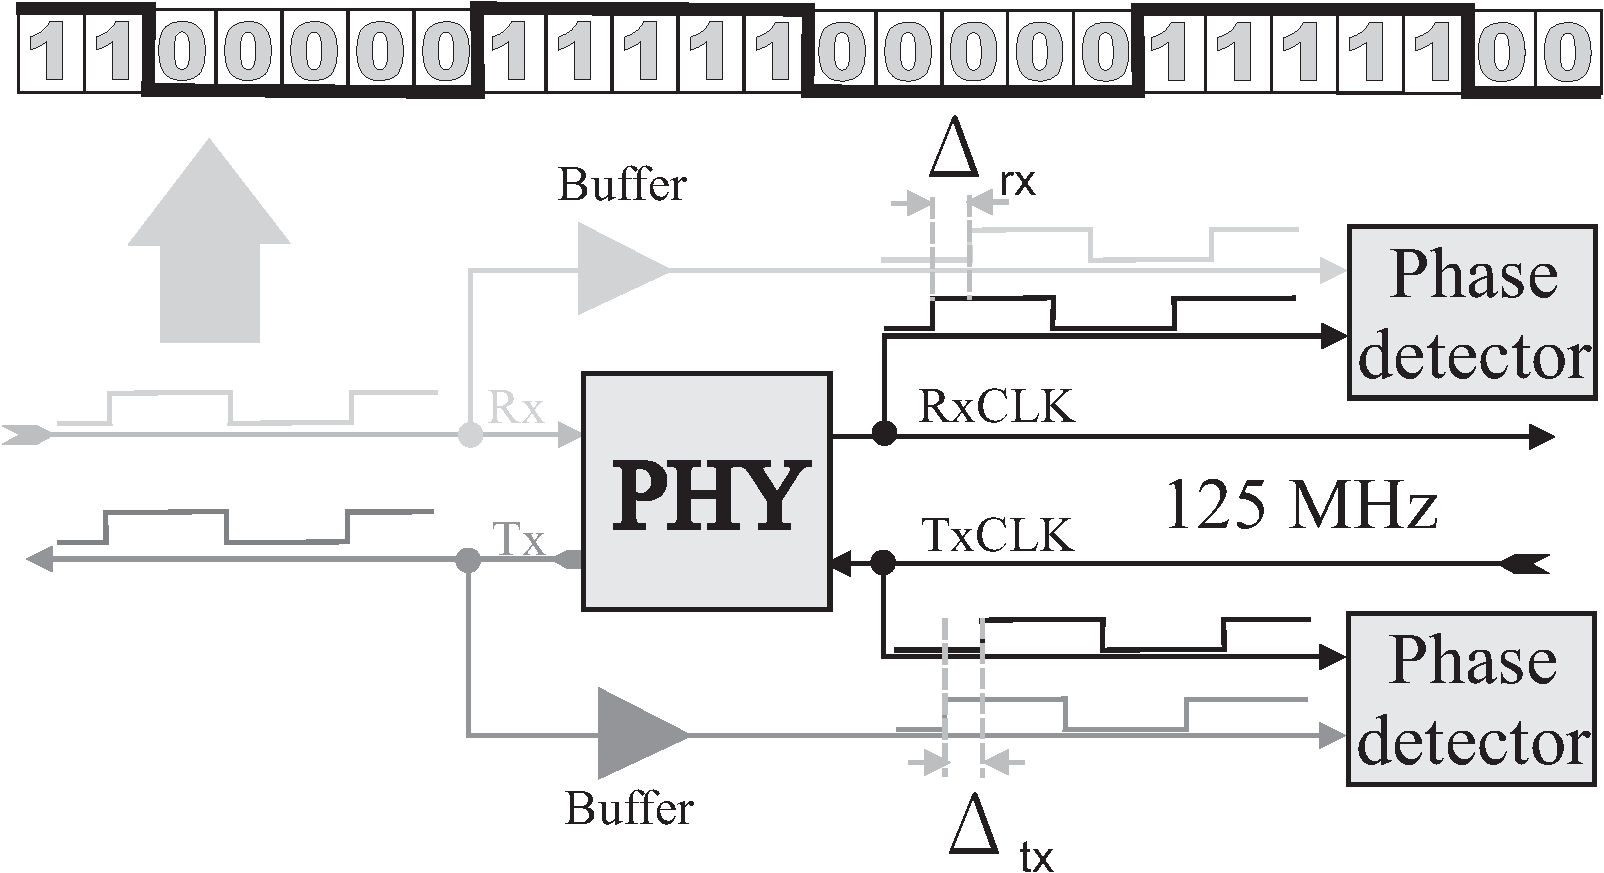
\includegraphics[width=10.0cm]{misc/calibration.pdf}
  \end{center}

\end{frame}
% %%%%%%%%%%%%%%%%%%%%%%%%%%%%%%%%%%%%%%%%%%%%%%%%%%%%%%%%%%%%%%%%%%%%%%%%%%%%%%%%%%%%%%%%%%%%%%%%%%%%
% \subsection{}
% %%%%%%%%%%%%%%%%%%%%%%%%%%%%%%%%%%%%%%%%%%%%%%%%%%%%%%%%%%%%%%%%%%%%%%%%%%%%%%%%%%%%%%%%%%%%%%%%%%%%
% \begin{frame}{Clock Recovery System}
% 
% {\it [problem with a presentation flow]}
% 
%   \begin{center}
%   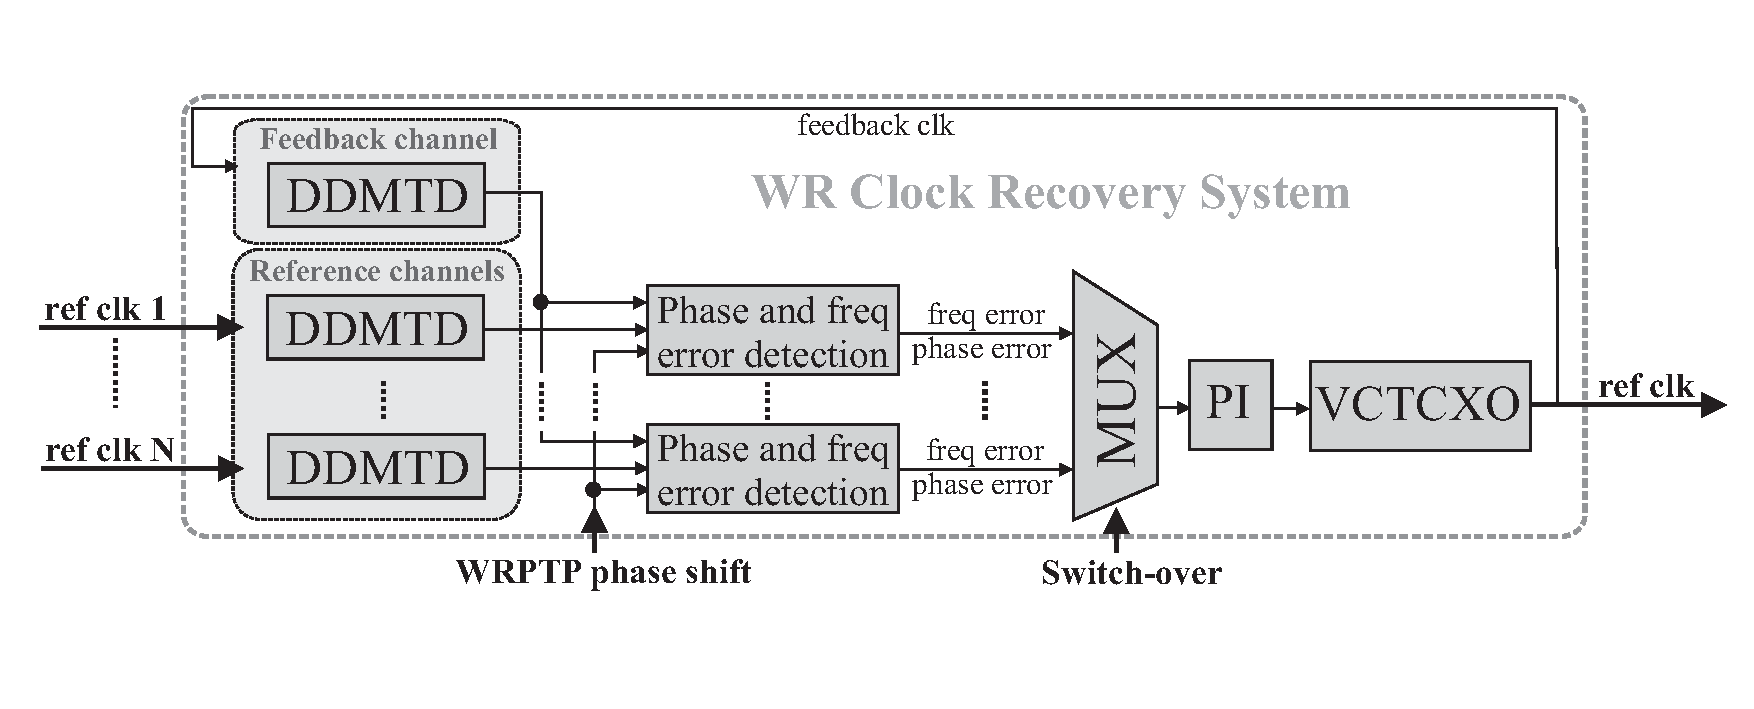
\includegraphics[width=11.5cm]{fig/wrCRS.eps}
%   \end{center}
% 
% \end{frame}
%%%%%%%%%%%%%%%%%%%%%%%%%%%%%%%%%%%%%%%%%%%%%%%%%%%%%%%%%%%%%%%%%%%%%%%%%%%%%%%%%%%%%%%%%%%%%%%%%%%%
%\section{WRPTP}
%\subsection{}
%%%%%%%%%%%%%%%%%%%%%%%%%%%%%%%%%%%%%%%%%%%%%%%%%%%%%%%%%%%%%%%%%%%%%%%%%%%%%%%%%%%%%%%%%%%%%%%%%%%%
\begin{frame}{White Rabbit extension to PTP (WRPTP)}

  \begin{itemize}
    \item Rozpoznanie urządzeń WR
    \item Kalibracja (pomiar $\Delta_{tx_m, rx_m, tx_s, rx_m}$)
    \item Wymiana parametrów WR,
    \item Wsparcie dla nadmiarowości topologii.
  \end{itemize}

\end{frame}
% we need to exchange some extra WR data in order to recognize WR peers (syncE),
% the exchange of data is also needed to perform calibration, where also some extra logic is needed
% and finaly to exchange the WR parameters. Finally, the support of time-source redundancy by 
% the standard PTP is not enough for WR, so we needed to change this as well
%%%%%%%%%%%%%%%%%%%%%%%%%%%%%%%%%%%%%%%%%%%%%%%%%%%%%%%%%%%%%%%%%%%%%%%%%%%%%%%%%%%%%%%%%%%%%%%%%%%%
% \subsection{}
%%%%%%%%%%%%%%%%%%%%%%%%%%%%%%%%%%%%%%%%%%%%%%%%%%%%%%%%%%%%%%%%%%%%%%%%%%%%%%%%%%%%%%%%%%%%%%%%%%%%
% \begin{frame}{Exchange of WR-data}
% 
%   \begin{itemize}
%     \item WR Type-Length-Value (WR TLV):
%       \begin{itemize}
% 	\item tlvType=ORGANIZATION\_EXTENSION
% 	\item OrganizationID=CERN's OUI
%       \end{itemize}
%     \vspace{0.5cm}
%     \item WR data exchange by:
%       \begin{itemize}
% 	\item suffixing Announce Messages
% 	\item creating WR Signaling Messages
%       \end{itemize}
%   \end{itemize}
% 
% \end{frame}
% %%%%%%%%%%%%%%%%%%%%%%%%%%%%%%%%%%%%%%%%%%%%%%%%%%%%%%%%%%%%%%%%%%%%%%%%%%%%%%%%%%%%%%%%%%%%%%%%%%%%
% % \subsection{}
% %%%%%%%%%%%%%%%%%%%%%%%%%%%%%%%%%%%%%%%%%%%%%%%%%%%%%%%%%%%%%%%%%%%%%%%%%%%%%%%%%%%%%%%%%%%%%%%%%%%%
% \begin{frame}{WR-peers recognision}
% 
%   \begin{columns}[c]
%   \column{.5\textwidth} 
% 
%     \begin{center}
%     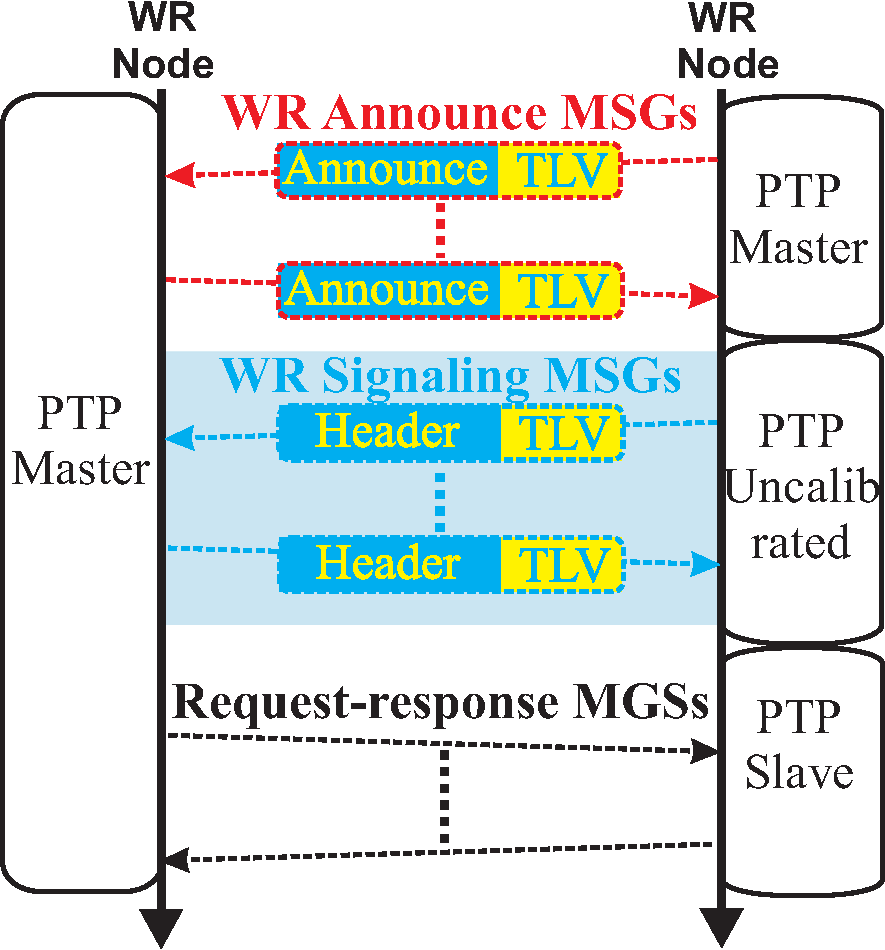
\includegraphics[width=5.5cm]{fig/WR-peer_recognision-1.eps}
%     \end{center}
% 
%   \column{.5\textwidth}
% 
%     \begin{center}
%     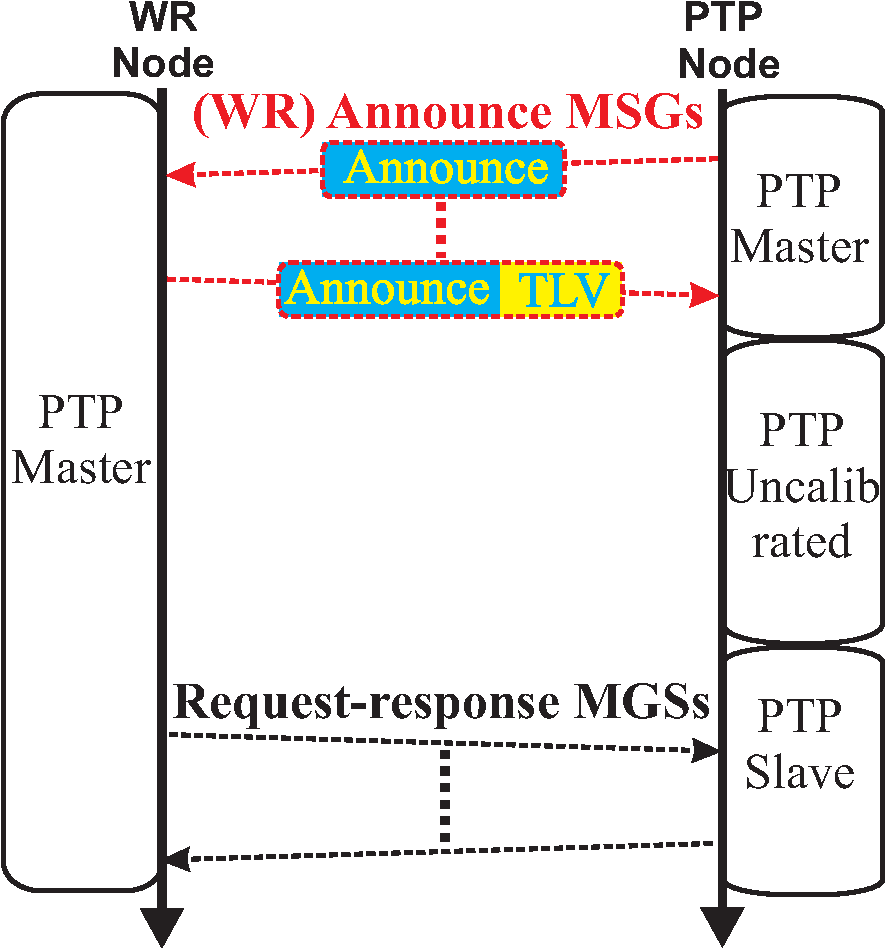
\includegraphics[width=5.5cm]{fig/WR-peer_recognision-2.eps}
%     \end{center}
% 
%   \end{columns}
% 
% \end{frame}
%%%%%%%%%%%%%%%%%%%%%%%%%%%%%%%%%%%%%%%%%%%%%%%%%%%%%%%%%%%%%%%%%%%%%%%%%%%%%%%%%%%%%%%%%%%%%%%%%%%%
% \subsection{}
%%%%%%%%%%%%%%%%%%%%%%%%%%%%%%%%%%%%%%%%%%%%%%%%%%%%%%%%%%%%%%%%%%%%%%%%%%%%%%%%%%%%%%%%%%%%%%%%%%%%
%\begin{frame}{Wymiana parametrów WR}
%
%  \begin{columns}[c]
%  \column{.5\textwidth} 
%
%    \begin{center}
%    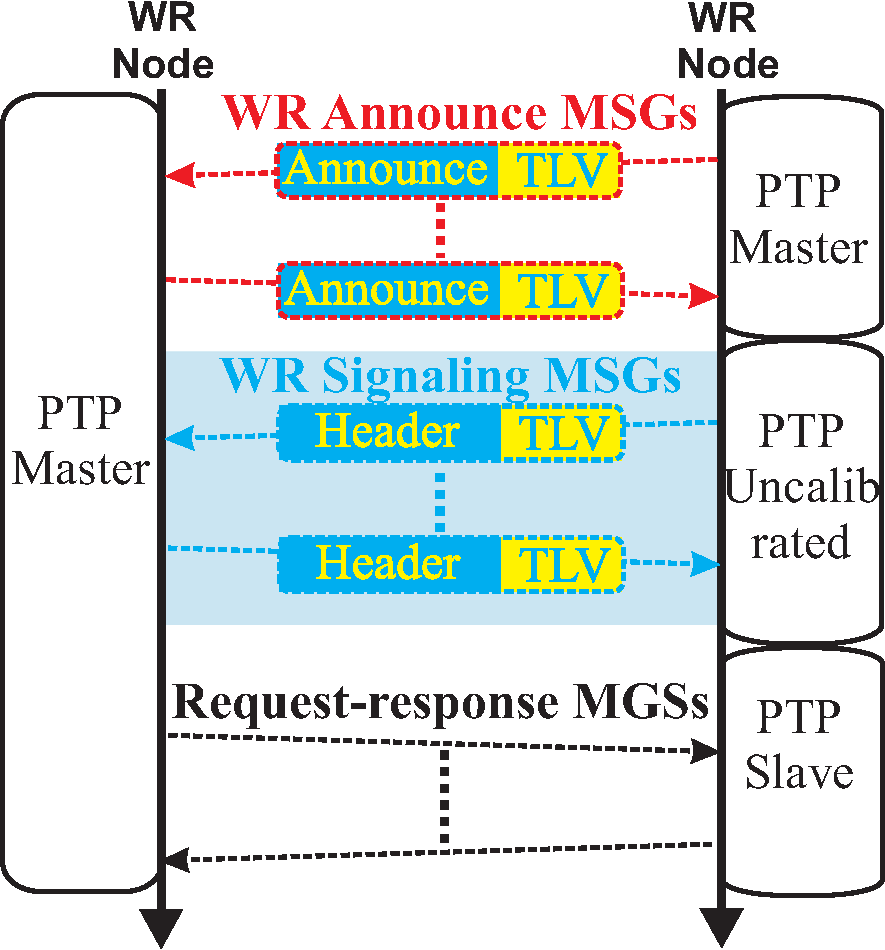
\includegraphics[width=5.5cm]{fig/WR-peer_recognision-1.eps}
%    \end{center}
%
%  \column{.5\textwidth}
%
%    \begin{center}
%    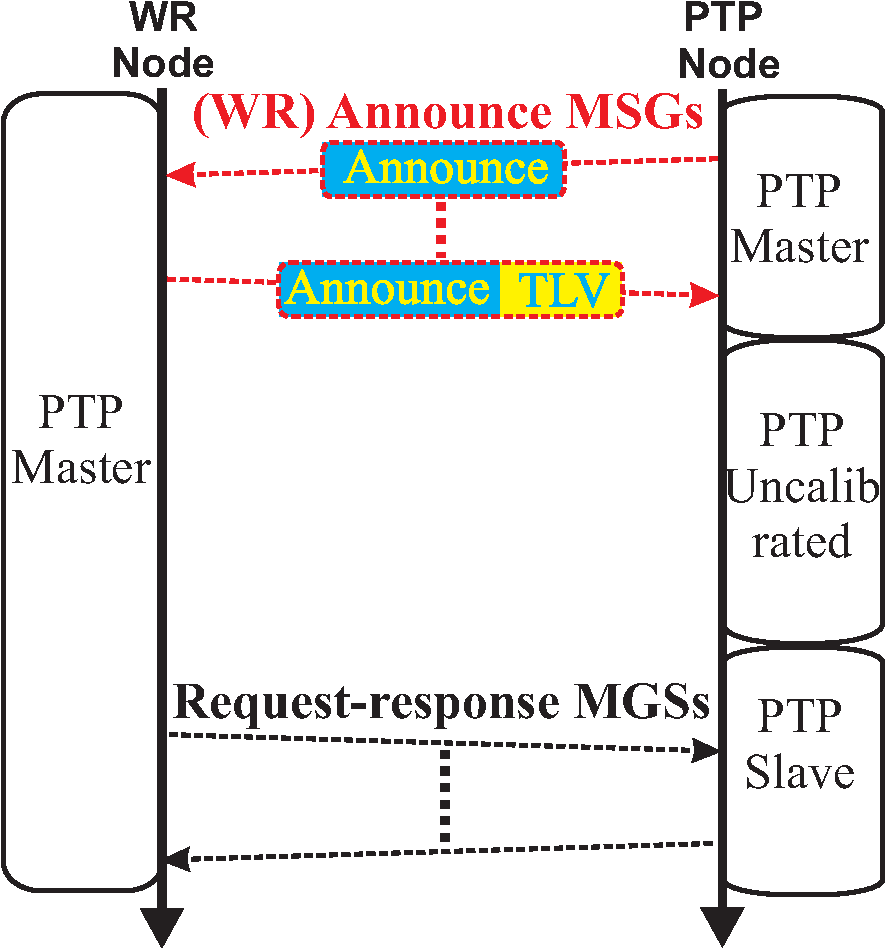
\includegraphics[width=5.5cm]{fig/WR-peer_recognision-2.eps}
%    \end{center}
%
%  \end{columns}
%
%\end{frame}
%%%%%%%%%%%%%%%%%%%%%%%%%%%%%%%%%%%%%%%%%%%%%%%%%%%%%%%%%%%%%%%%%%%%%%%%%%%%%%%%%%%%%%%%%%%%%%%%%%%%
% \subsection{}
%%%%%%%%%%%%%%%%%%%%%%%%%%%%%%%%%%%%%%%%%%%%%%%%%%%%%%%%%%%%%%%%%%%%%%%%%%%%%%%%%%%%%%%%%%%%%%%%%%%%
\begin{frame}{WR Link Setup }

  \begin{columns}[c]
  \column{.5\textwidth} 

      \begin{center}
      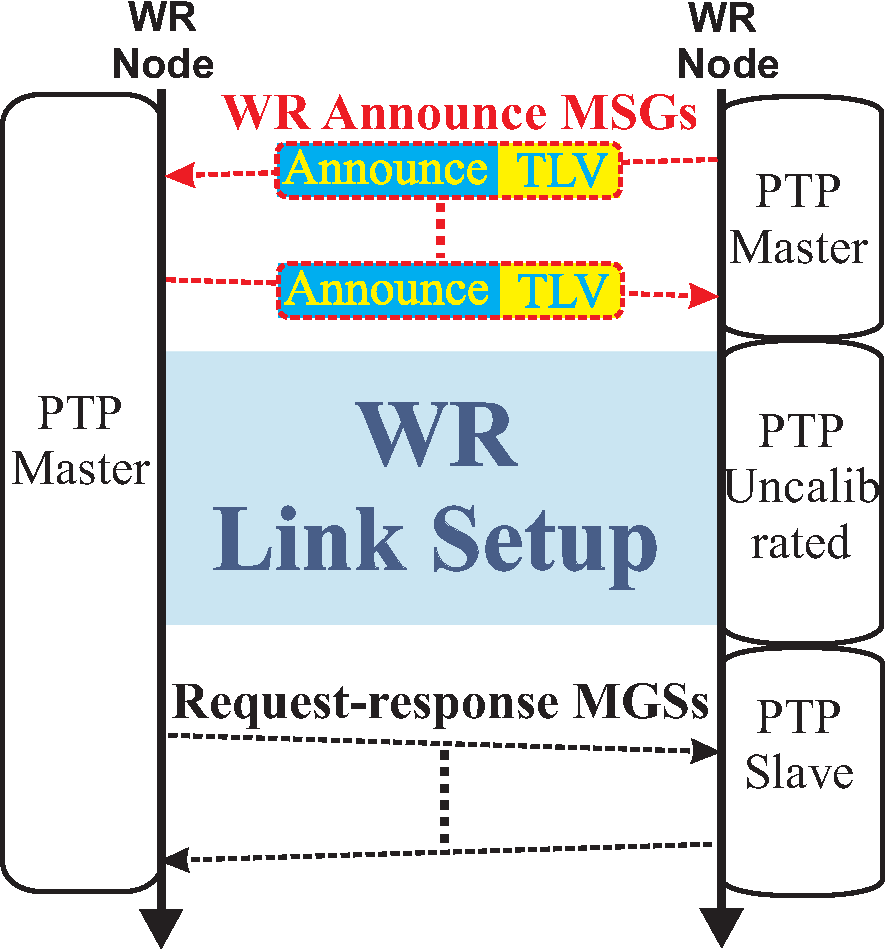
\includegraphics[width=5.5cm]{protocol/wrLinkSetup.pdf}
      \end{center}


  \column{.5\textwidth} 

      \begin{itemize}
	\item Dostrojenie częstotliwości (syntonizacja)
	\item Kalibracja
	\item Wymiana parametrów WR
	\item WR Finite State Machine (FSM)
	\item WR Signaling Messages
      \end{itemize}

  \end{columns}

\end{frame}
%%%%%%%%%%%%%%%%%%%%%%%%%%%%%%%%%%%%%%%%%%%%%%%%%%%%%%%%%%%%%%%%%%%%%%%%%%%%%%%%%%%%%%%%%%%%%%%%%%%%
% \subsection{}
%%%%%%%%%%%%%%%%%%%%%%%%%%%%%%%%%%%%%%%%%%%%%%%%%%%%%%%%%%%%%%%%%%%%%%%%%%%%%%%%%%%%%%%%%%%%%%%%%%%%
% \begin{frame}{WR Link Setup}
% 
%       \begin{center}
%       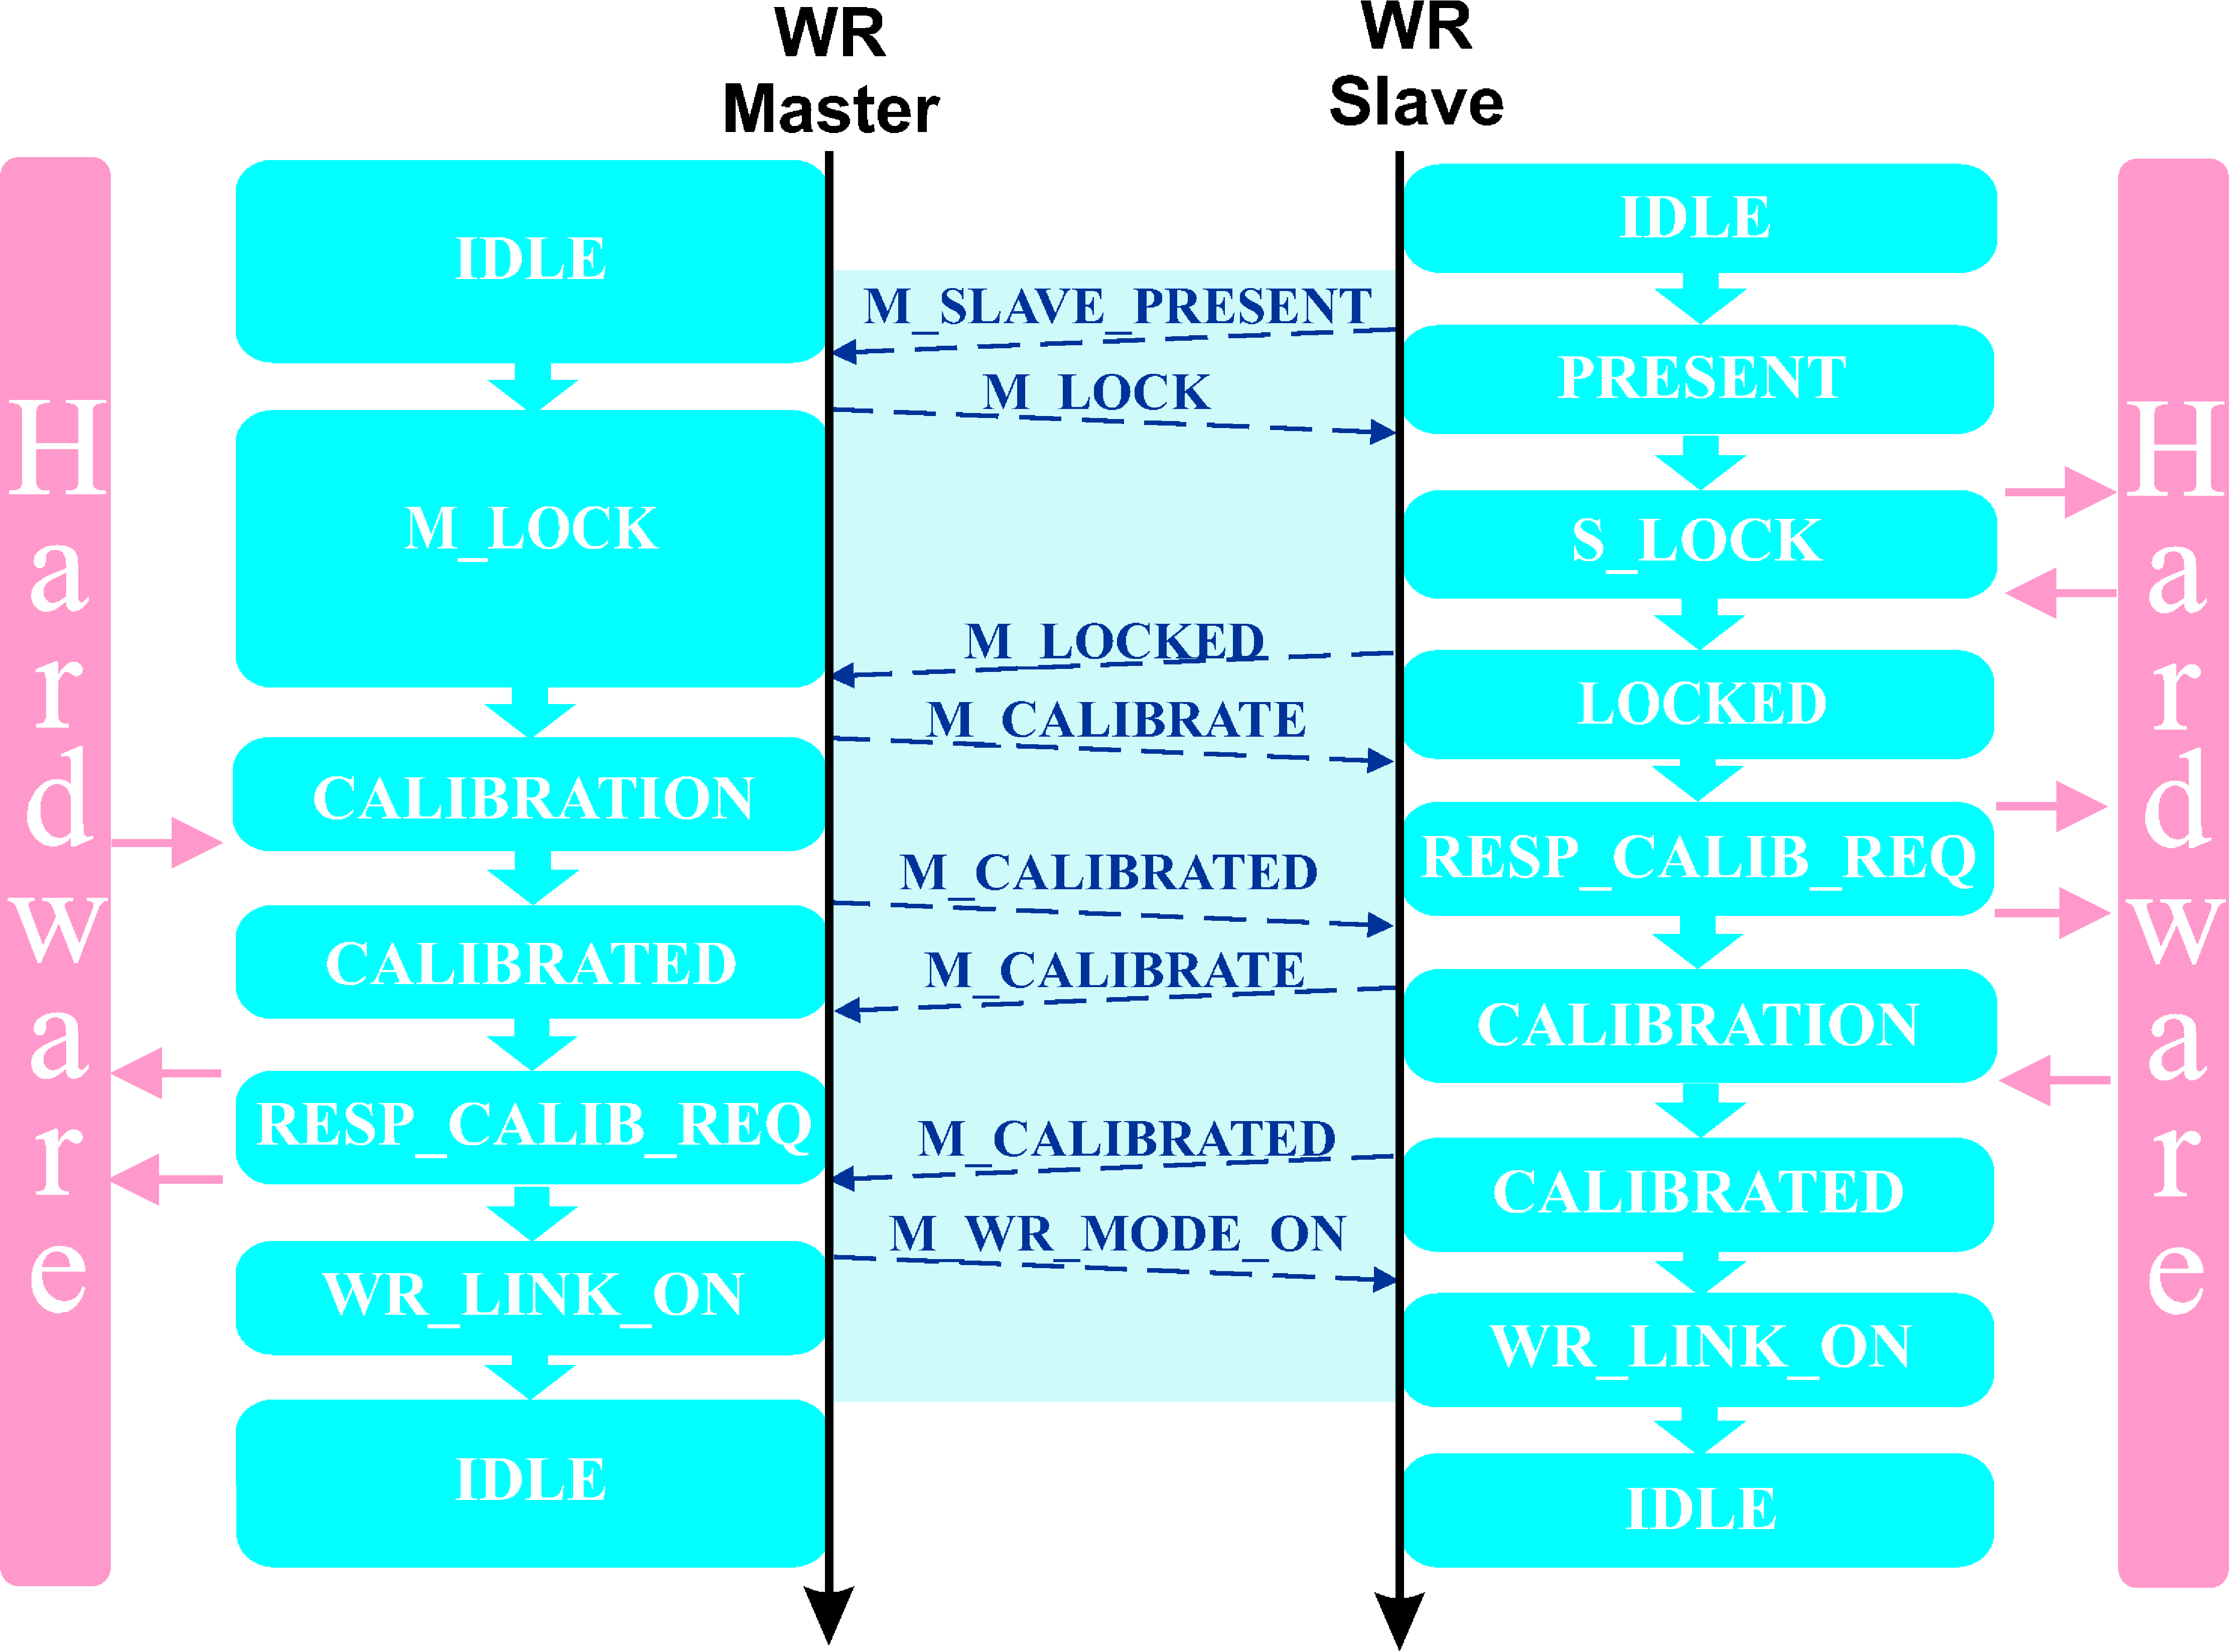
\includegraphics[width=9.5cm]{fig/wrLinkSetupFSM.eps}
%       \end{center}
% 
% \end{frame}
%%%%%%%%%%%%%%%%%%%%%%%%%%%%%%%%%%%%%%%%%%%%%%%%%%%%%%%%%%%%%%%%%%%%%%%%%%%%%%%%%%%%%%%%%%%%%%%%%%%%
% \subsection{}
%%%%%%%%%%%%%%%%%%%%%%%%%%%%%%%%%%%%%%%%%%%%%%%%%%%%%%%%%%%%%%%%%%%%%%%%%%%%%%%%%%%%%%%%%%%%%%%%%%%%
% \begin{frame}{Redundancy: BMC}
% 
% \begin{columns}[c]
% \column{.6\textwidth} 
%     \begin{itemize}
% 	\item disjoint logic trees for multiple \textit{best} clocks,
% 	\item redundancy not optimal for the continuity of the synchronization,
% 	\item no more than one PTP SLAVE port in a single Boundary Clock.
%       \end{itemize}
% {\it[correct spelling of GPS in fig]}
% \column{.4\textwidth}
%     \begin{center}
%     \includegraphics[height=7.0cm]{fig/BMC.eps}
%      \end{center}
% \end{columns}
% 
% 
% \end{frame}
%%%%%%%%%%%%%%%%%%%%%%%%%%%%%%%%%%%%%%%%%%%%%%%%%%%%%%%%%%%%%%%%%%%%%%%%%%%%%%%%%%%%%%%%%%%%%%%%%%%%
% \subsection{}
%%%%%%%%%%%%%%%%%%%%%%%%%%%%%%%%%%%%%%%%%%%%%%%%%%%%%%%%%%%%%%%%%%%%%%%%%%%%%%%%%%%%%%%%%%%%%%%%%%%%
% \begin{frame}{Redundancy: modified BMC}
% 
% \begin{columns}[c]
% \column{.6\textwidth}
% 
%     \begin{block}{Modified BMC}
%     ... forces PTP\_SLAVE state instead of PTP\_PASSIVE for clockClass $>$ 127
%     \end{block}
% 
%     \begin{itemize}
% 	\item Many PTP SLAVE ports in a single Boundary Clock,
% 	\item Active PTP SLAVE port used to synchronize and syntonize local clock.
% 	\item Modifies State Decision Algorithm.
% 	\item New Data Fields update. 
%       \end{itemize}
% {\it[correct spelling of GPS in fig]}
% \column{.4\textwidth}
%     \begin{center}
%     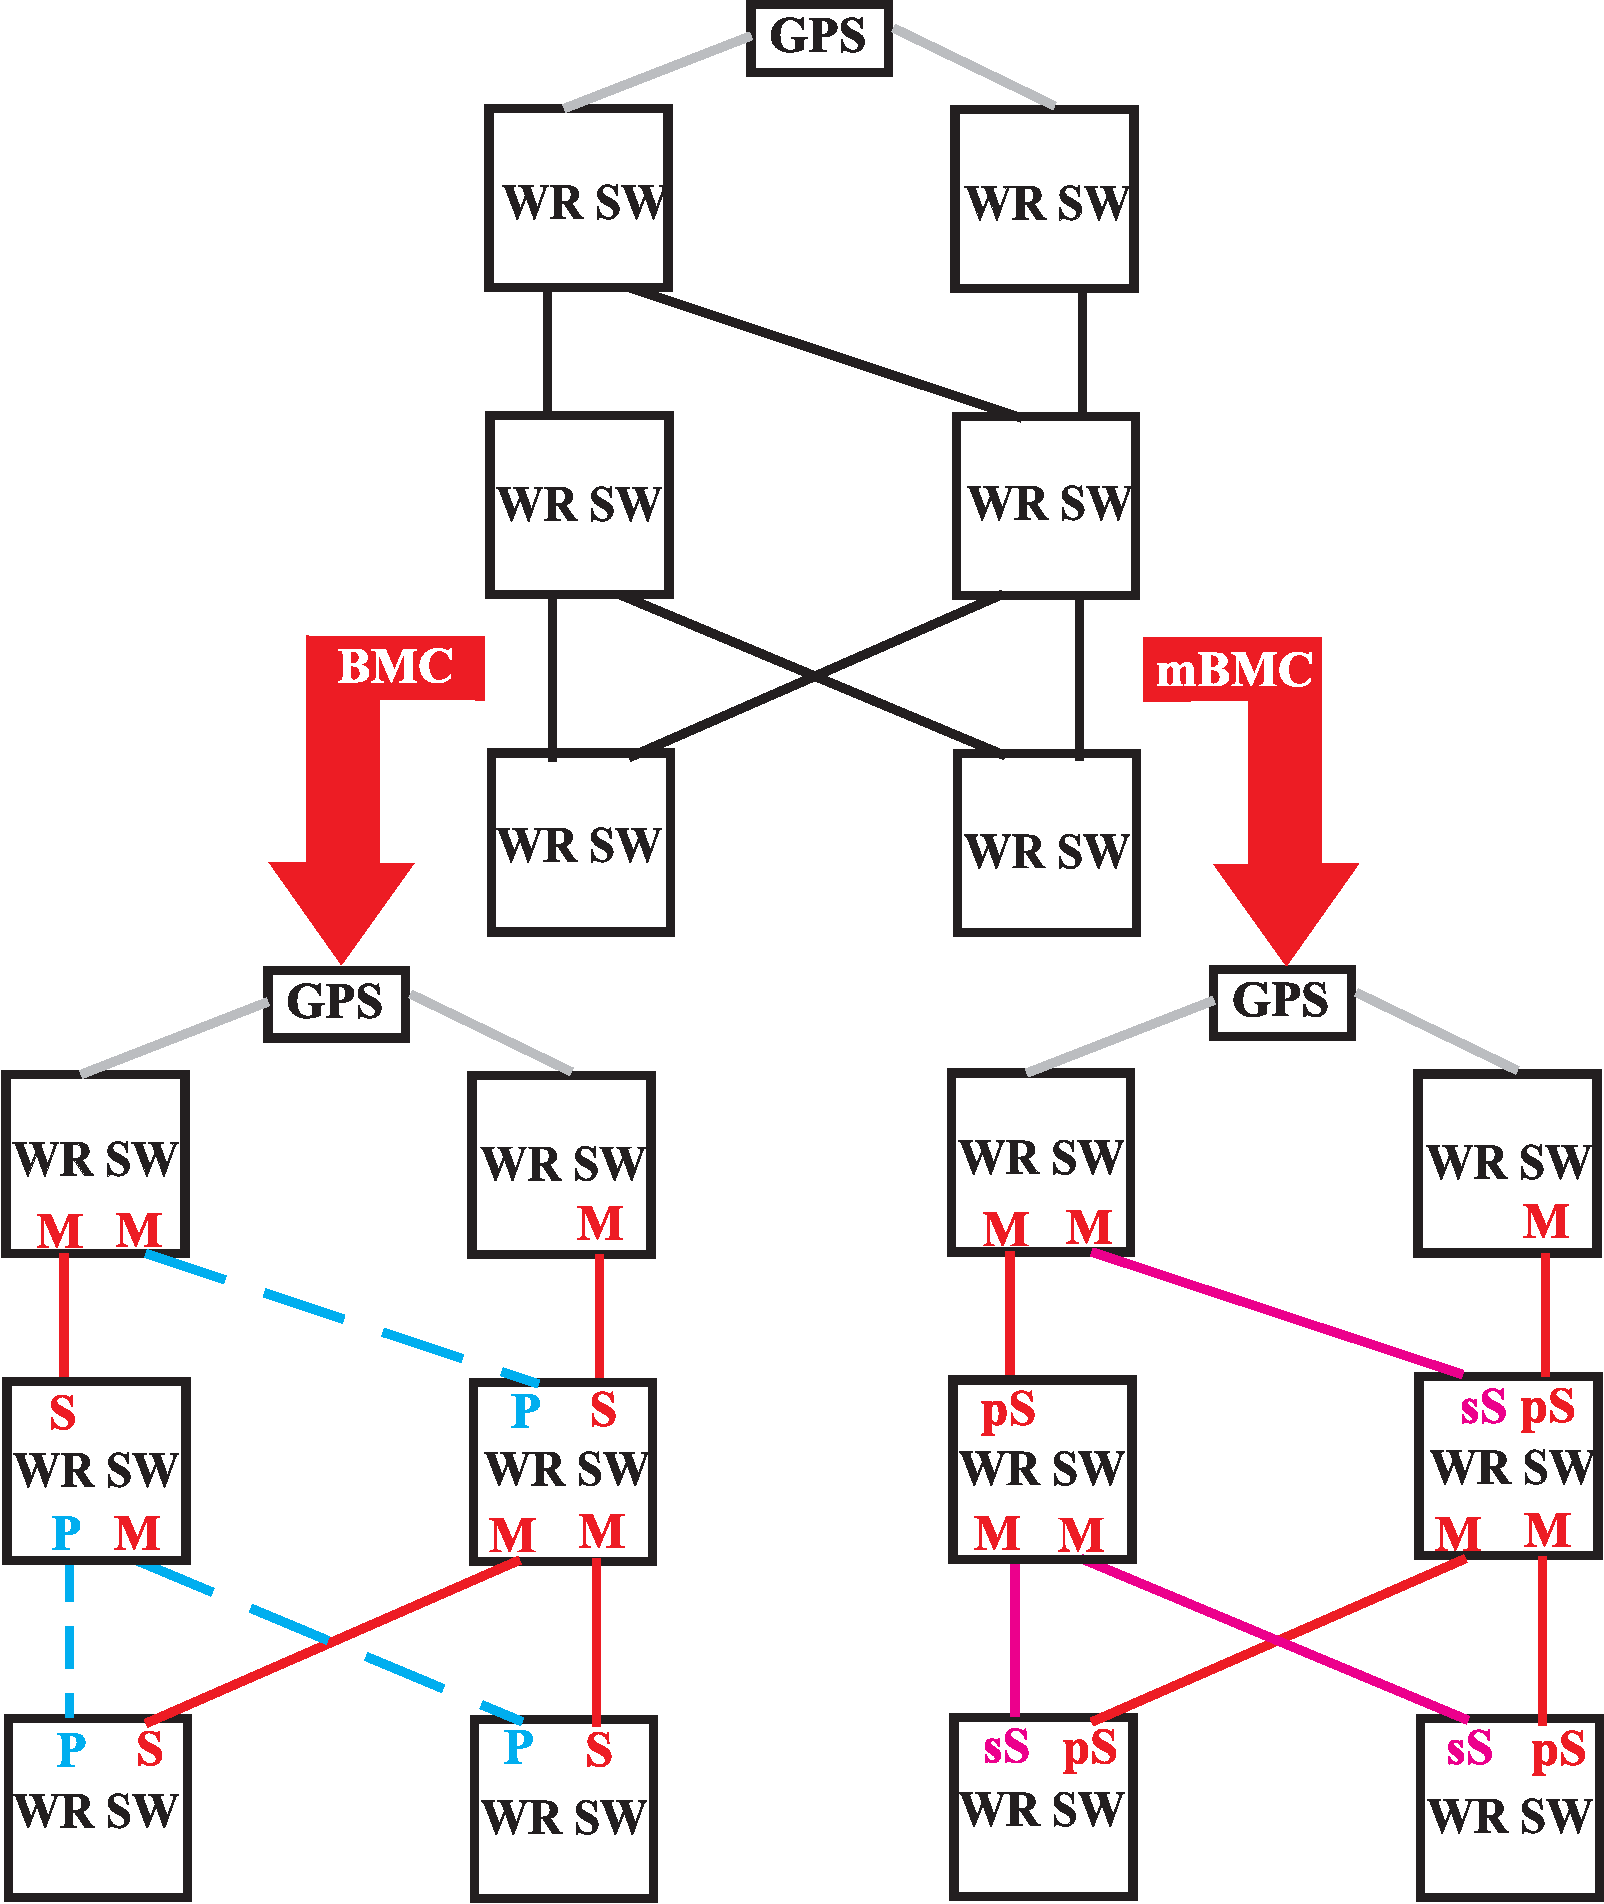
\includegraphics[height=7.0cm]{fig/mBMCvsBMC.eps}
%     \end{center}
% \end{columns}
% 
% \end{frame}
%%%%%%%%%%%%%%%%%%%%%%%%%%%%%%%%%%%%%%%%%%%%%%%%%%%%%%%%%%%%%%%%%%%%%%%%%%%%%%%%%%%%%%%%%%%%%%%%%%%%
% \section{H/W for WR}
% \subsection{H/W for WR}
%%%%%%%%%%%%%%%%%%%%%%%%%%%%%%%%%%%%%%%%%%%%%%%%%%%%%%%%%%%%%%%%%%%%%%%%%%%%%%%%%%%%%%%%%%%%%%%%%%%%
\begin{frame}{Wsparcie dla nadmiarowości sieci}

%{\it [problem with a presentation flow]}

  \begin{center}
  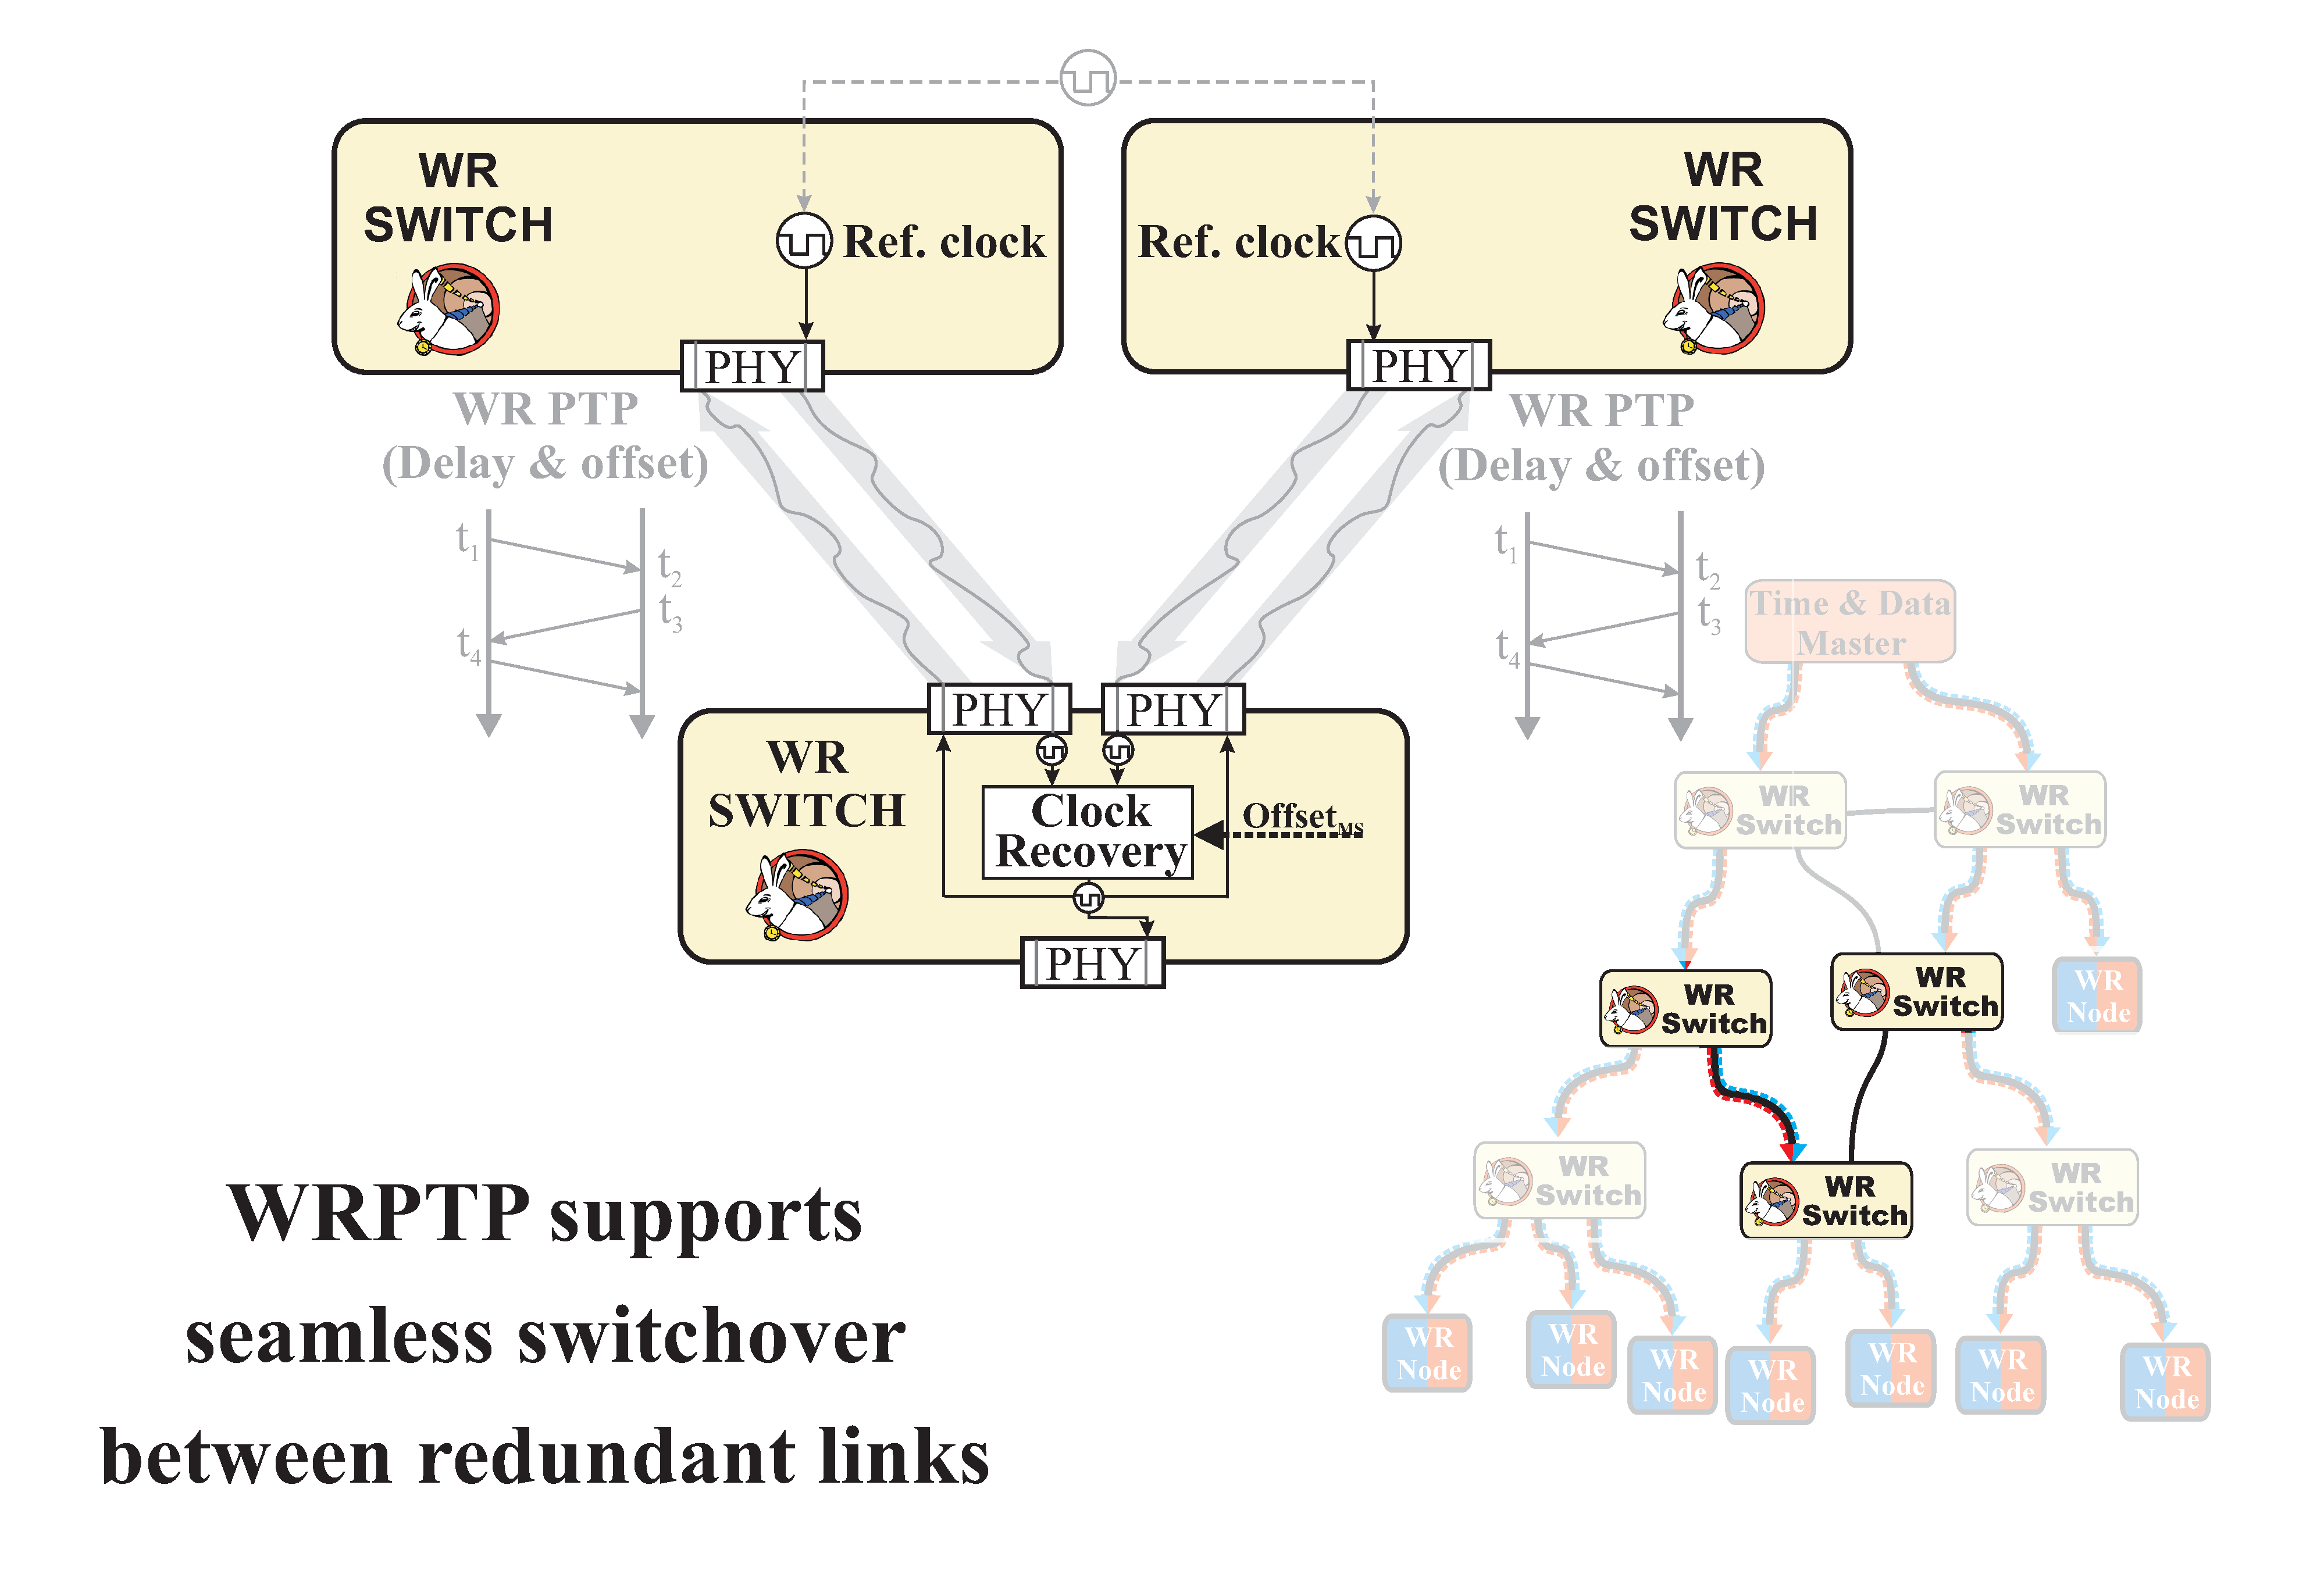
\includegraphics[width=10cm]{robustness/wrCRS2.pdf}
  \end{center}

\end{frame}
%%%%%%%%%%%%%%%%%%%%%%%%%%%%%%%%%%%%%%%%%%%%%%%%%%%%%%%%%%%%%%%%%%%%%%%%%%%%%%%%%%%%%%%%%%%%%%%%%%%%
% \section{H/W for WR}
% \subsection{H/W for WR}
%%%%%%%%%%%%%%%%%%%%%%%%%%%%%%%%%%%%%%%%%%%%%%%%%%%%%%%%%%%%%%%%%%%%%%%%%%%%%%%%%%%%%%%%%%%%%%%%%%%%
\begin{frame}{Wsparcie dla nadmiarowości sieci}

%{\it [problem with a presentation flow]}

  \begin{center}
  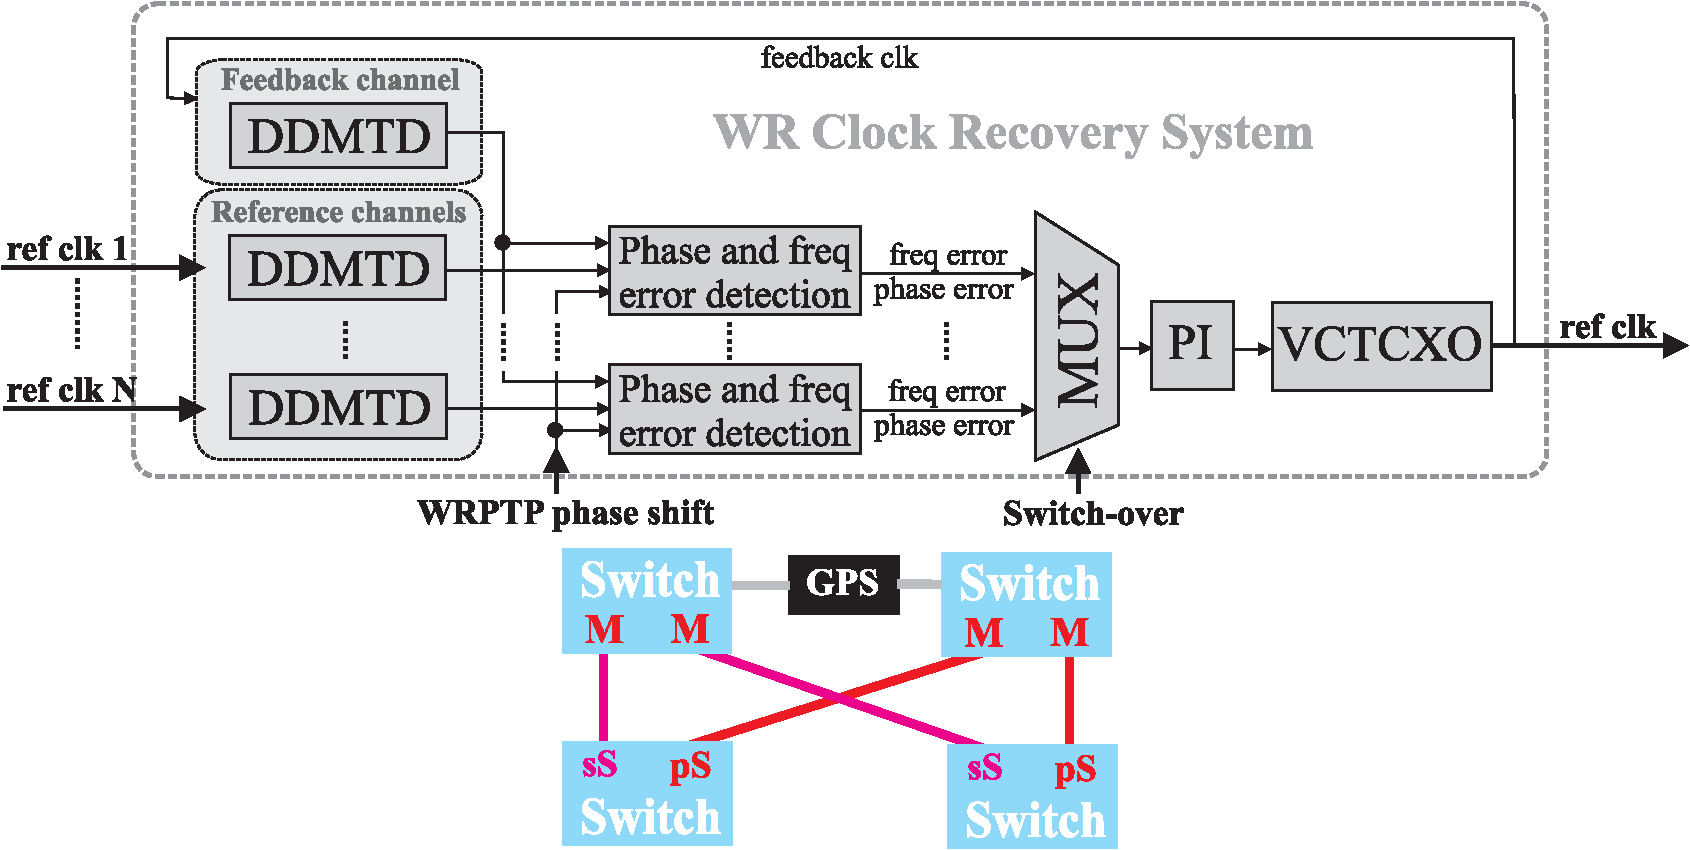
\includegraphics[width=11.8cm]{protocol/wrCRS_plus_mBMC.pdf}
  \end{center}

\end{frame}
%%%%%%%%%%%%%%%%%%%%%%%%%%%%%%%%%%%%%%%%%%%%%%%%%%%%%%%%%%%%%%%%%%%%%%%%%%%%%%%%%%%%%%%%%%%%%%%%%%%%
%\section{Status}
%\subsection{}
%%%%%%%%%%%%%%%%%%%%%%%%%%%%%%%%%%%%%%%%%%%%%%%%%%%%%%%%%%%%%%%%%%%%%%%%%%%%%%%%%%%%%%%%%%%%%%%%%%%%
\begin{frame}{Testy: synchronizacja w układzie kaskadowym}

    \begin{center}
    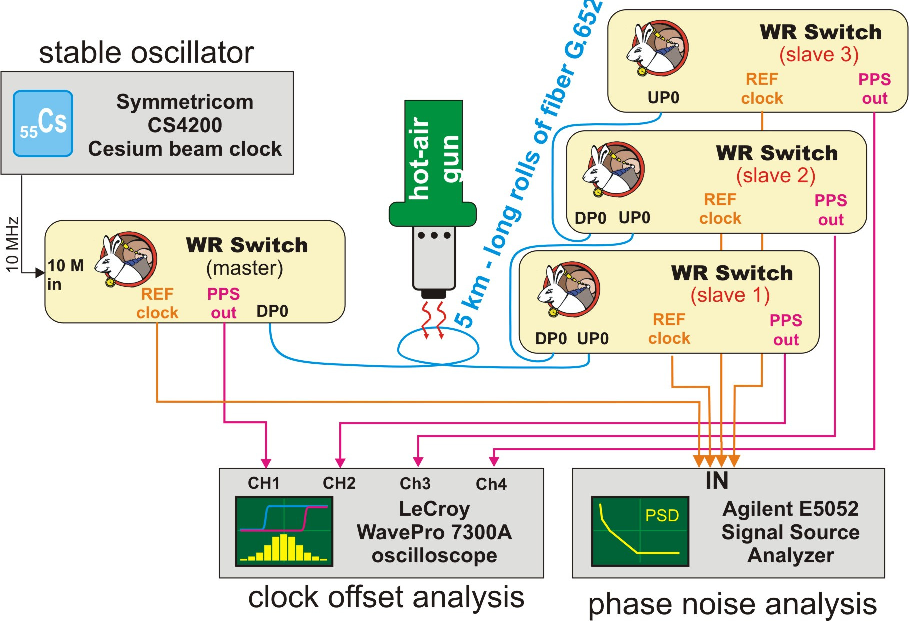
\includegraphics[height=7.0cm]{measurements/measSystem.pdf}
    \end{center}

\end{frame}
%%%%%%%%%%%%%%%%%%%%%%%%%%%%%%%%%%%%%%%%%%%%%%%%%%%%%%%%%%%%%%%%%%%%%%%%%%%%%%%%%%%%%%%%%%%%%%%%%%%%
% \subsection{}
%%%%%%%%%%%%%%%%%%%%%%%%%%%%%%%%%%%%%%%%%%%%%%%%%%%%%%%%%%%%%%%%%%%%%%%%%%%%%%%%%%%%%%%%%%%%%%%%%%%%
\begin{frame}{Testy: synchronizacja w układzie kaskadowym}

    \begin{center}
    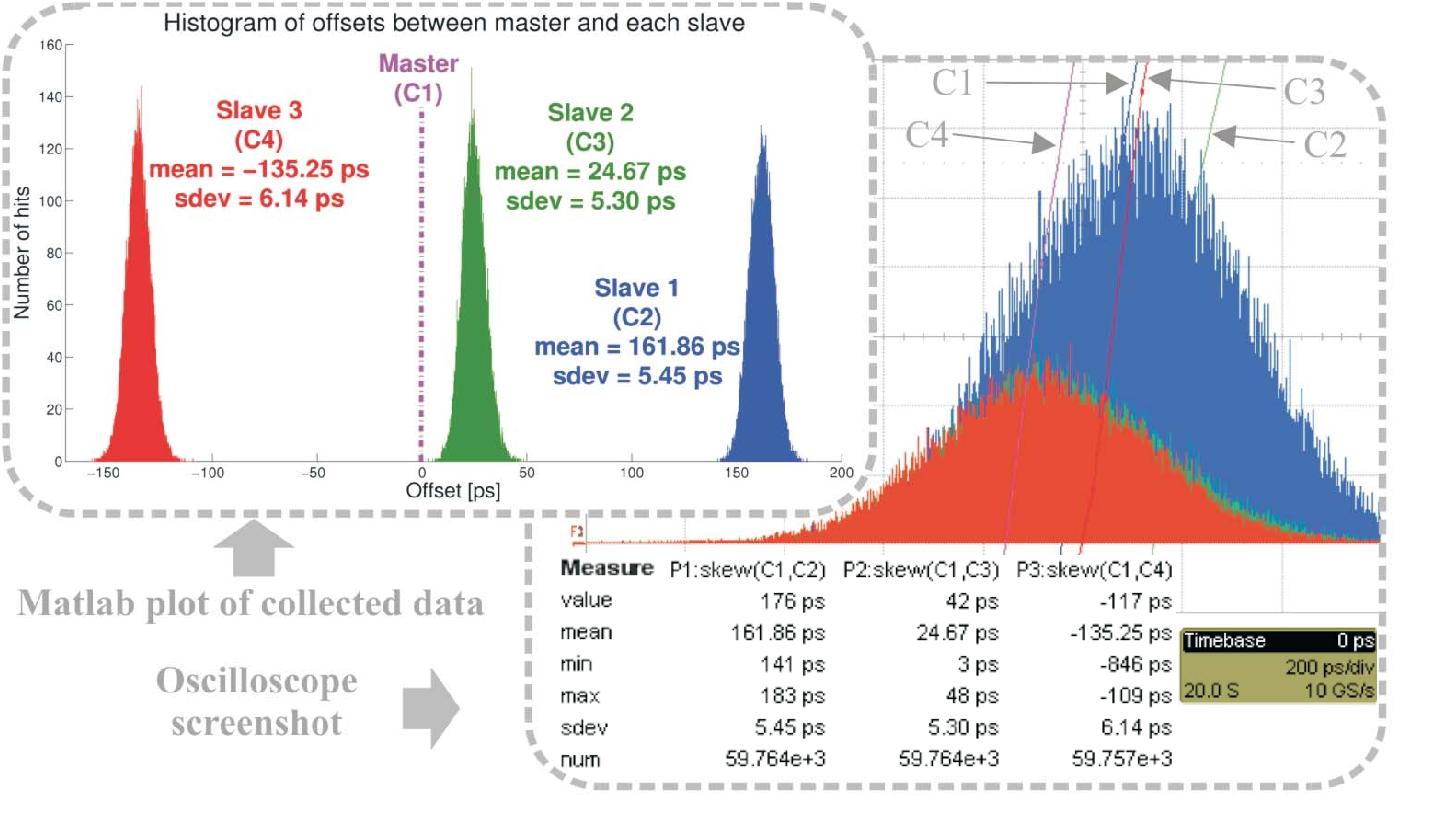
\includegraphics[height=6.0cm]{measurements/measResults-new.pdf}
    \end{center}


\end{frame}
%%%%%%%%%%%%%%%%%%%%%%%%%%%%%%%%%%%%%%%%%%%%%%%%%%%%%%%%%%%%%%%%%%%%%%%%%%%%%%%%%%%%%%%%%%%%%%%%%%%%
%\section{Status}
%\subsection{}
%%%%%%%%%%%%%%%%%%%%%%%%%%%%%%%%%%%%%%%%%%%%%%%%%%%%%%%%%%%%%%%%%%%%%%%%%%%%%%%%%%%%%%%%%%%%%%%%%%%%
\begin{frame}{Testy: wpływ temperatury na synchronizację}

    \begin{center}
    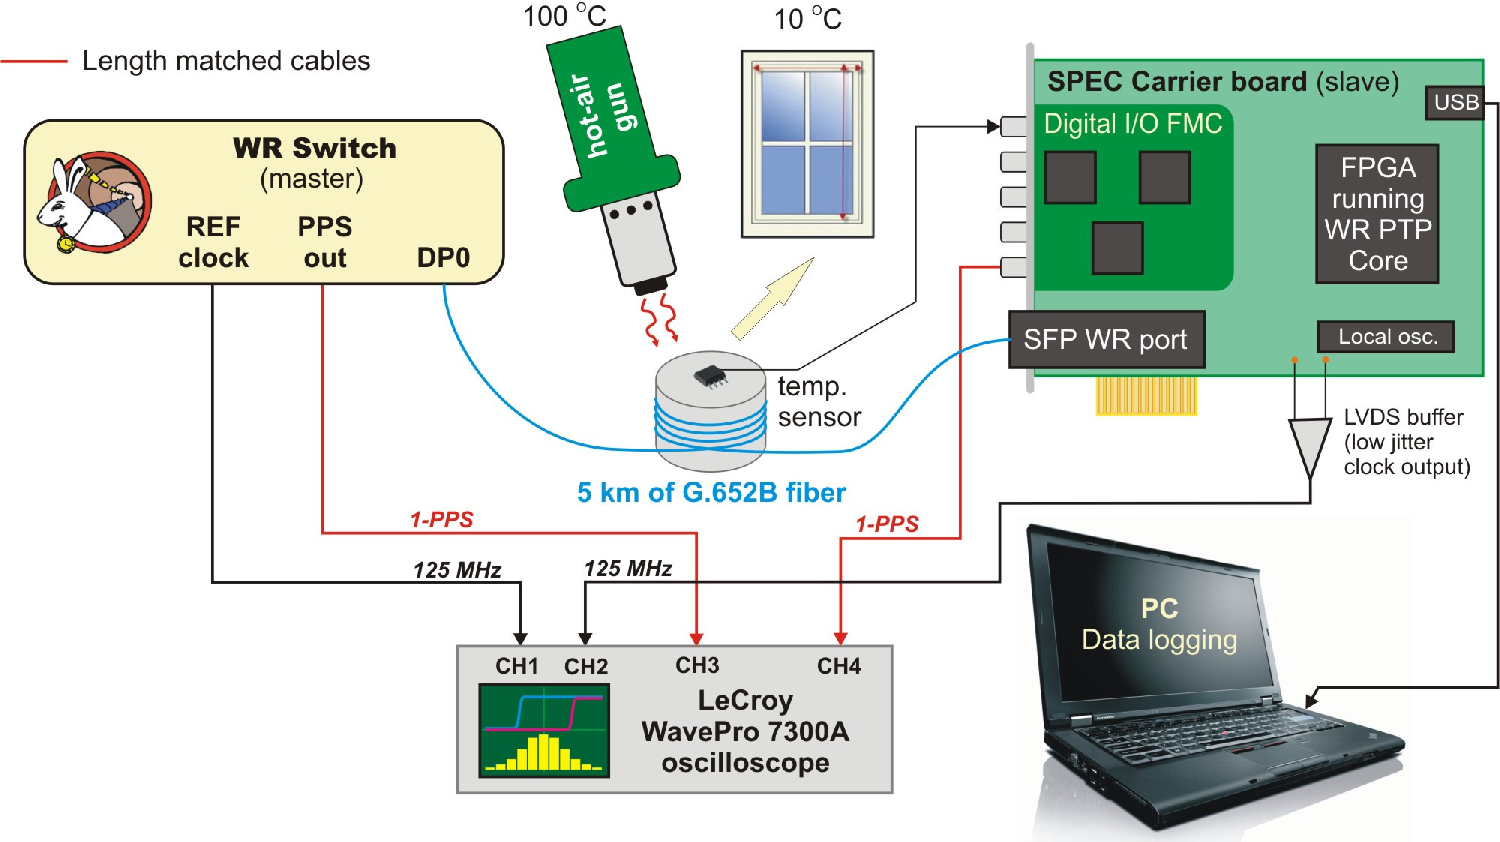
\includegraphics[height=6.0cm]{measurements/meas_system_wrcore.pdf}
    \end{center}

\end{frame}
%%%%%%%%%%%%%%%%%%%%%%%%%%%%%%%%%%%%%%%%%%%%%%%%%%%%%%%%%%%%%%%%%%%%%%%%%%%%%%%%%%%%%%%%%%%%%%%%%%%%
% \subsection{}
%%%%%%%%%%%%%%%%%%%%%%%%%%%%%%%%%%%%%%%%%%%%%%%%%%%%%%%%%%%%%%%%%%%%%%%%%%%%%%%%%%%%%%%%%%%%%%%%%%%%
\begin{frame}{Testy : Delay vs. temperature}

  \begin{center}
  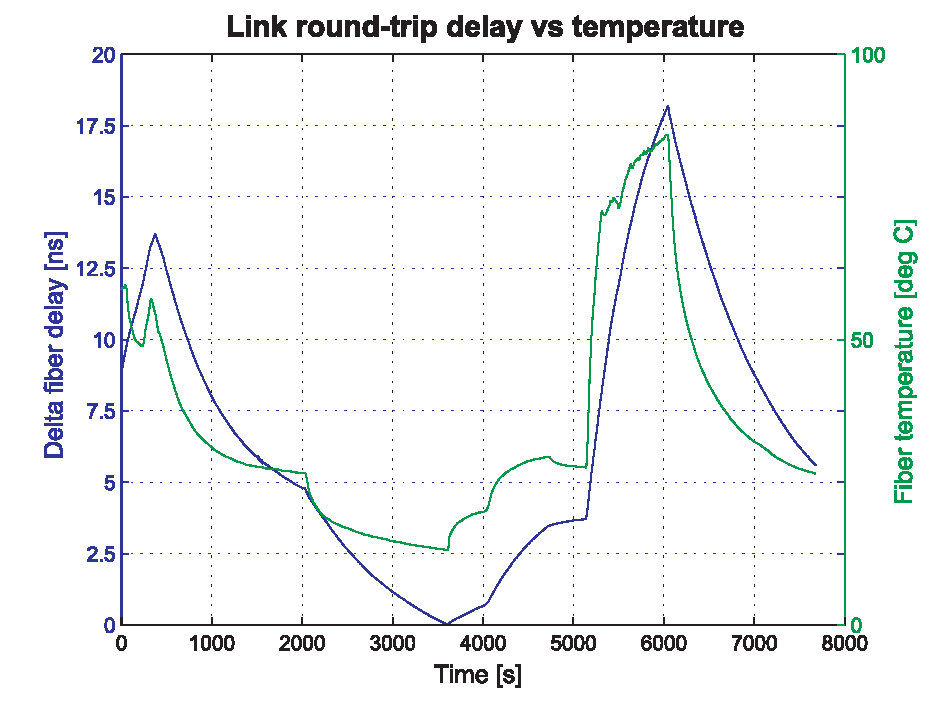
\includegraphics[width=7cm]{measurements/wrpc_delay_vs_temp.pdf}

  Zakres temperatury: 80 degC
  \end{center}

\end{frame}
%%%%%%%%%%%%%%%%%%%%%%%%%%%%%%%%%%%%%%%%%%%%%%%%%%%%%%%%%%%%%%%%%%%%%%%%%%%%%%%%%%%%%%%%%%%%%%%%%%%%
% \subsection{}
%%%%%%%%%%%%%%%%%%%%%%%%%%%%%%%%%%%%%%%%%%%%%%%%%%%%%%%%%%%%%%%%%%%%%%%%%%%%%%%%%%%%%%%%%%%%%%%%%%%%
\begin{frame}{Testy: Offset vs. temperature}

  \begin{center}
    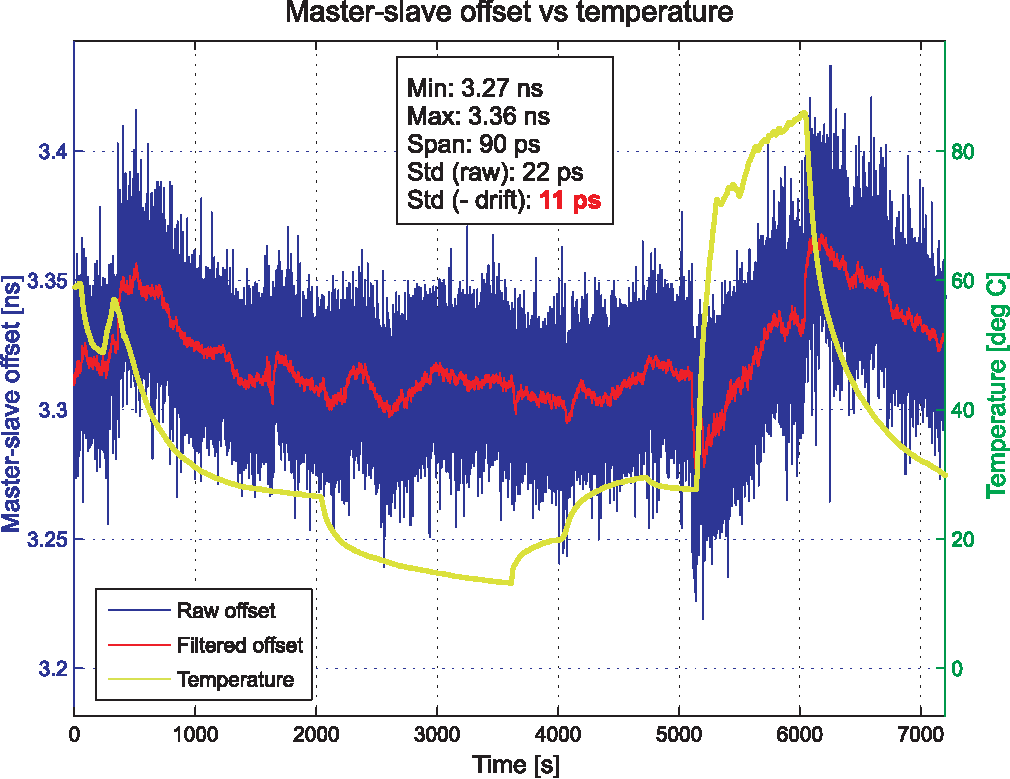
\includegraphics[width=7cm]{measurements/wrpc_offset_vs_temp.pdf}
  \end{center}
  \begin{itemize}
%    \item Measured on reference clocks (125 MHz) bypassing the FPGA.
    \item Dryft offsetu w zakresie temperatury 80 deg C: \textbf{90 ps}
    \item 22 ps rms jitter, 12 ps gdy odejmiemy dryft offsetu
  \end{itemize}

\end{frame}

%%%%%%%%%%% part 2



%%%%%%%%%%%%%%%%%%%%%%%%%%%%%%%%%%%%%%%%%%%%%%%%%%%%%%%%%%%%%%%%%%%%%%%%%%%%%%%%%%%%%%%%%%%%%%%%%%%%
\section{Dystrybucja danych w sieci WR}
\subsection{}
%%%%%%%%%%%%%%%%%%%%%%%%%%%%%%%%%%%%%%%%%%%%%%%%%%%%%%%%%%%%%%%%%%%%%%%%%%%%%%%%%%%%%%%%%%%%%%%%%%%%
\begin{frame}{Dystrybucja danych w sieci White Rabbit}

  \begin{center}
     \color{red}{Deterministyczny i niezawodny transfer danych}
  \end{center}

\end{frame}




%%%%%%%%%%%%%%%%%%%%%%%%%%%%%%%%%%%%%%%%%%%%%%%%%%%%%%%%%%%%%%%%%%%%%%%%%%%%%%%%%%%%%%%%%%%%%%%%%%%%
% \subsection{}
%%%%%%%%%%%%%%%%%%%%%%%%%%%%%%%%%%%%%%%%%%%%%%%%%%%%%%%%%%%%%%%%%%%%%%%%%%%%%%%%%%%%%%%%%%%%%%%%%%%%
\begin{frame}{Dystrybucja danych kontrolnych}

    \begin{center}
    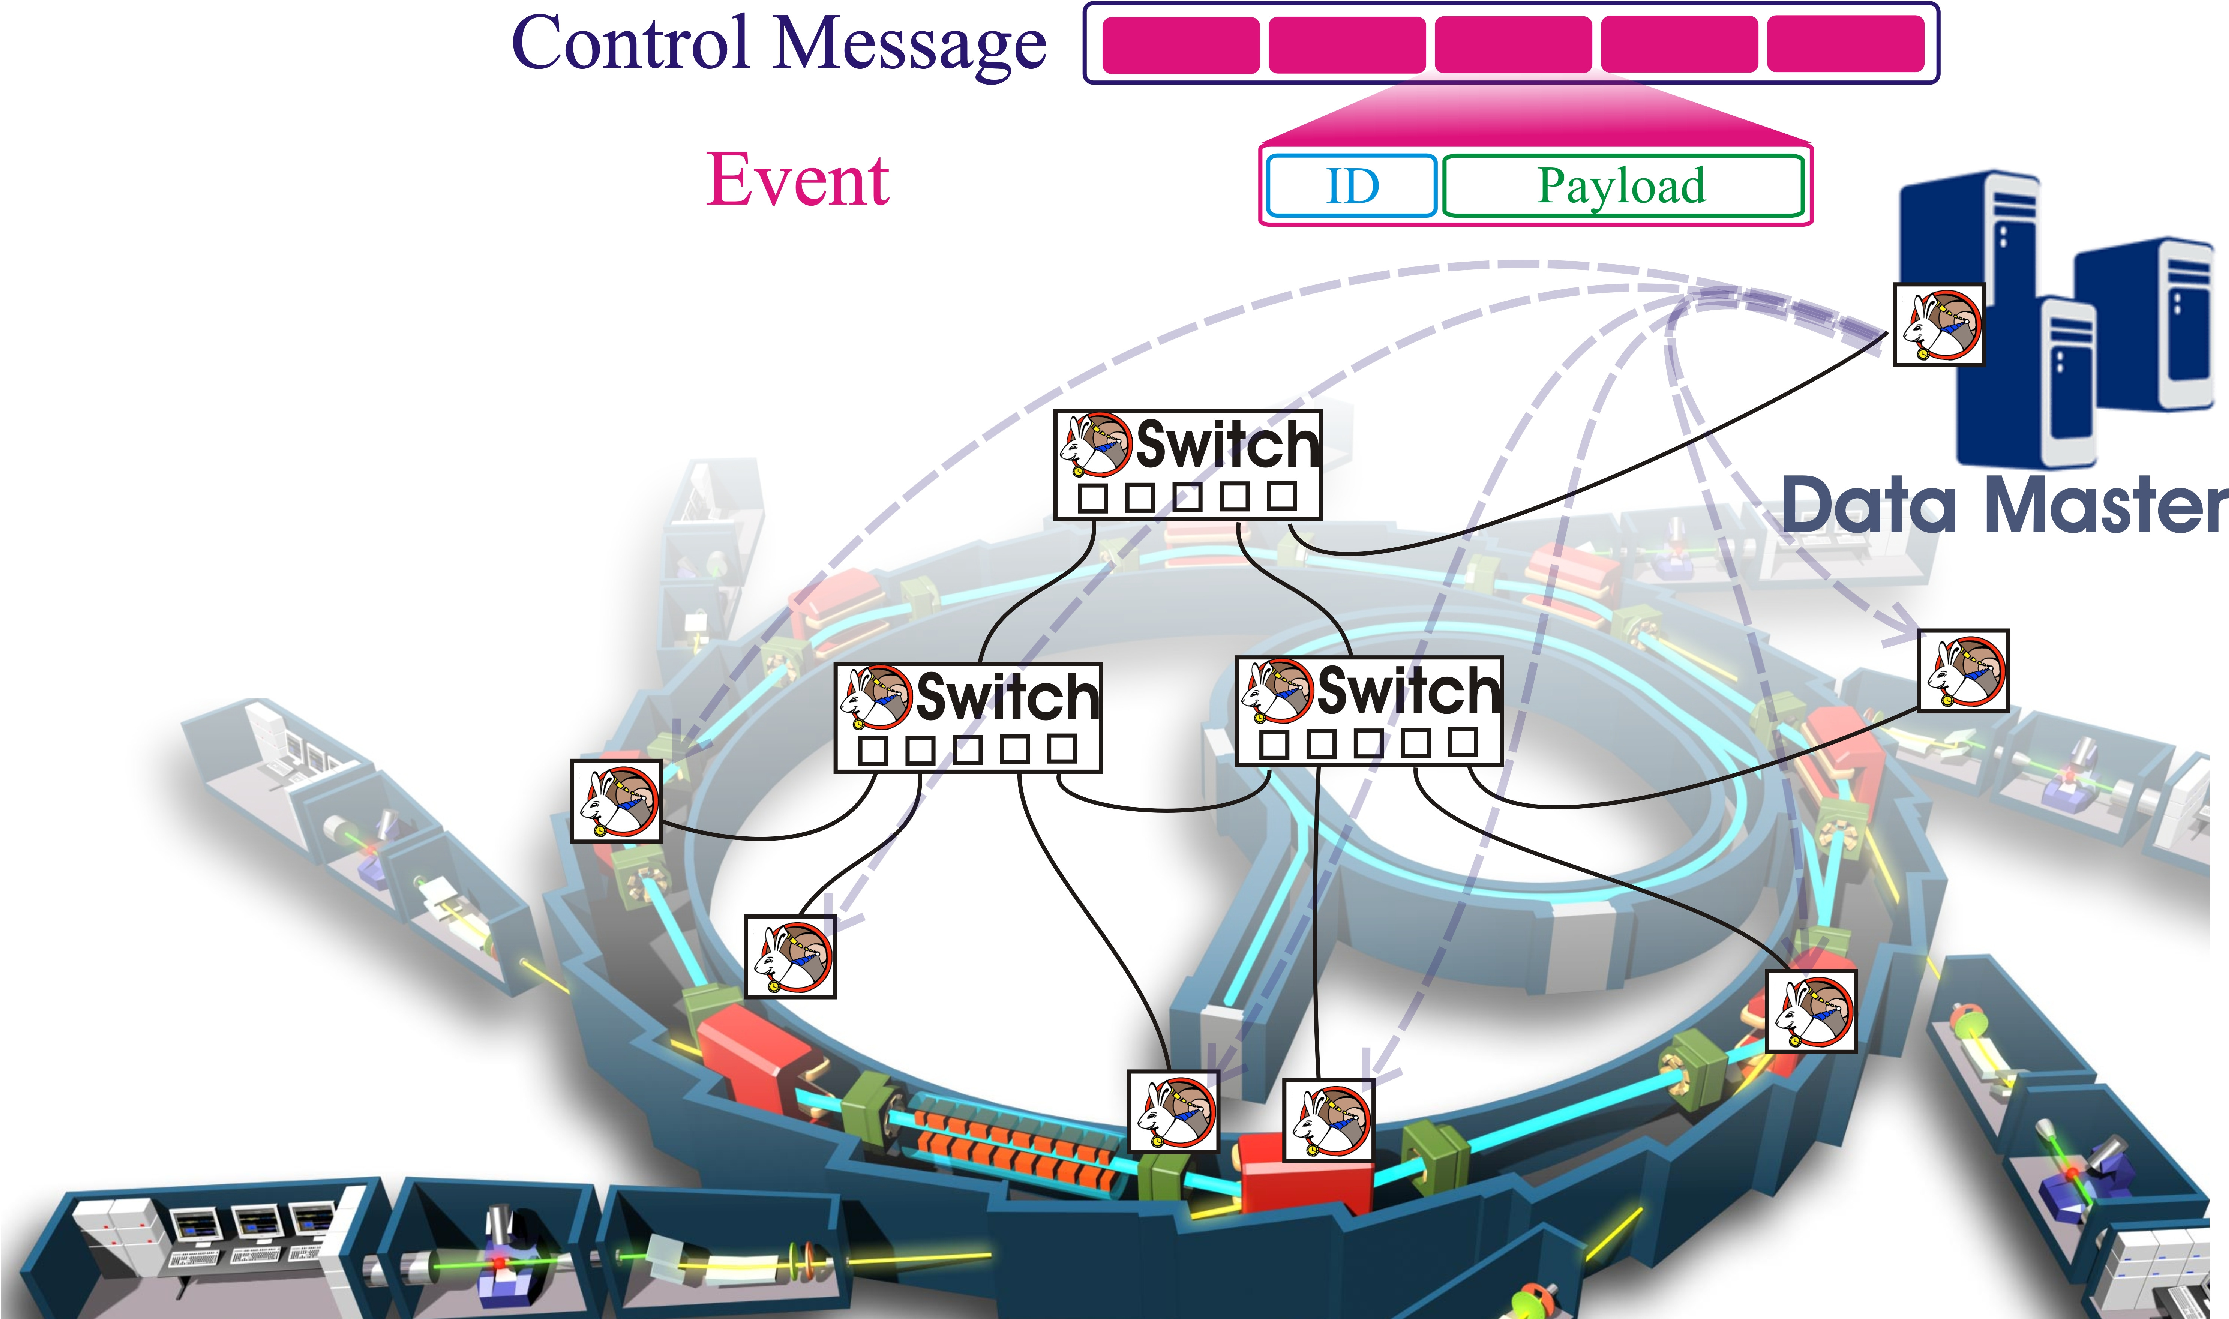
\includegraphics[width=1.1\textwidth]{applications/CERN/WRControlNetwork.pdf}
    \end{center}


\end{frame}
%%%%%%%%%%%%%%%%%%%%%%%%%%%%%%%%%%%%%%%%%%%%%%%%%%%%%%%%%%%%%%%%%%%%%%%%%%%%%%%%%%%%%%%%%%%%%%%%%%%%
% \subsection{}
%%%%%%%%%%%%%%%%%%%%%%%%%%%%%%%%%%%%%%%%%%%%%%%%%%%%%%%%%%%%%%%%%%%%%%%%%%%%%%%%%%%%%%%%%%%%%%%%%%%%
\begin{frame}{Wymagania dot. dystrybucji danych w CERN i GSI}

    \begin{center}
    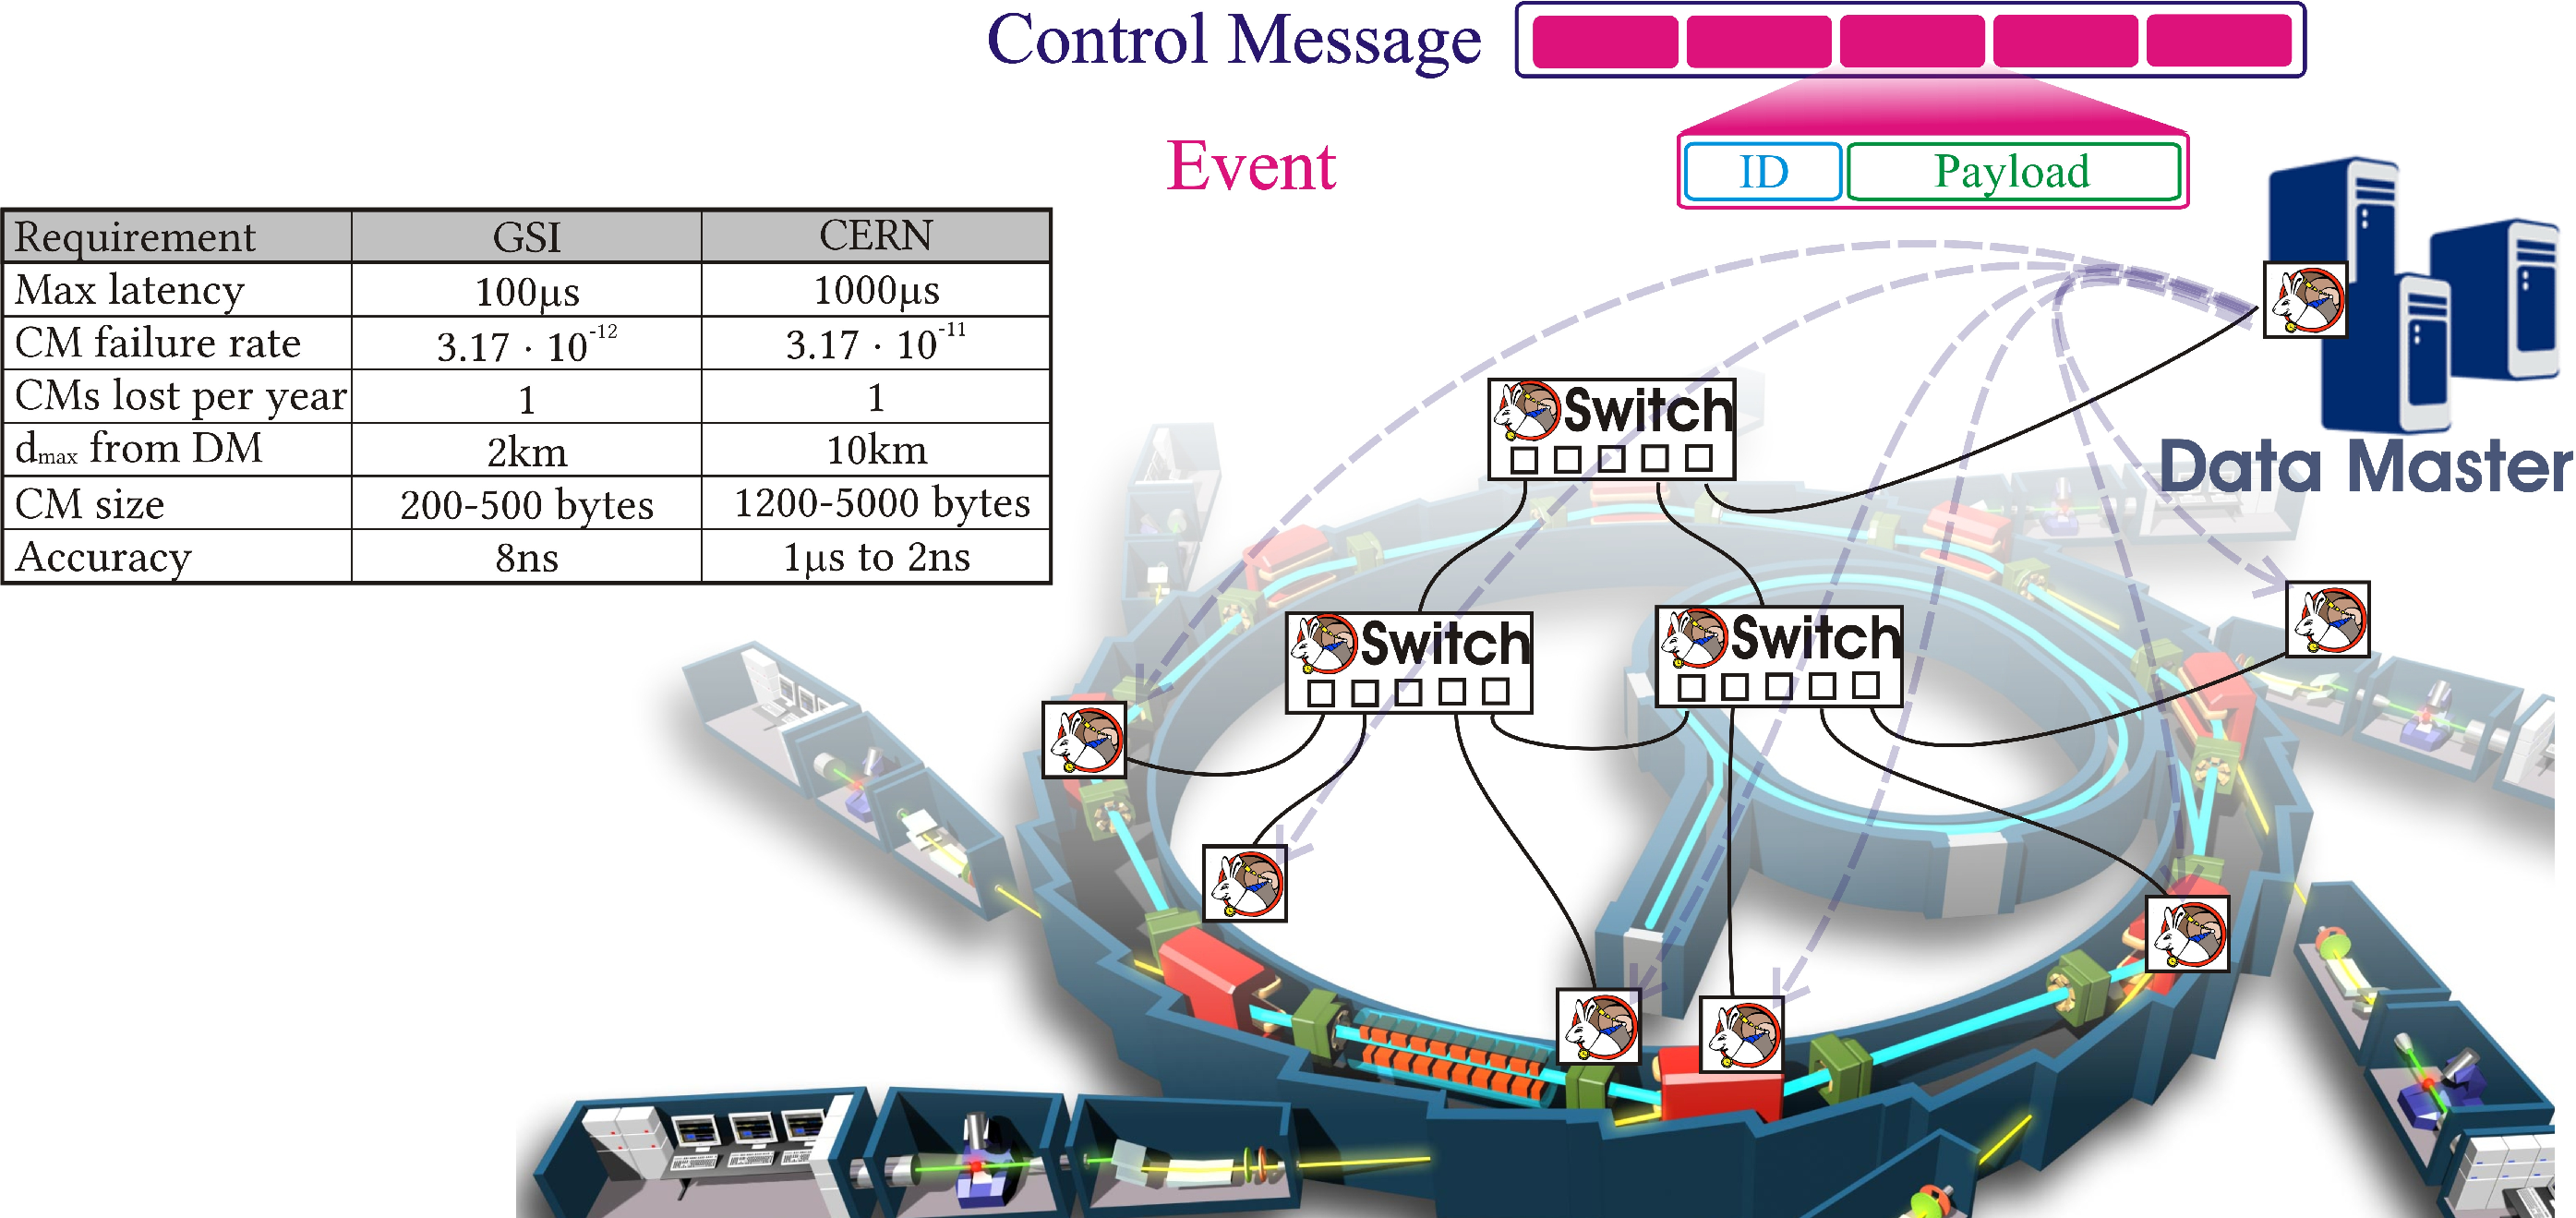
\includegraphics[width=1.1\textwidth]{applications/CERN/WRControlNetwork2.pdf}
    \end{center}


\end{frame}
%%%%%%%%%%%%%%%%%%%%%%%%%%%%%%%%%%%%%%%%%%%%%%%%%%%%%%%%%%%%%%%%%%%%%%%%%%%%%%%%%%%%%%%%%%%%%%%%%%%%
% \subsection{}
%%%%%%%%%%%%%%%%%%%%%%%%%%%%%%%%%%%%%%%%%%%%%%%%%%%%%%%%%%%%%%%%%%%%%%%%%%%%%%%%%%%%%%%%%%%%%%%%%%%%
\begin{frame}{Poprawne działanie systemu}


  System działa poprawnie kiedy spełnione są następujące warunki :
  
  \begin{itemize}
    \item \color{blue}{Wszystkie odbiorniki (nodes) są z synchronizowane z wymaganą dokładnością}
    \item  \color{red}{Wszystkie odbiorniki (nodes) otrzymują dane kontrolne (Control Messages)}
    \item  \color{red}{Dane kontrolne (Control Messages) docierają do wszystkich odbiorników (nodes)
          w czasie mniejszym niż wymagana maksymalna latencja.}
  \end{itemize}

\end{frame}
%%%%%%%%%%%%%%%%%%%%%%%%%%%%%%%%%%%%%%%%%%%%%%%%%%%%%%%%%%%%%%%%%%%%%%%%%%%%%%%%%%%%%%%%%%%%%%%%%%%%
% \subsection{}
%%%%%%%%%%%%%%%%%%%%%%%%%%%%%%%%%%%%%%%%%%%%%%%%%%%%%%%%%%%%%%%%%%%%%%%%%%%%%%%%%%%%%%%%%%%%%%%%%%%%
\begin{frame}{Identyfikacja powodów awarii systemu}


  \begin{itemize}
    \item Przekłamanie danych (bit errors)
    \item Przeciążenie sieci (congestion)
    \item Awaria elementów sieci (element failure)
    \item Zbyt długi czas transmisji (exceeding upper bound latency)
  \end{itemize}

\end{frame}

%%%%%%%%%%%%%%%%%%%%%%%%%%%%%%%%%%%%%%%%%%%%%%%%%%%%%%%%%%%%%%%%%%%%%%%%%%%%%%%%%%%%%%%%%%%%%%%%%%%%
% \subsection{}
%%%%%%%%%%%%%%%%%%%%%%%%%%%%%%%%%%%%%%%%%%%%%%%%%%%%%%%%%%%%%%%%%%%%%%%%%%%%%%%%%%%%%%%%%%%%%%%%%%%%
\begin{frame}{Identyfikacja powodów awarii systemu}


  \begin{itemize}
    \item \color{red}{Przekłamanie danych (bit errors)}
    \item \color{black}{Przeciążenie sieci (congestion)}
    \item Awaria elementów sieci (element failure)
    \item Zbyt długi czas transmisji (exceeding upper bound latency)
  \end{itemize}

\end{frame}

%%%%%%%%%%%%%%%%%%%%%%%%%%%%%%%%%%%%%%%%%%%%%%%%%%%%%%%%%%%%%%%%%%%%%%%%%%%%%%%%%%%%%%%%%%%%%%%%%%%%
% \subsection{}
%%%%%%%%%%%%%%%%%%%%%%%%%%%%%%%%%%%%%%%%%%%%%%%%%%%%%%%%%%%%%%%%%%%%%%%%%%%%%%%%%%%%%%%%%%%%%%%%%%%%
\begin{frame}{Niezawodny przesył danych}

  \begin{columns}[c]
  \column{.6\textwidth} 

      \begin{itemize}
	\item Retransmisja danych niemożliwa
	\item Kanał komunikacyjny, dwa modele:
	\begin{itemize}
	  \item Binary erasure channel (BEC)
	  \item Packet erasure channel (PEC)
	\end{itemize}
	\item Bit error rate (BER) - prawdopodobieństwo przekłamania bitu informacji w strumieniu danych, 
	      różne dla różnych nośników
	\item Forward Error Correction (FEC) - kodowanie nadmiarowe
      \end{itemize}

      \vspace{2cm}

  \column{.4\textwidth} 

      \begin{center}
      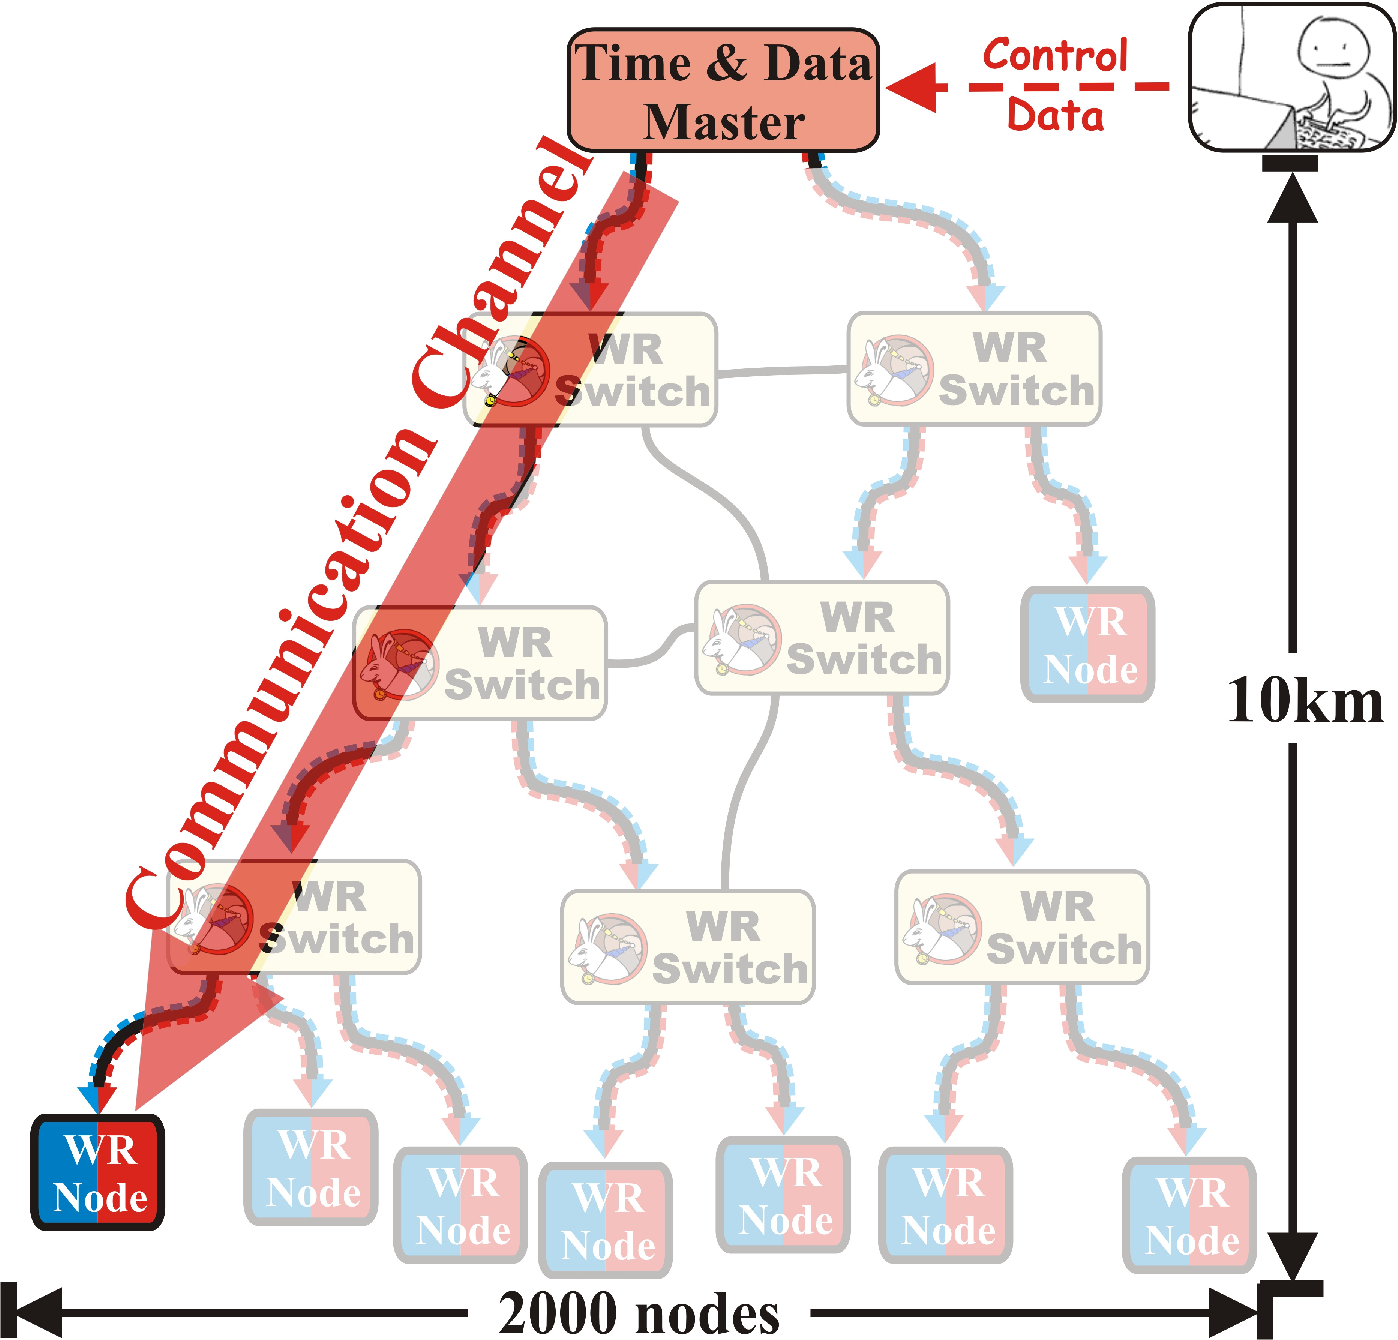
\includegraphics[width=4.5cm]{robustness/CommunicationChannel.pdf}
      \end{center}

      \vspace{2cm}

  \end{columns}

\end{frame}
%%%%%%%%%%%%%%%%%%%%%%%%%%%%%%%%%%%%%%%%%%%%%%%%%%%%%%%%%%%%%%%%%%%%%%%%%%%%%%%%%%%%%%%%%%%%%%%%%%%%
% \subsection{}
%%%%%%%%%%%%%%%%%%%%%%%%%%%%%%%%%%%%%%%%%%%%%%%%%%%%%%%%%%%%%%%%%%%%%%%%%%%%%%%%%%%%%%%%%%%%%%%%%%%%
\begin{frame}{Forward Error Correction}

      \begin{itemize}
	\item Packet erasure channel (PEC) -- {\bf Reed-Solomon}
	\begin{itemize}
	  \item Tworzymy 4 pakiety z oryginalnej wiadomości
	  \item Otrzymanie 2 z 4 pakietów pozwala na odtworzenie wiadomości
	\end{itemize}
	\item Binary erasure channel (BEC) -- {\bf Hamming} with additional Parity
	\begin{itemize}
	  \item Hamming distance = 4
	  \item Korekcja pojedynczego przekłamania bitu i detekcja podwójnego przekłamania
	\end{itemize}    
      \end{itemize}


      \begin{center}
      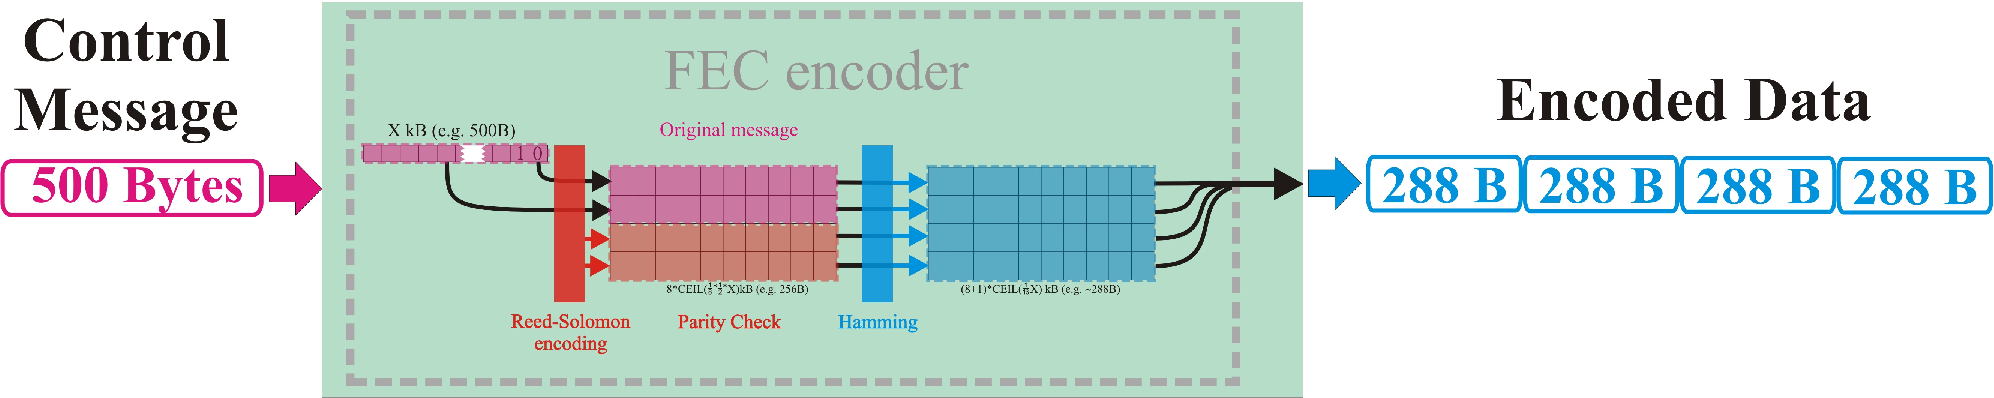
\includegraphics[width=1.0\textwidth]{robustness/FECencoder.pdf}
      \end{center}

\end{frame}
%%%%%%%%%%%%%%%%%%%%%%%%%%%%%%%%%%%%%%%%%%%%%%%%%%%%%%%%%%%%%%%%%%%%%%%%%%%%%%%%%%%%%%%%%%%%%%%%%%%%
% \subsection{}
%%%%%%%%%%%%%%%%%%%%%%%%%%%%%%%%%%%%%%%%%%%%%%%%%%%%%%%%%%%%%%%%%%%%%%%%%%%%%%%%%%%%%%%%%%%%%%%%%%%%
\begin{frame}{Identyfikacja powodów awarii systemu}


  \begin{itemize}
    \item Przekłamanie danych (bit errors)
    \item  \color{red}{{\bf Przeciążenie sieci (congestion)}}
    \item \color{black}{Awaria elementów sieci (element failure)}
    \item Zbyt długi czas transmisji (exceeding upper bound latency)
  \end{itemize}

\end{frame}
%%%%%%%%%%%%%%%%%%%%%%%%%%%%%%%%%%%%%%%%%%%%%%%%%%%%%%%%%%%%%%%%%%%%%%%%%%%%%%%%%%%%%%%%%%%%%%%%%%%%
% \subsection{}
%%%%%%%%%%%%%%%%%%%%%%%%%%%%%%%%%%%%%%%%%%%%%%%%%%%%%%%%%%%%%%%%%%%%%%%%%%%%%%%%%%%%%%%%%%%%%%%%%%%%
\begin{frame}{Quality of service}


  \begin{itemize}
    \item Wykorzystujemy priorytetyzację przesyłanych danych (IEEE 802.1Q)
    \item Najwyższy priorytet dla Control Messages
    \item Implementacja switcha zapewnia odpowiednie zasoby
  \end{itemize}

\end{frame}

%%%%%%%%%%%%%%%%%%%%%%%%%%%%%%%%%%%%%%%%%%%%%%%%%%%%%%%%%%%%%%%%%%%%%%%%%%%%%%%%%%%%%%%%%%%%%%%%%%%%
% \subsection{}
%%%%%%%%%%%%%%%%%%%%%%%%%%%%%%%%%%%%%%%%%%%%%%%%%%%%%%%%%%%%%%%%%%%%%%%%%%%%%%%%%%%%%%%%%%%%%%%%%%%%
\begin{frame}{Identyfikacja powodów awarii systemu}


  \begin{itemize}
    \item Przekłamanie danych (bit errors)
    \item Przeciążenie sieci (congestion)
    \item \color{red}{{\bf Awaria elementów sieci (element failure)}}
    \item \color{black}{Zbyt długi czas transmisji (exceeding upper bound latency)}
  \end{itemize}

\end{frame}
%%%%%%%%%%%%%%%%%%%%%%%%%%%%%%%%%%%%%%%%%%%%%%%%%%%%%%%%%%%%%%%%%%%%%%%%%%%%%%%%%%%%%%%%%%%%%%%%%%%%
% \subsection{}
%%%%%%%%%%%%%%%%%%%%%%%%%%%%%%%%%%%%%%%%%%%%%%%%%%%%%%%%%%%%%%%%%%%%%%%%%%%%%%%%%%%%%%%%%%%%%%%%%%%%
\begin{frame}{Niezawodność sieci}


  \begin{columns}[c]
  \column{.5\textwidth} 

  \begin{itemize}
    \item Pomiar niezawodności: Mean Time Between Failures (MTBF)
    \item Zwiększenie niezawodności:
    \begin{itemize}
      \item wprowadzenie elementów nadmiarowych
      \item eliminacja Single Point of Failure (SPoF)
    \end{itemize}
    \item Nadmiarowe topologia sieci
  \end{itemize}

      \vspace{2cm}

  \column{.5\textwidth} 

      \begin{center}
      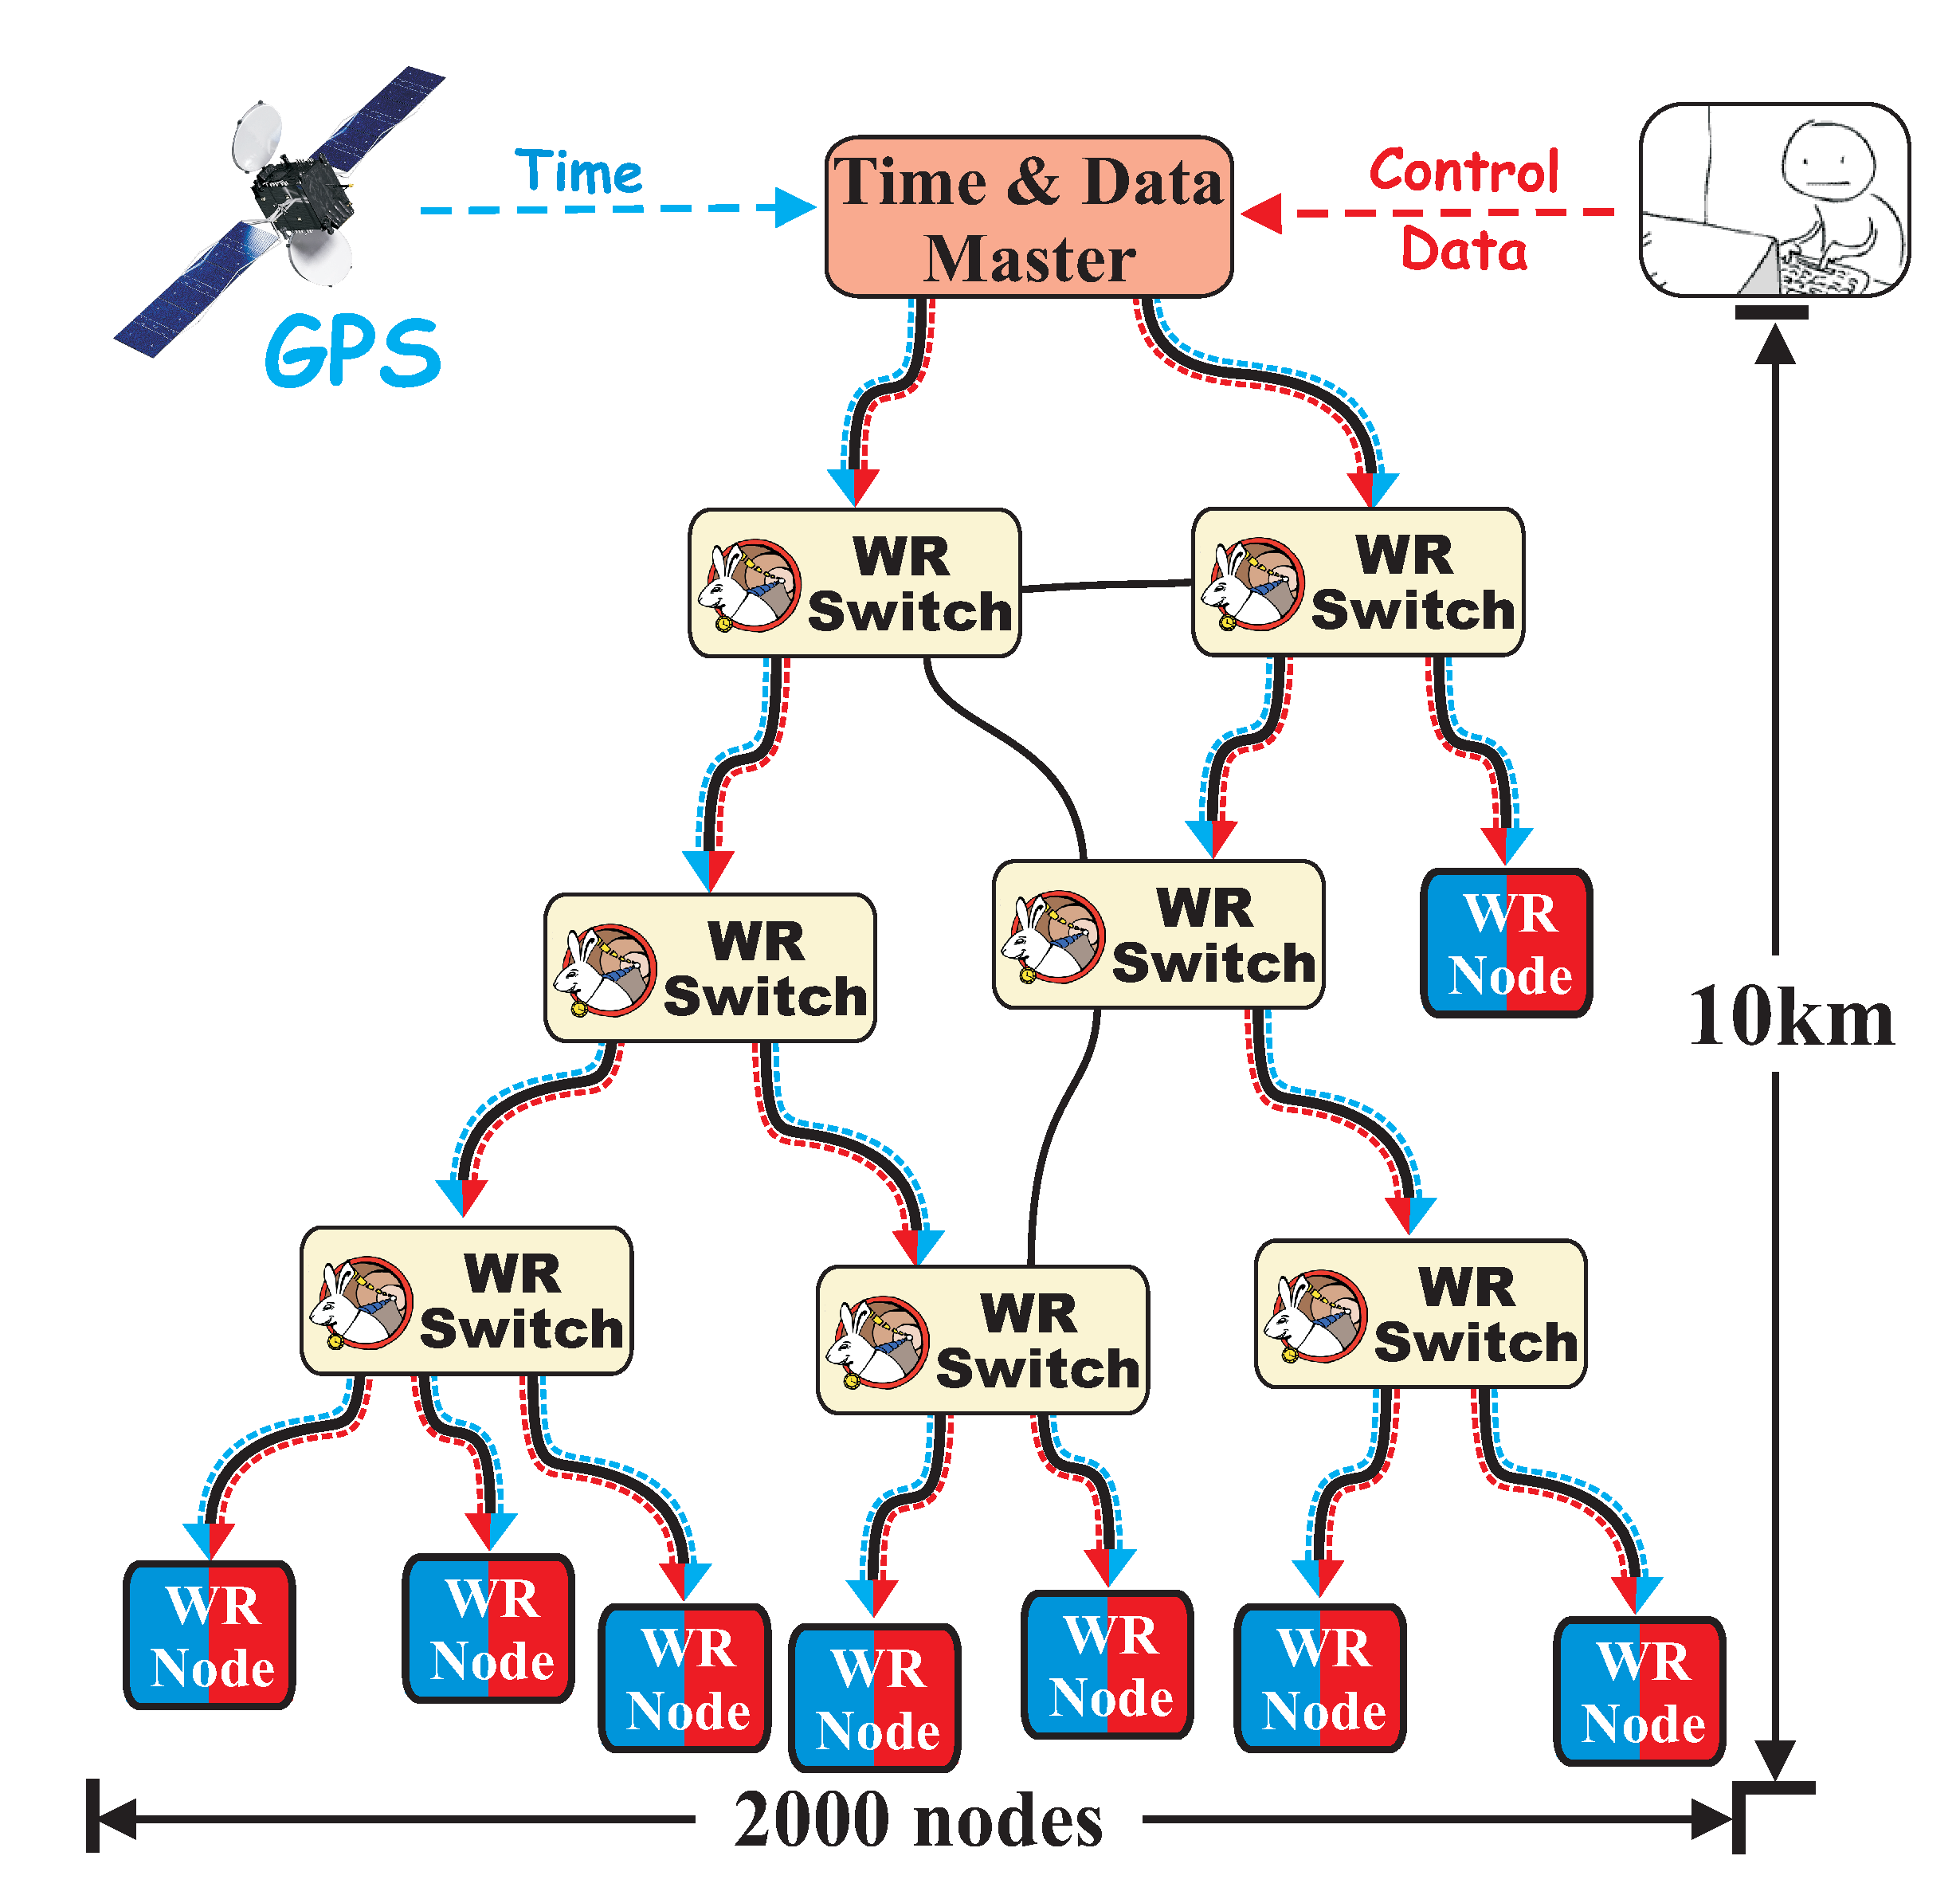
\includegraphics[width=6cm]{network/wr_network-new.pdf}
      \end{center}

      \vspace{2cm}

  \end{columns}

\end{frame}
%%%%%%%%%%%%%%%%%%%%%%%%%%%%%%%%%%%%%%%%%%%%%%%%%%%%%%%%%%%%%%%%%%%%%%%%%%%%%%%%%%%%%%%%%%%%%%%%%%%%
% \subsection{}
%%%%%%%%%%%%%%%%%%%%%%%%%%%%%%%%%%%%%%%%%%%%%%%%%%%%%%%%%%%%%%%%%%%%%%%%%%%%%%%%%%%%%%%%%%%%%%%%%%%%
\begin{frame}{FEC + Nadmiarowość sieci}

  \begin{itemize}
    \item Bardzo szybka detekcja awarii i przełączenie miedzy nadmiarowymi połączeniami
    \item Maksymalny czas trwania procesu: czas transmisji ramki: $\approx 2.3 \mu$
    \item Najlepsze parametry znanych rozwiązań: milisekundy
  \end{itemize}

      \begin{center}
      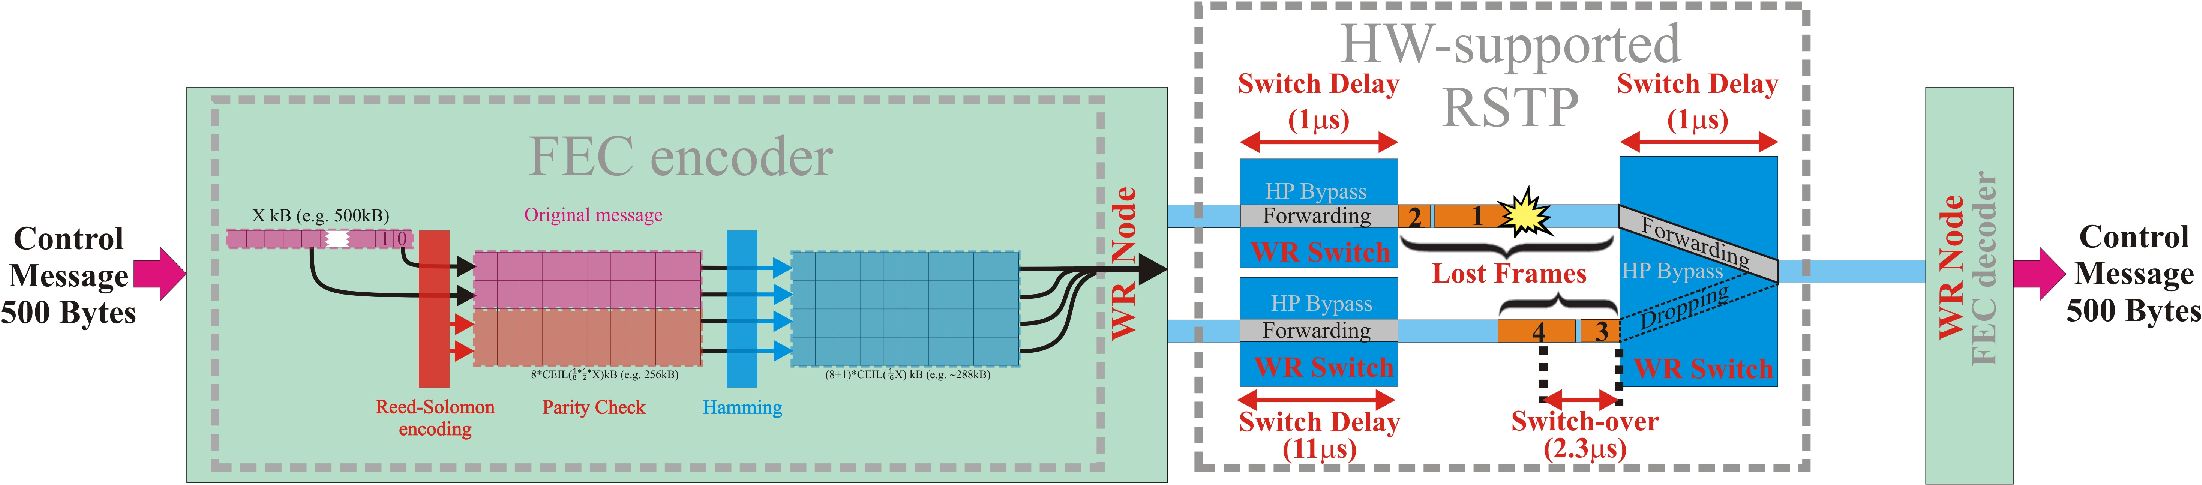
\includegraphics[width=1.0\textwidth]{robustness/FECandRSTP.pdf}
      \end{center}


\end{frame}
%%%%%%%%%%%%%%%%%%%%%%%%%%%%%%%%%%%%%%%%%%%%%%%%%%%%%%%%%%%%%%%%%%%%%%%%%%%%%%%%%%%%%%%%%%%%%%%%%%%%
% \subsection{}
%%%%%%%%%%%%%%%%%%%%%%%%%%%%%%%%%%%%%%%%%%%%%%%%%%%%%%%%%%%%%%%%%%%%%%%%%%%%%%%%%%%%%%%%%%%%%%%%%%%%
\begin{frame}{Identyfikacja powodów awarii systemu}


  \begin{itemize}
    \item Przekłamanie danych (bit errors)
    \item Przeciążenie sieci (congestion)
    \item Awaria elementów sieci (element failure)
    \item \color{red}{{\bf Zbyt długi czas transmisji (exceeding upper bound latency)}}
  \end{itemize}

\end{frame}


%%%%%%%%%%%%%%%%%%%%%%%%%%%%%%%%%%%%%%%%%%%%%%%%%%%%%%%%%%%%%%%%%%%%%%%%%%%%%%%%%%%%%%%%%%%%%%%%%%%%
% \subsection{}
%%%%%%%%%%%%%%%%%%%%%%%%%%%%%%%%%%%%%%%%%%%%%%%%%%%%%%%%%%%%%%%%%%%%%%%%%%%%%%%%%%%%%%%%%%%%%%%%%%%%
\begin{frame}{Determinizm transmisji danych}


  \begin{columns}[c]
  \column{.5\textwidth} 

  

  \begin{itemize}
    \item Bardzo rozważna architektura topologi sieci
    \item Oszacowanie maksymalnego opóźnienia dla najdłuższej ścieżki
    \item Oszacowany czas transmisji niekorzystny dla GSI
    \item Zmiana architektury switcha
  \end{itemize}

  
  \column{.5\textwidth} 

      \begin{center}
      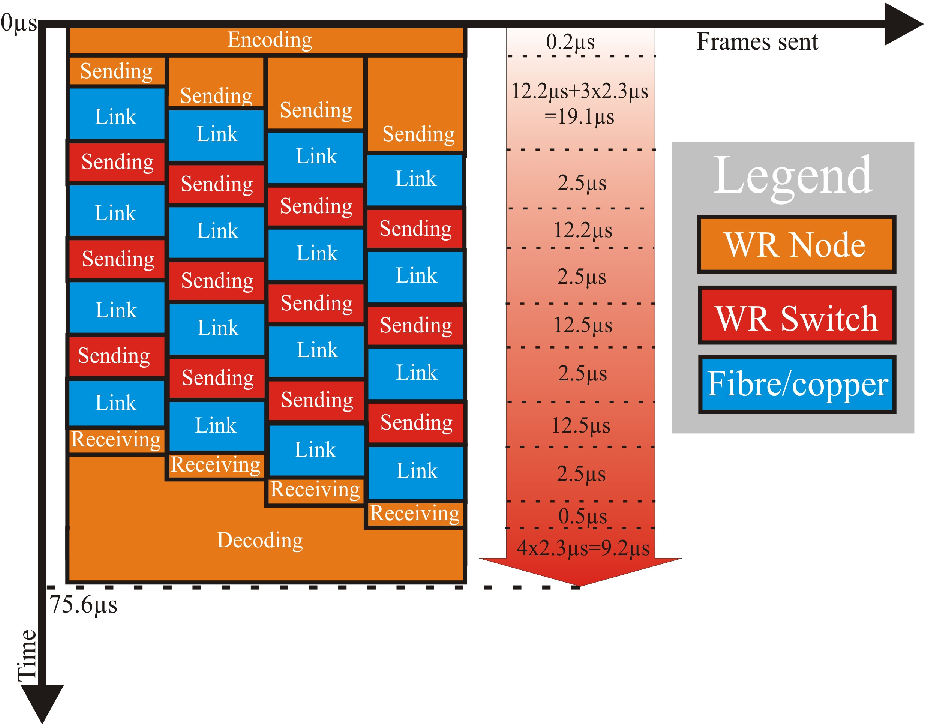
\includegraphics[width=6cm]{robustness/latencyEstimation.pdf}
      \end{center}

      

  \end{columns}


\end{frame}


%%%%%%%%%%%%%%%%%%%%%%%%%%%%%%%%%%%%%%%%%%%%%%%%%%%%%%%%%%%%%%%%%%%%%%%%%%%%%%%%%%%%%%%%%%%%%%%%%%%%
\section{Elementy sieci WR}
\subsection{}
%%%%%%%%%%%%%%%%%%%%%%%%%%%%%%%%%%%%%%%%%%%%%%%%%%%%%%%%%%%%%%%%%%%%%%%%%%%%%%%%%%%%%%%%%%%%%%%%%%%%
\begin{frame}{Elementy systemu White Rabbit}

      \begin{center}
      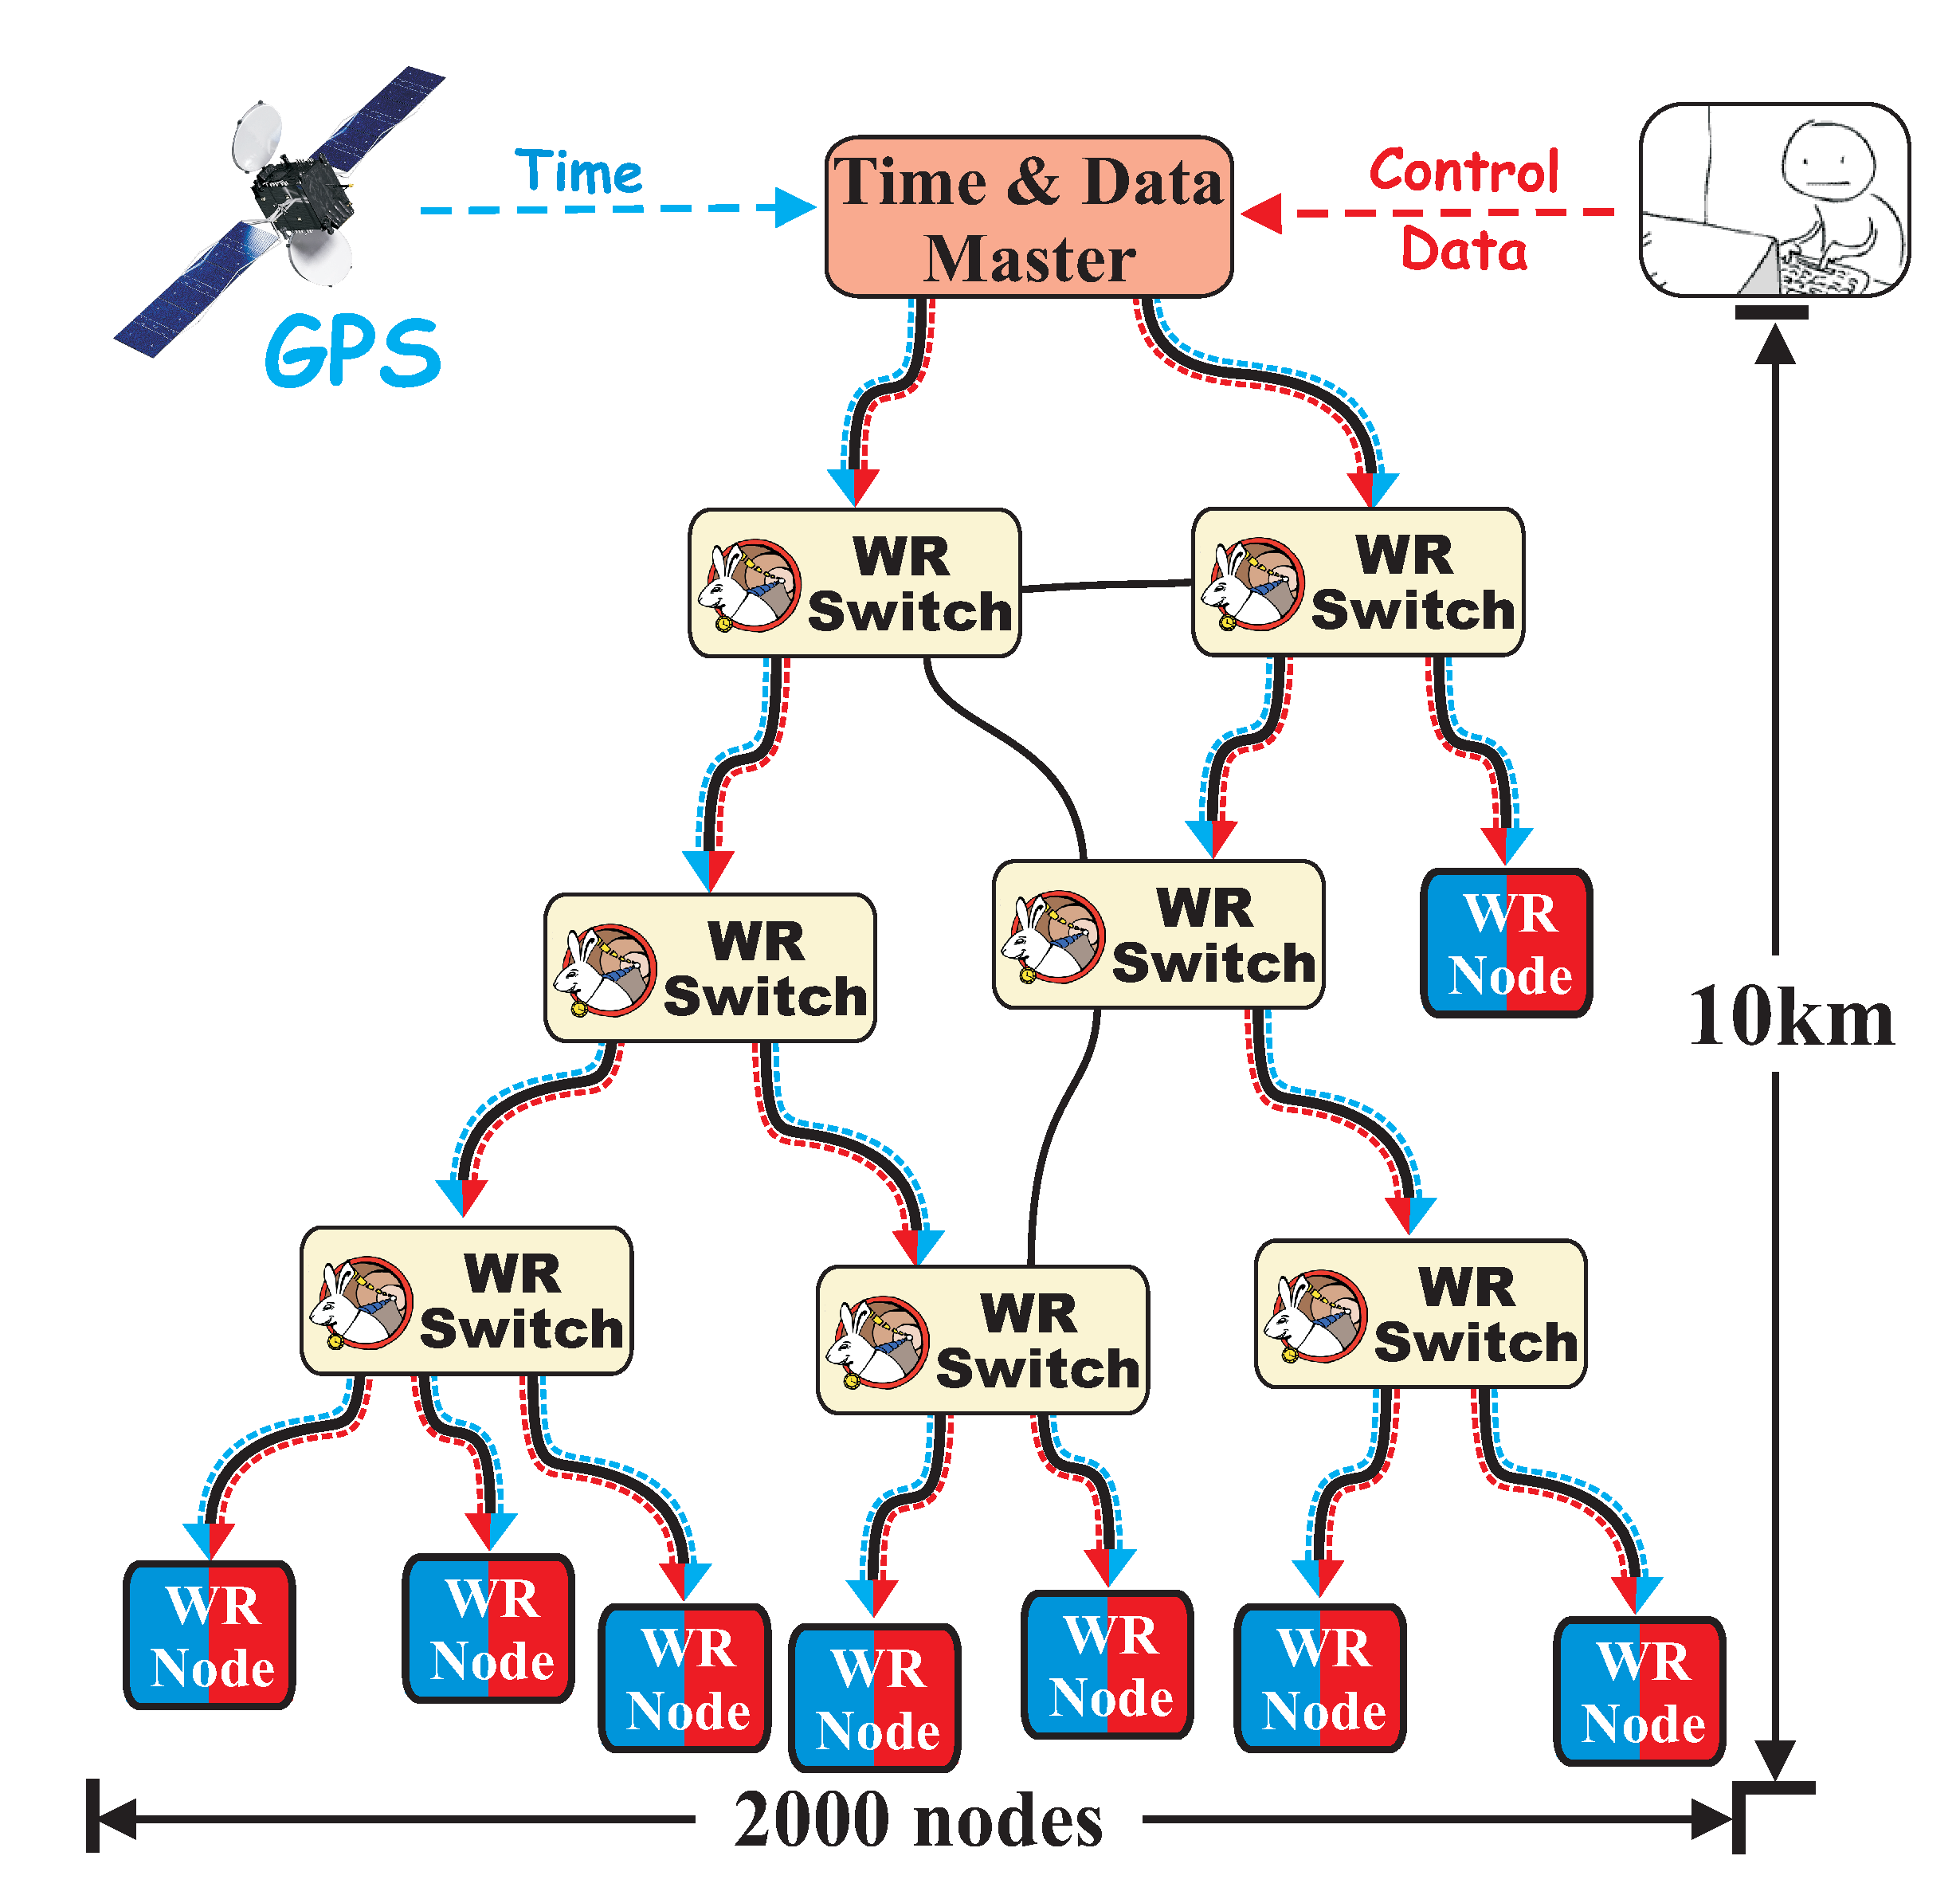
\includegraphics[width=7cm]{network/wr_network-new.pdf}
      \end{center}

\end{frame}

%%%%%%%%%%%%%%%%%%%%%%%%%%%%%%%%%%%%%%%%%%%%%%%%%%%%%%%%%%%%%%%%%%%%%%%%%%%%%%%%%%%%%%%%%%%%%%%%%%%%
% \subsection{}
%%%%%%%%%%%%%%%%%%%%%%%%%%%%%%%%%%%%%%%%%%%%%%%%%%%%%%%%%%%%%%%%%%%%%%%%%%%%%%%%%%%%%%%%%%%%%%%%%%%%
\begin{frame}{White Rabbit Switch (V2)}

    \begin{center}
    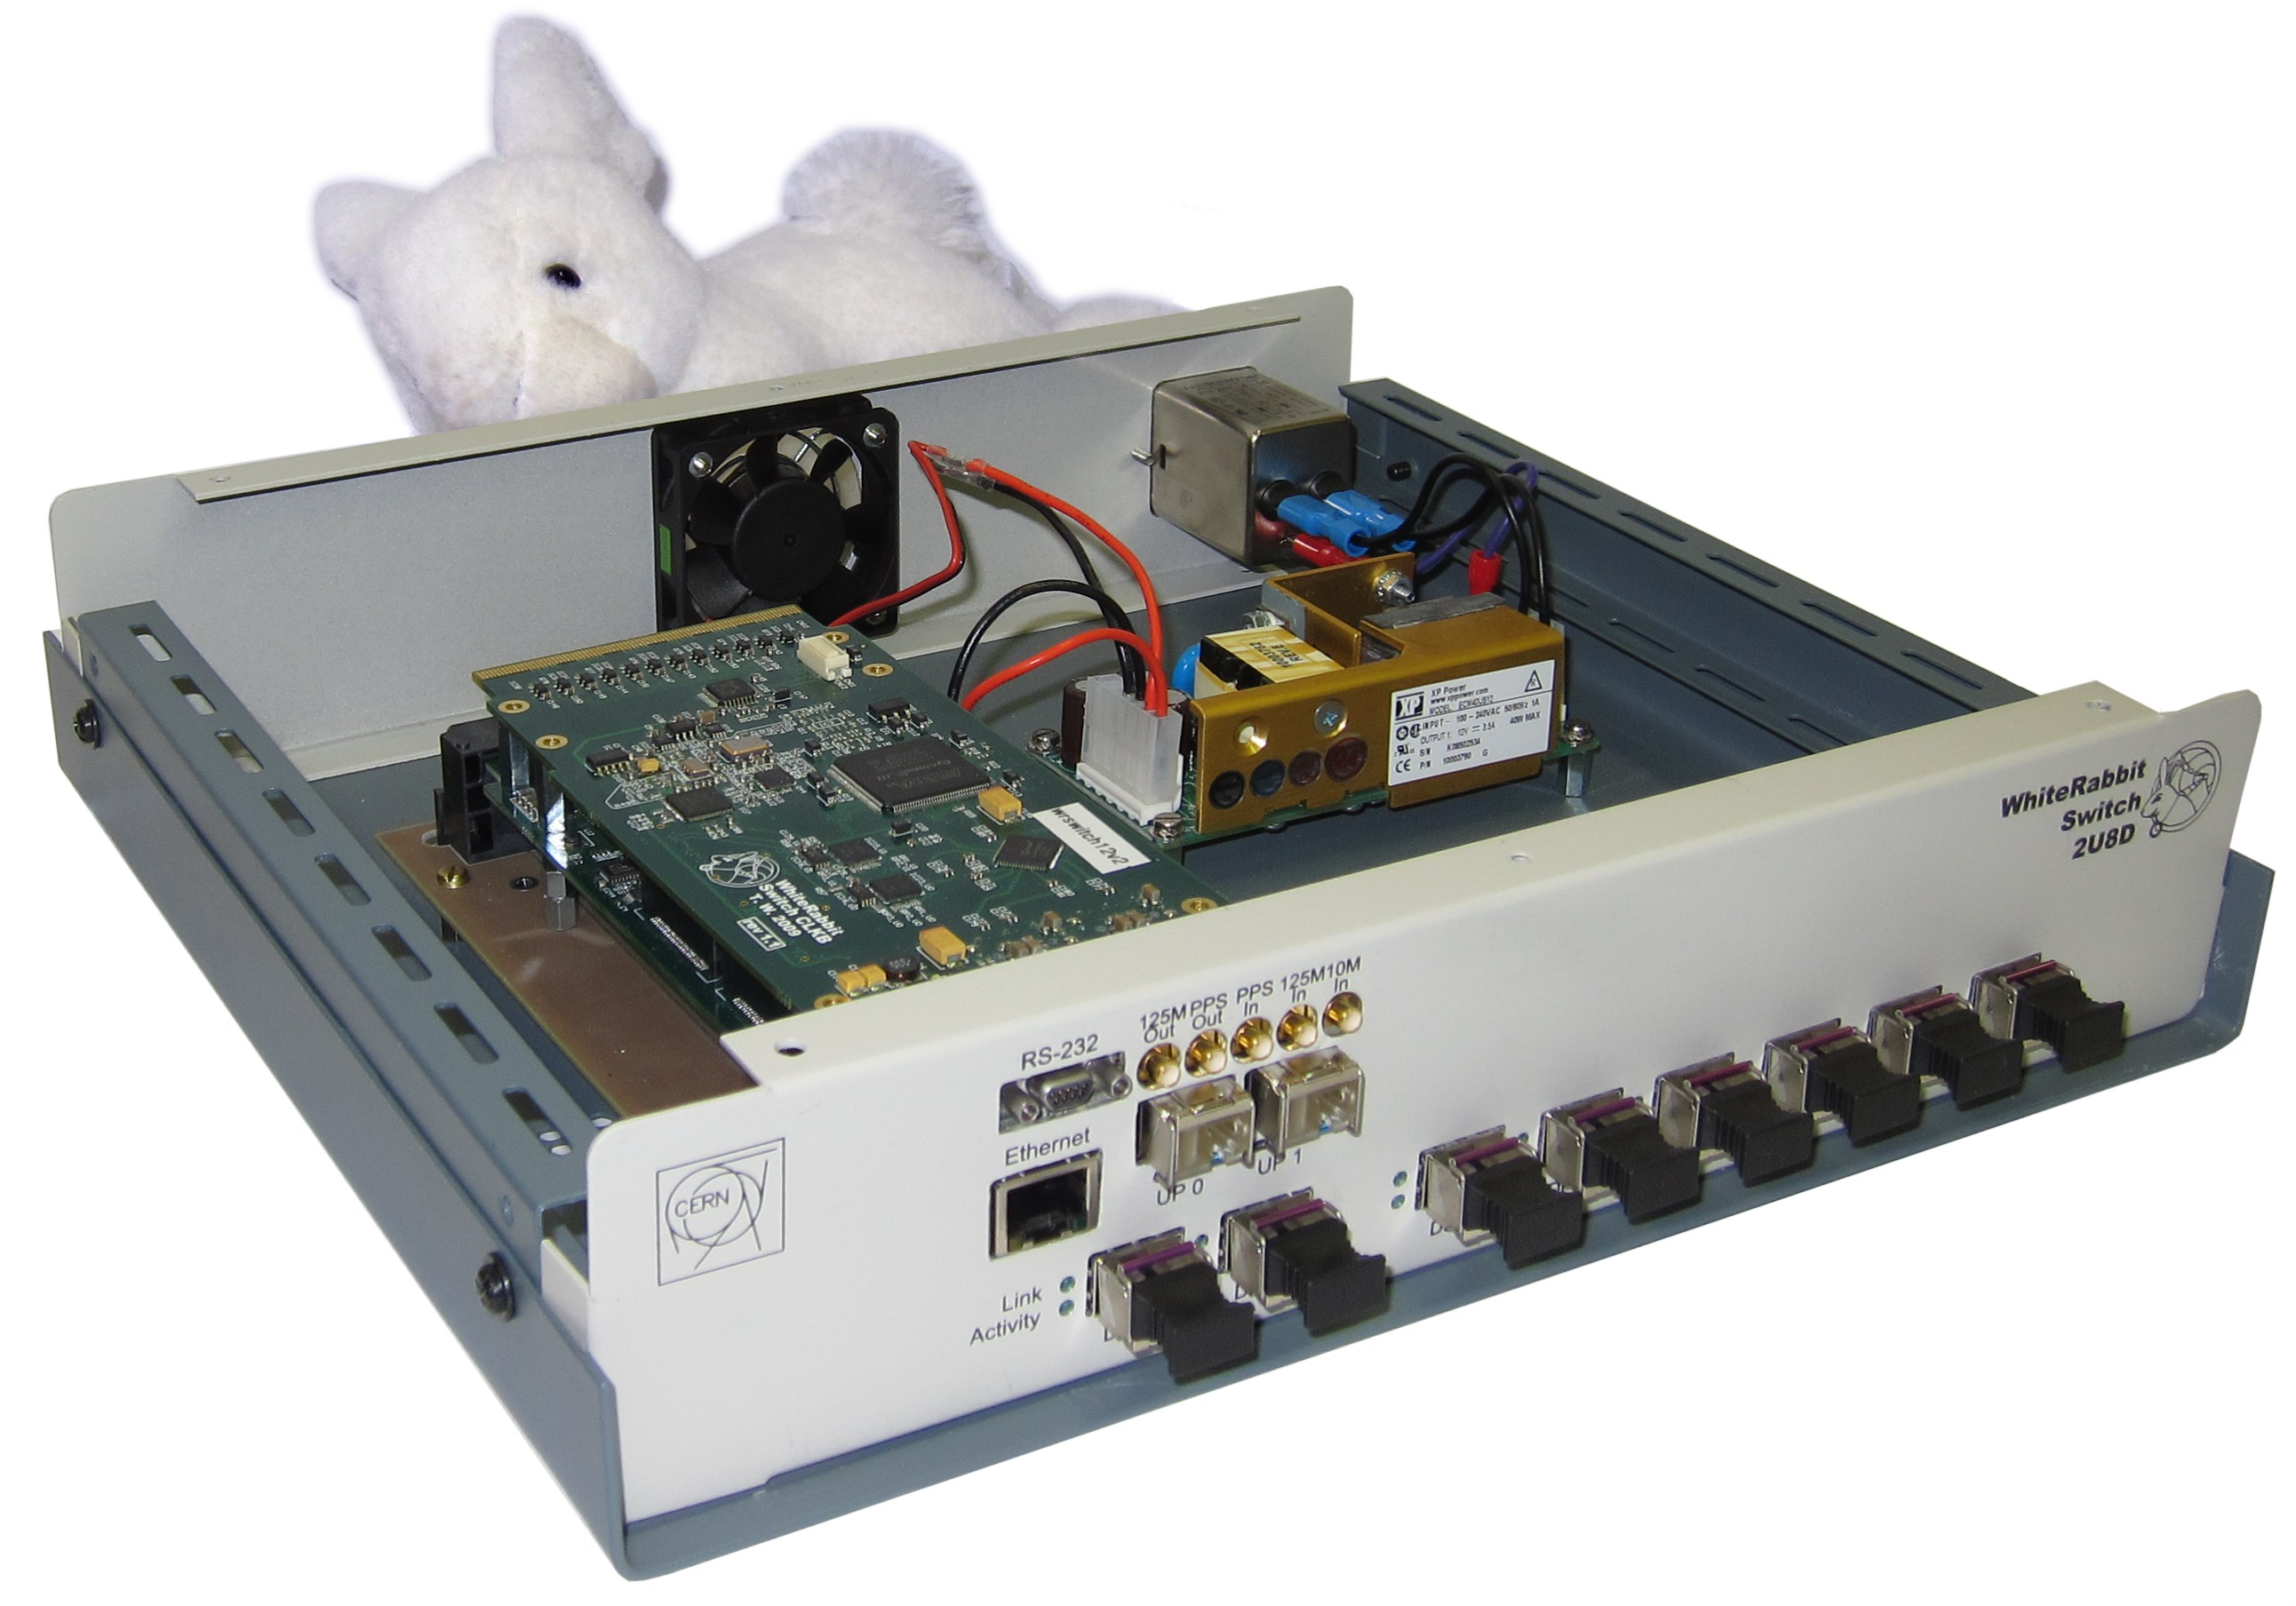
\includegraphics[width=7.0cm]{switch/wrs2_photo.jpg}
    \end{center}

	\begin{itemize}
	\item Centralny Element sieci White Rabbit
	\item Zbudowany od podstaw
	\item 10 portów 1000Base-LX 
	\item Embedded Linux
	\end{itemize}
\end{frame}
%%%%%%%%%%%%%%%%%%%%%%%%%%%%%%%%%%%%%%%%%%%%%%%%%%%%%%%%%%%%%%%%%%%%%%%%%%%%%%%%%%%%%%%%%%%%%%%%%%%%
% \subsection{}
%%%%%%%%%%%%%%%%%%%%%%%%%%%%%%%%%%%%%%%%%%%%%%%%%%%%%%%%%%%%%%%%%%%%%%%%%%%%%%%%%%%%%%%%%%%%%%%%%%%%
\begin{frame}{White Rabbit Switch (V2)}

    \begin{center}
    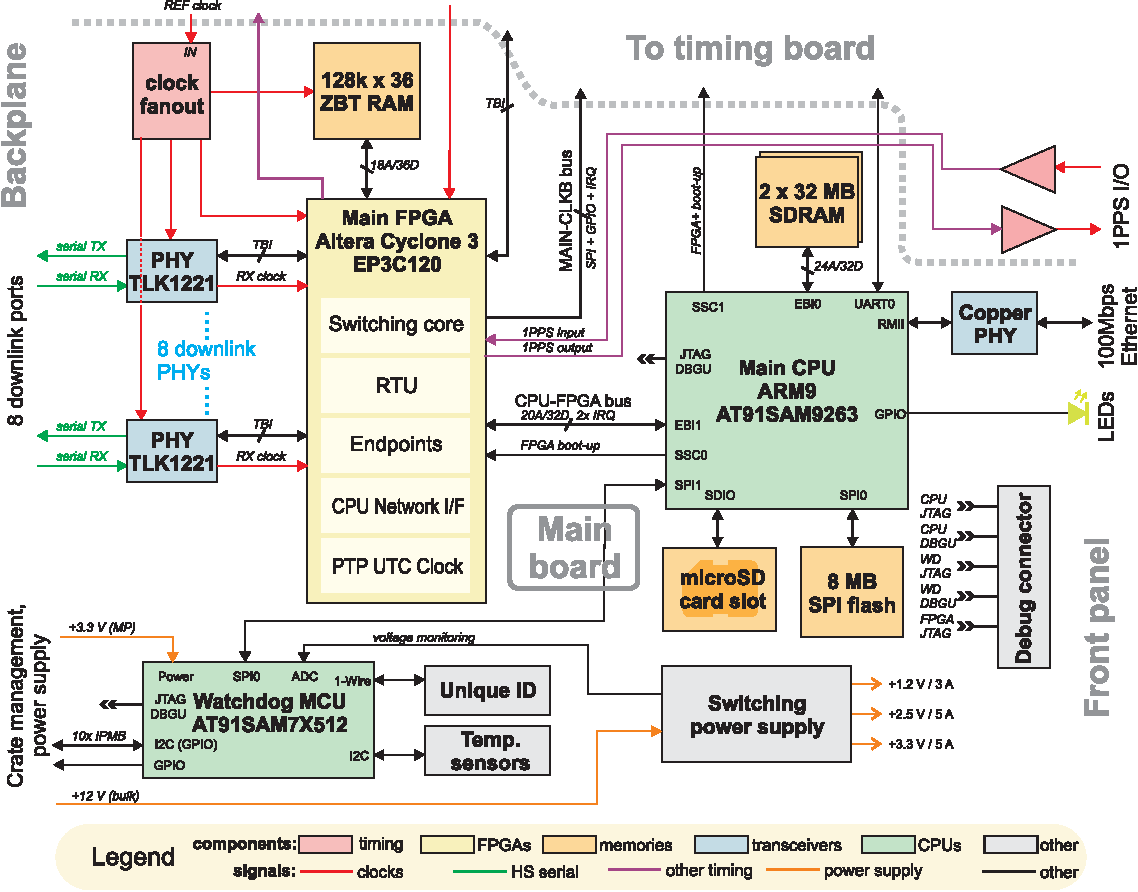
\includegraphics[width=7.0cm]{switch/wrs2_sw_block.pdf}
    \end{center}


\end{frame}
%%%%%%%%%%%%%%%%%%%%%%%%%%%%%%%%%%%%%%%%%%%%%%%%%%%%%%%%%%%%%%%%%%%%%%%%%%%%%%%%%%%%%%%%%%%%%%%%%%%%
% \subsection{}
%%%%%%%%%%%%%%%%%%%%%%%%%%%%%%%%%%%%%%%%%%%%%%%%%%%%%%%%%%%%%%%%%%%%%%%%%%%%%%%%%%%%%%%%%%%%%%%%%%%%
\begin{frame}{White Rabbit Node}

  \begin{columns}[c]
  \column{.4\textwidth} 

  \begin{itemize}
    \item WRPTP stack
    \item Koder/dekoder korekcji nadmiarowej
    \item Deterministyczny wbudowany mikroprocesor
    \item Etherbone - Wishbone po UDP
  \end{itemize}

      %\vspace{2cm}

  \column{.6\textwidth} 

    \begin{center}
    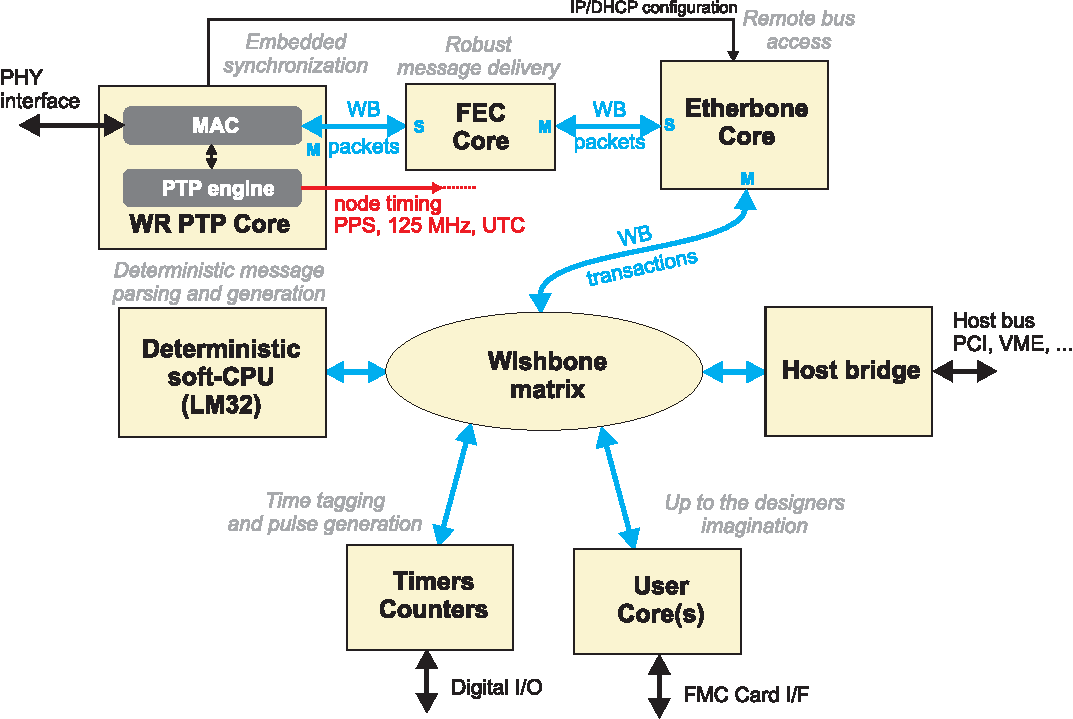
\includegraphics[width=7.0cm]{node/wr_node_block.pdf}
    \end{center}

%      \vspace{2cm}

  \end{columns}



\end{frame}
%%%%%%%%%%%%%%%%%%%%%%%%%%%%%%%%%%%%%%%%%%%%%%%%%%%%%%%%%%%%%%%%%%%%%%%%%%%%%%%%%%%%%%%%%%%%%%%%%%%%
% \subsection{}
%%%%%%%%%%%%%%%%%%%%%%%%%%%%%%%%%%%%%%%%%%%%%%%%%%%%%%%%%%%%%%%%%%%%%%%%%%%%%%%%%%%%%%%%%%%%%%%%%%%%
\begin{frame}{WR PTP Core}

%  \begin{columns}[c]
%  \column{.5\textwidth} 


%      \vspace{2cm}

%  \column{.5\textwidth} 

    \begin{center}
    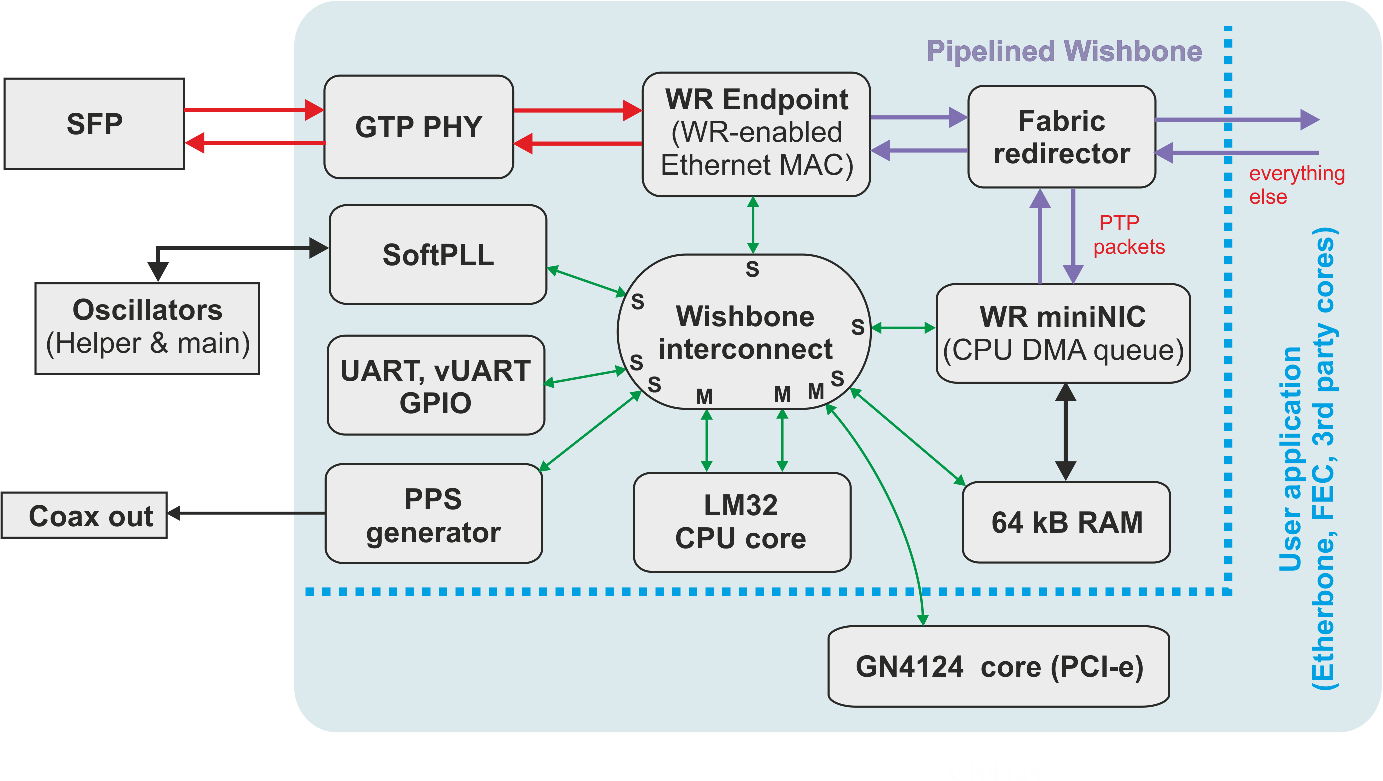
\includegraphics[width=8.0cm]{node/wrpc_v1.pdf}
    \end{center}

  \begin{itemize}
    \item Implementacja (HDL/SW) protokołu WRPTP w FPGA
    \item Deamon WRPTP działa na wbudowanym CPU
    \item Outputs: PPS, 125MHz, UTC
  \end{itemize}


%      \vspace{2cm}

  %\end{columns}



\end{frame}
%%%%%%%%%%%%%%%%%%%%%%%%%%%%%%%%%%%%%%%%%%%%%%%%%%%%%%%%%%%%%%%%%%%%%%%%%%%%%%%%%%%%%%%%%%%%%%%%%%%%
% \subsection{}
%%%%%%%%%%%%%%%%%%%%%%%%%%%%%%%%%%%%%%%%%%%%%%%%%%%%%%%%%%%%%%%%%%%%%%%%%%%%%%%%%%%%%%%%%%%%%%%%%%%%
\begin{frame}{Simple PCIe FMC carrier (SPEC)}

    \begin{center}
    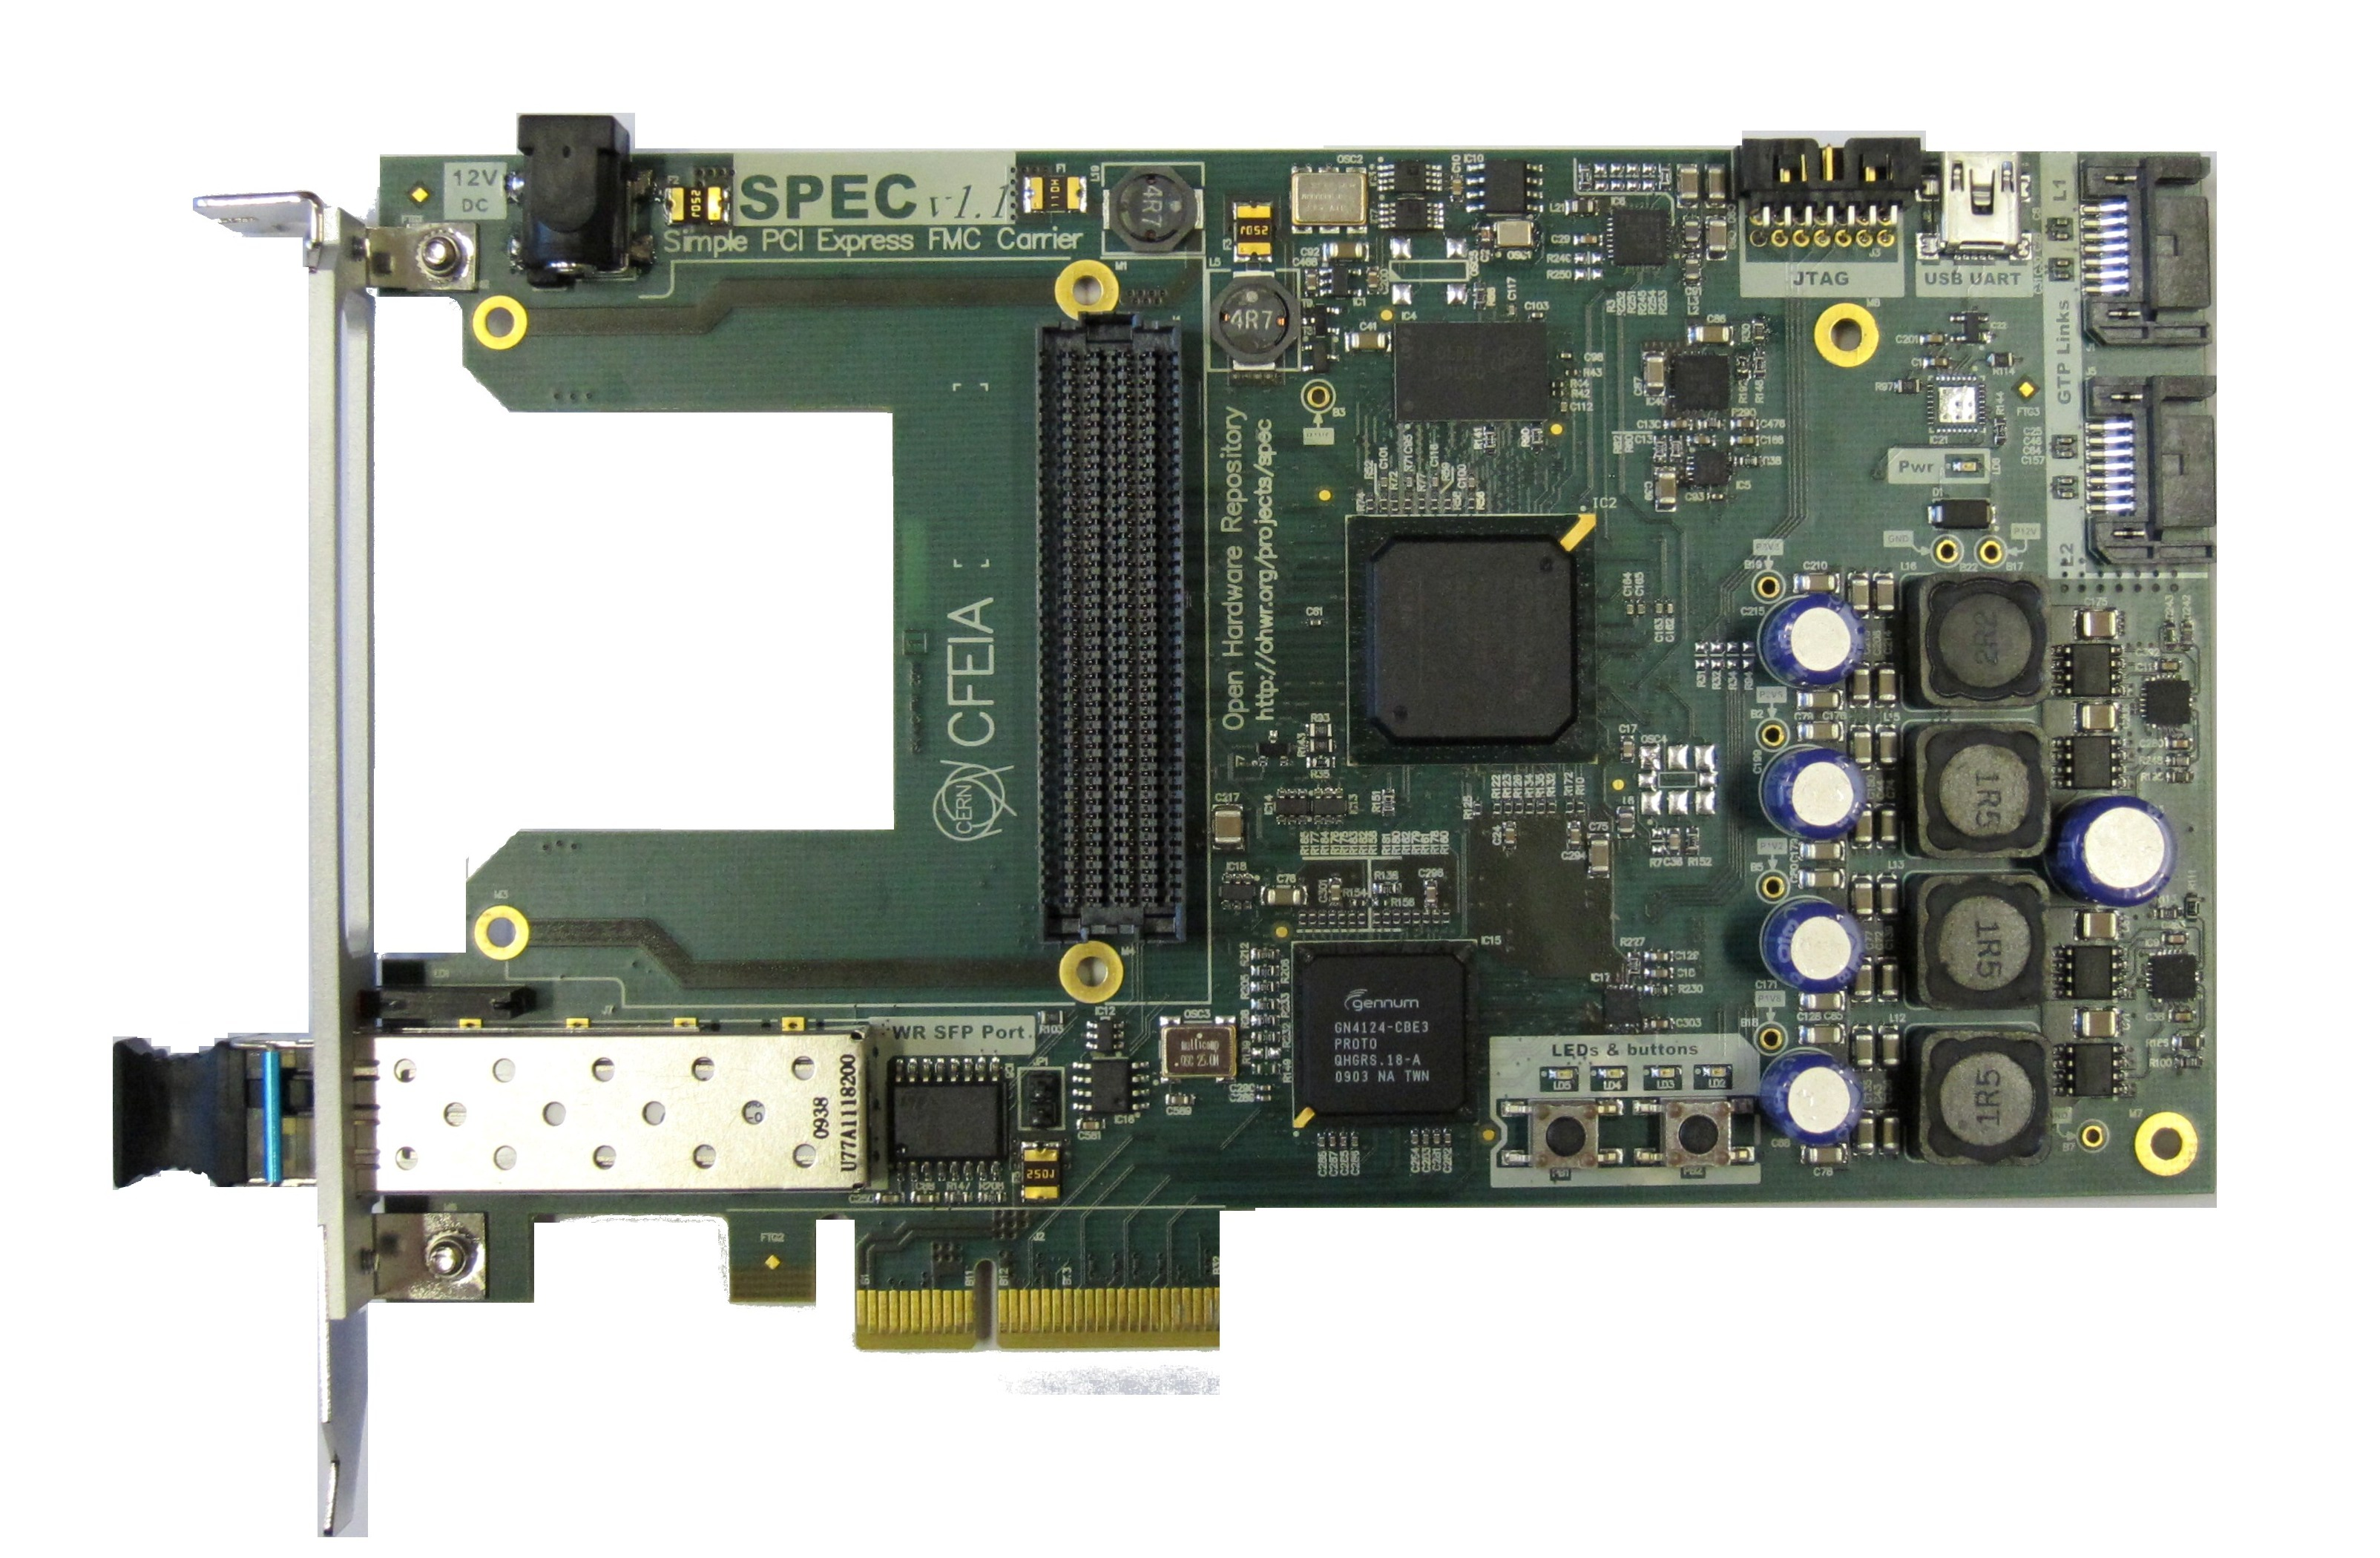
\includegraphics[width=8.0cm]{node/spec_photo.jpg}
    \end{center}


\end{frame}
%%%%%%%%%%%%%%%%%%%%%%%%%%%%%%%%%%%%%%%%%%%%%%%%%%%%%%%%%%%%%%%%%%%%%%%%%%%%%%%%%%%%%%%%%%%%%%%%%%%%
% \subsection{}
%%%%%%%%%%%%%%%%%%%%%%%%%%%%%%%%%%%%%%%%%%%%%%%%%%%%%%%%%%%%%%%%%%%%%%%%%%%%%%%%%%%%%%%%%%%%%%%%%%%%
\begin{frame}{WR-compliant Hardware Kit}

    \begin{center}
    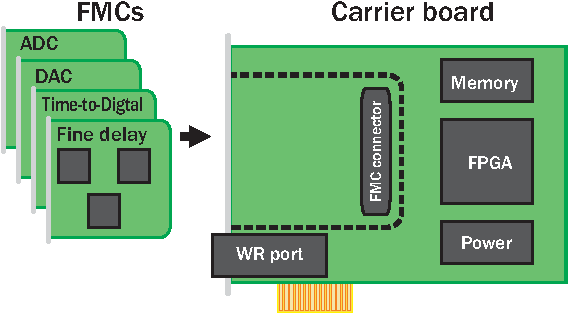
\includegraphics[width=6cm]{node/shw_kit}
    \end{center}

  \begin{columns}[c]
    \column{.01\textwidth}
    \column{.98\textwidth}

	\begin{block}{Co-HT FMC-based Hardware Kit:}
	  \begin{itemize}
	  \item FMCs (FPGA Mezzanine Cards) with ADCs, DACs, TDCs, fine delays, digital I/O
	  \item Carrier boards in PCI-Express, VME and uTCA formats
	  \item All carriers are equipped with a White Rabbit port
	  \end{itemize}
	\end{block}

    \column{.01\textwidth}
  \end{columns}


\end{frame}

%%%%%%%%%%%%%%%%%%%%%%%%%%%%%%%%%%%%%%%%%%%%%%%%%%%%%%%%%%%%%%%%%%%%%%%%%%%%%%%%%%%%%%%%%%%%%%%%%%%%
%\section{}
%\subsection{}
%%%%%%%%%%%%%%%%%%%%%%%%%%%%%%%%%%%%%%%%%%%%%%%%%%%%%%%%%%%%%%%%%%%%%%%%%%%%%%%%%%%%%%%%%%%%%%%%%%%%
\begin{frame}{Dziękuje}

    \begin{center}
    Pytania ?
    \end{center}

    
    \begin{center}
%    \includegraphics[height=4.0cm]{fig/white_rabbit_by_kyoht.ps}
    
\includegraphics[height=4.0cm]{logo/WRlogo.pdf}
    \end{center}

\end{frame}
%%%%%%%%%%%%%%%%%%%%%%%%%%%%%%%%%%%%%%%%%%%%%%%%%%%%%%%%%%%%%%%%%%%%%%%%%%%%%%%%%%%%%%%%%%%%%%%%%%%%
\end{document}
